\documentclass{article}
\usepackage[utf8]{inputenc}
\usepackage{amsmath,amssymb,amsfonts,amsthm,enumerate}
\usepackage{eucal}
\usepackage{xcolor}
\usepackage{lscape}
\usepackage{tikz}
\usepackage{environ}
\usepackage{caption}
\usepackage{subcaption}
\usepackage{algorithm}
\usepackage{algpseudocode}
\usetikzlibrary{positioning, backgrounds}

\begin{document}

The next example shows how to apply the density based method applies in higher dimension. The key point is that the quadratic form must be well chosen.

Let $G$ be an $m\times m$ graph, represented by a symmetric adjacency matrix $J$ consisting of only zeros and ones. We will define a data set of size $N$ in $\mathbb{R}^m$ by taking $N$ random simulations of the Ising model associated to $E$, defined as follows: for every discrete vector $\sigma \in \{1,-1\}^m$, define the Hamiltonian energy by
\begin{equation}
\label{eq:isingham}
    H(\sigma)=-\sum_{i,j}
J_{i,j} \sigma_i \sigma_j
\end{equation}
We then fix a temperature parameter
$\beta>0$ and seek to approximate the 
Boltzmann distribution
\begin{equation}
    \label{eq:boltzmann}
P_{\beta}(\sigma)=\frac{1}{Z_{\beta}}
e^{-\beta H(\sigma)},\quad
Z_\beta = e^{-\beta H(\sigma)}.
\end{equation}

The data set is then produced by running the single-flip Metropolis algorithm for a large enough number of steps per site (we chose about 40000) to obtain a data set 
\[\mathcal{D}_{J,\beta,N}=
\{\sigma^1,...,\sigma^N\}
\subset \mathbb{R}^m,\] 
by interpretting the
spin states $\sigma$ as real vectors in
$\mathbb{R}^m$.
We generated $\mathcal{D}_{J,\beta,N}$ for three different graphs $J$ shown in Figure \ref{fig:isinggraphs}: an interval consisting of 30 sites, a circle with 30 sites, and a graph with three flares of length 14 each coming from the center, for a total of 43 vertices. For every one we chose $\beta=3.0$, and $N=20000$. 

\begin{figure}
\centering
 \begin{subfigure}[b]{.3\textwidth}
\begin{tikzpicture}[scale=.25]
\draw[color=white] (-6.5,-6) rectangle (6.5,6);


\draw[color=black!100,thick] (-4.833333,0)--(-4.500000,0);
\draw[color=black!100,thick] (-4.500000,0)--(-4.166667,0);
\draw[color=black!100,thick] (-4.166667,0)--(-3.833333,0);
\draw[color=black!100,thick] (-3.833333,0)--(-3.500000,0);
\draw[color=black!100,thick] (-3.500000,0)--(-3.166667,0);
\draw[color=black!100,thick] (-3.166667,0)--(-2.833333,0);
\draw[color=black!100,thick] (-2.833333,0)--(-2.500000,0);
\draw[color=black!100,thick] (-2.500000,0)--(-2.166667,0);
\draw[color=black!100,thick] (-2.166667,0)--(-1.833333,0);
\draw[color=black!100,thick] (-1.833333,0)--(-1.500000,0);
\draw[color=black!100,thick] (-1.500000,0)--(-1.166667,0);
\draw[color=black!100,thick] (-1.166667,0)--(-0.833333,0);
\draw[color=black!100,thick] (-0.833333,0)--(-0.500000,0);
\draw[color=black!100,thick] (-0.500000,0)--(-0.166667,0);
\draw[color=black!100,thick] (-0.166667,0)--(0.166667,0);
\draw[color=black!100,thick] (0.166667,0)--(0.500000,0);
\draw[color=black!100,thick] (0.500000,0)--(0.833333,0.0);
\draw[color=black!100,thick] (0.833333,0)--(1.166667,0);
\draw[color=black!100,thick] (1.166667,0)--(1.500000,0);
\draw[color=black!100,thick] (1.500000,0)--(1.833333,0);
\draw[color=black!100,thick] (1.833333,0)--(2.166667,0);
\draw[color=black!100,thick] (2.166667,0)--(2.500000,0);
\draw[color=black!100,thick] (2.500000,0)--(2.833333,0);
\draw[color=black!100,thick] (2.833333,0)--(3.166667,0);
\draw[color=black!100,thick] (3.166667,0)--(3.500000,0);
\draw[color=black!100,thick] (3.500000,0)--(3.833333,0);
\draw[color=black!100,thick] (3.833333,0)--(4.166667,0);
\draw[color=black!100,thick] (4.166667,0)--(4.500000,0);
\draw[color=black!100,thick] (4.5,0)--(5.166666,0);


\draw[color=black!100,fill=black!100,thick] (-4.833333,0) circle (4.0pt);

\draw[color=black!100,fill=black!100,thick] (-3.833333,0) circle (4.0pt);

\draw[color=black!100,fill=black!100,thick] (-2.833333,0) circle (4.0pt);

\draw[color=black!100,fill=black!100,thick] (-1.833333,0) circle (4.0pt);

\draw[color=black!100,fill=black!100,thick] (-0.833333,0) circle (4.0pt);

\draw[color=black!100,fill=black!100,thick] (0.166667,0) circle (4.0pt);

\draw[color=black!100,fill=black!100,thick] (1.166667,0) circle (4.0pt);

\draw[color=black!100,fill=black!100,thick] (2.166667,0) circle (4.0pt);

\draw[color=black!100,fill=black!100,thick] (3.166667,0) circle (4.0pt);

\draw[color=black!100,fill=black!100,thick] (4.166667,0) circle (4.0pt);

\draw[color=black!100,fill=black!100,thick] (5.1666667,0) circle (4.0pt);


\end{tikzpicture}
\end{subfigure}
\begin{subfigure}[b]{.3\textwidth}
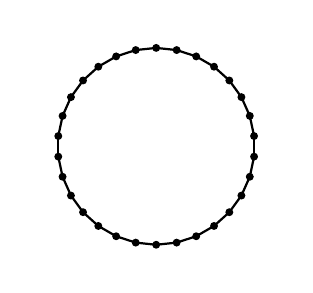
\begin{tikzpicture}[scale=.25]
\draw[color=white] (-6.5,-6) rectangle (6.5,6);


\draw[color=black!100,thick] (4.972609,0.522642)--(4.755283,1.545085);
\draw[color=black!100,thick] (4.755283,1.545085)--(4.330127,2.500000);
\draw[color=black!100,thick] (4.330127,2.500000)--(3.715724,3.345653);
\draw[color=black!100,thick] (3.715724,3.345653)--(2.938926,4.045085);
\draw[color=black!100,thick] (2.938926,4.045085)--(2.033683,4.567727);
\draw[color=black!100,thick] (2.033683,4.567727)--(1.039558,4.890738);
\draw[color=black!100,thick] (1.039558,4.890738)--(-0.000000,5.000000);
\draw[color=black!100,thick] (-0.000000,5.000000)--(-1.039558,4.890738);
\draw[color=black!100,thick] (-1.039558,4.890738)--(-2.033683,4.567727);
\draw[color=black!100,thick] (-2.033683,4.567727)--(-2.938926,4.045085);
\draw[color=black!100,thick] (-2.938926,4.045085)--(-3.715724,3.345653);
\draw[color=black!100,thick] (-3.715724,3.345653)--(-4.330127,2.500000);
\draw[color=black!100,thick] (-4.330127,2.500000)--(-4.755283,1.545085);
\draw[color=black!100,thick] (-4.755283,1.545085)--(-4.972609,0.522642);
\draw[color=black!100,thick] (-4.972609,0.522642)--(-4.972609,-0.522642);
\draw[color=black!100,thick] (-4.972609,-0.522642)--(-4.755283,-1.545085);
\draw[color=black!100,thick] (-4.755283,-1.545085)--(-4.330127,-2.500000);
\draw[color=black!100,thick] (-4.330127,-2.500000)--(-3.715724,-3.345653);
\draw[color=black!100,thick] (-3.715724,-3.345653)--(-2.938926,-4.045085);
\draw[color=black!100,thick] (-2.938926,-4.045085)--(-2.033683,-4.567727);
\draw[color=black!100,thick] (-2.033683,-4.567727)--(-1.039558,-4.890738);
\draw[color=black!100,thick] (-1.039558,-4.890738)--(0.000000,-5.000000);
\draw[color=black!100,thick] (0.000000,-5.000000)--(1.039558,-4.890738);
\draw[color=black!100,thick] (1.039558,-4.890738)--(2.033683,-4.567727);
\draw[color=black!100,thick] (2.033683,-4.567727)--(2.938926,-4.045085);
\draw[color=black!100,thick] (2.938926,-4.045085)--(3.715724,-3.345653);
\draw[color=black!100,thick] (3.715724,-3.345653)--(4.330127,-2.500000);
\draw[color=black!100,thick] (4.330127,-2.500000)--(4.755283,-1.545085);
\draw[color=black!100,thick] (4.755283,-1.545085)--(4.972609,-0.522642);
\draw[color=black!100,thick] (4.972609,-0.522642)--(4.972609,0.522642);


\draw[color=black!100,fill=black!100,thick] (4.972609,0.522642) circle (4.0pt);
\draw[color=black!100,fill=black!100,thick] (4.755283,1.545085) circle (4.0pt);
\draw[color=black!100,fill=black!100,thick] (4.330127,2.500000) circle (4.0pt);
\draw[color=black!100,fill=black!100,thick] (3.715724,3.345653) circle (4.0pt);
\draw[color=black!100,fill=black!100,thick] (2.938926,4.045085) circle (4.0pt);
\draw[color=black!100,fill=black!100,thick] (2.033683,4.567727) circle (4.0pt);
\draw[color=black!100,fill=black!100,thick] (1.039558,4.890738) circle (4.0pt);
\draw[color=black!100,fill=black!100,thick] (-0.000000,5.000000) circle (4.0pt);
\draw[color=black!100,fill=black!100,thick] (-1.039558,4.890738) circle (4.0pt);
\draw[color=black!100,fill=black!100,thick] (-2.033683,4.567727) circle (4.0pt);
\draw[color=black!100,fill=black!100,thick] (-2.938926,4.045085) circle (4.0pt);
\draw[color=black!100,fill=black!100,thick] (-3.715724,3.345653) circle (4.0pt);
\draw[color=black!100,fill=black!100,thick] (-4.330127,2.500000) circle (4.0pt);
\draw[color=black!100,fill=black!100,thick] (-4.755283,1.545085) circle (4.0pt);
\draw[color=black!100,fill=black!100,thick] (-4.972609,0.522642) circle (4.0pt);
\draw[color=black!100,fill=black!100,thick] (-4.972609,-0.522642) circle (4.0pt);
\draw[color=black!100,fill=black!100,thick] (-4.755283,-1.545085) circle (4.0pt);
\draw[color=black!100,fill=black!100,thick] (-4.330127,-2.500000) circle (4.0pt);
\draw[color=black!100,fill=black!100,thick] (-3.715724,-3.345653) circle (4.0pt);
\draw[color=black!100,fill=black!100,thick] (-2.938926,-4.045085) circle (4.0pt);
\draw[color=black!100,fill=black!100,thick] (-2.033683,-4.567727) circle (4.0pt);
\draw[color=black!100,fill=black!100,thick] (-1.039558,-4.890738) circle (4.0pt);
\draw[color=black!100,fill=black!100,thick] (0.000000,-5.000000) circle (4.0pt);
\draw[color=black!100,fill=black!100,thick] (1.039558,-4.890738) circle (4.0pt);
\draw[color=black!100,fill=black!100,thick] (2.033683,-4.567727) circle (4.0pt);
\draw[color=black!100,fill=black!100,thick] (2.938926,-4.045085) circle (4.0pt);
\draw[color=black!100,fill=black!100,thick] (3.715724,-3.345653) circle (4.0pt);
\draw[color=black!100,fill=black!100,thick] (4.330127,-2.500000) circle (4.0pt);
\draw[color=black!100,fill=black!100,thick] (4.755283,-1.545085) circle (4.0pt);
\draw[color=black!100,fill=black!100,thick] (4.972609,-0.522642) circle (4.0pt);
\end{tikzpicture}
\end{subfigure}
\begin{subfigure}[b]{.3\textwidth}
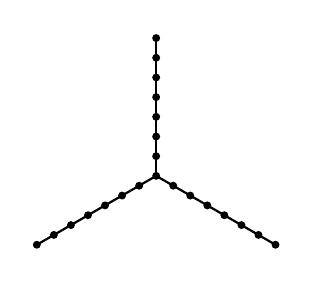
\begin{tikzpicture}[scale=.25]
\draw[color=white] (-6.5,-4.5) rectangle (6.5,7.5);

\draw[color=black!100,thick] (0.000000,0.000000)--(0.000000,0.500000);
\draw[color=black!100,thick] (0.000000,0.500000)--(0.000000,1.000000);
\draw[color=black!100,thick] (0.000000,1.000000)--(0.000000,1.500000);
\draw[color=black!100,thick] (0.000000,1.500000)--(0.000000,2.000000);
\draw[color=black!100,thick] (0.000000,2.000000)--(0.000000,2.500000);
\draw[color=black!100,thick] (0.000000,2.500000)--(0.000000,3.000000);
\draw[color=black!100,thick] (0.000000,3.000000)--(0.000000,3.500000);
\draw[color=black!100,thick] (0.000000,3.500000)--(0.000000,4.000000);
\draw[color=black!100,thick] (0.000000,4.000000)--(0.000000,4.500000);
\draw[color=black!100,thick] (0.000000,4.500000)--(0.000000,5.000000);
\draw[color=black!100,thick] (0.000000,5.000000)--(0.000000,5.500000);
\draw[color=black!100,thick] (0.000000,5.500000)--(0.000000,6.000000);
\draw[color=black!100,thick] (0.000000,6.000000)--(0.000000,6.500000);
\draw[color=black!100,thick] (0.000000,6.500000)--(0.000000,7.000000);

\draw[color=black!100,thick] (0.000000,0.000000)--(-0.433013,-0.250000);
\draw[color=black!100,thick] (-0.433013,-0.250000)--(-0.866025,-0.500000);
\draw[color=black!100,thick] (-0.866025,-0.500000)--(-1.299038,-0.750000);
\draw[color=black!100,thick] (-1.299038,-0.750000)--(-1.732051,-1.000000);
\draw[color=black!100,thick] (-1.732051,-1.000000)--(-2.165064,-1.250000);
\draw[color=black!100,thick] (-2.165064,-1.250000)--(-2.598076,-1.500000);
\draw[color=black!100,thick] (-2.598076,-1.500000)--(-3.031089,-1.750000);
\draw[color=black!100,thick] (-3.031089,-1.750000)--(-3.464102,-2.000000);
\draw[color=black!100,thick] (-3.464102,-2.000000)--(-3.897114,-2.250000);
\draw[color=black!100,thick] (-3.897114,-2.250000)--(-4.330127,-2.500000);
\draw[color=black!100,thick] (-4.330127,-2.500000)--(-4.763140,-2.750000);
\draw[color=black!100,thick] (-4.763140,-2.750000)--(-5.196152,-3.000000);
\draw[color=black!100,thick] (-5.196152,-3.000000)--(-5.629165,-3.250000);
\draw[color=black!100,thick] (-5.629165,-3.250000)--(-6.062178,-3.500000);


\draw[color=black!100,thick] (0.000000,0.000000)--(0.433013,-0.250000);
\draw[color=black!100,thick] (0.433013,-0.250000)--(0.866025,-0.500000);
\draw[color=black!100,thick] (0.866025,-0.500000)--(1.299038,-0.750000);
\draw[color=black!100,thick] (1.299038,-0.750000)--(1.732051,-1.000000);
\draw[color=black!100,thick] (1.732051,-1.000000)--(2.165064,-1.250000);
\draw[color=black!100,thick] (2.165064,-1.250000)--(2.598076,-1.500000);
\draw[color=black!100,thick] (2.598076,-1.500000)--(3.031089,-1.750000);
\draw[color=black!100,thick] (3.031089,-1.750000)--(3.464102,-2.000000);
\draw[color=black!100,thick] (3.464102,-2.000000)--(3.897114,-2.250000);
\draw[color=black!100,thick] (3.897114,-2.250000)--(4.330127,-2.500000);
\draw[color=black!100,thick] (4.330127,-2.500000)--(4.763140,-2.750000);
\draw[color=black!100,thick] (4.763140,-2.750000)--(5.196152,-3.000000);
\draw[color=black!100,thick] (5.196152,-3.000000)--(5.629165,-3.250000);
\draw[color=black!100,thick] (5.629165,-3.250000)--(6.062178,-3.500000);


\draw[color=black!100,fill=black!100,thick] (0.000000,1.000000) circle (4.0pt);
\draw[color=black!100,fill=black!100,thick] (0.000000,2.000000) circle (4.0pt);
\draw[color=black!100,fill=black!100,thick] (0.000000,3.000000) circle (4.0pt);
\draw[color=black!100,fill=black!100,thick] (0.000000,4.000000) circle (4.0pt);
\draw[color=black!100,fill=black!100,thick] (0.000000,5.000000) circle (4.0pt);
\draw[color=black!100,fill=black!100,thick] (0.000000,6.000000) circle (4.0pt);
\draw[color=black!100,fill=black!100,thick] (0.000000,7.000000) circle (4.0pt);


\draw[color=black!100,fill=black!100,thick] (0.866025,-0.500000) circle (4.0pt);
\draw[color=black!100,fill=black!100,thick] (1.732051,-1.000000) circle (4.0pt);
\draw[color=black!100,fill=black!100,thick] (2.598076,-1.500000) circle (4.0pt);
\draw[color=black!100,fill=black!100,thick] (3.464102,-2.000000) circle (4.0pt);
\draw[color=black!100,fill=black!100,thick] (4.330127,-2.500000) circle (4.0pt);
\draw[color=black!100,fill=black!100,thick] (5.196152,-3.000000) circle (4.0pt);
\draw[color=black!100,fill=black!100,thick] (6.062178,-3.500000) circle (4.0pt);


\draw[color=black!100,fill=black!100,thick] (-0.866025,-0.500000) circle (4.0pt);
\draw[color=black!100,fill=black!100,thick] (-1.732051,-1.000000) circle (4.0pt);
\draw[color=black!100,fill=black!100,thick] (-2.598076,-1.500000) circle (4.0pt);
\draw[color=black!100,fill=black!100,thick] (-3.464102,-2.000000) circle (4.0pt);
\draw[color=black!100,fill=black!100,thick] (-4.330127,-2.500000) circle (4.0pt);
\draw[color=black!100,fill=black!100,thick] (-5.196152,-3.000000) circle (4.0pt);
\draw[color=black!100,fill=black!100,thick] (-6.062178,-3.500000) circle (4.0pt);

\draw[color=black!100,fill=black!100,thick] (0.000000,0.000000) circle (4.0pt);

\end{tikzpicture}
\end{subfigure}

 \centering
 
\begin{subfigure}[b]{.4\textwidth}
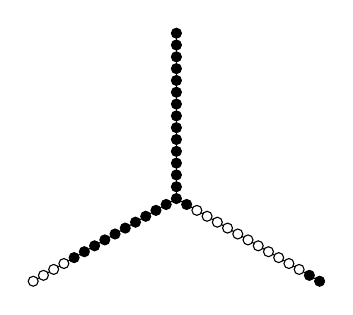
\begin{tikzpicture}[scale=.3]

\draw[color=black!100,thin] (0.000000,0.000000)--(0.000000,0.500000);
\draw[color=black!100,thin] (0.000000,0.500000)--(0.000000,1.000000);
\draw[color=black!100,thin] (0.000000,1.000000)--(0.000000,1.500000);
\draw[color=black!100,thin] (0.000000,1.500000)--(0.000000,2.000000);
\draw[color=black!100,thin] (0.000000,2.000000)--(0.000000,2.500000);
\draw[color=black!100,thin] (0.000000,2.500000)--(0.000000,3.000000);
\draw[color=black!100,thin] (0.000000,3.000000)--(0.000000,3.500000);
\draw[color=black!100,thin] (0.000000,3.500000)--(0.000000,4.000000);
\draw[color=black!100,thin] (0.000000,4.000000)--(0.000000,4.500000);
\draw[color=black!100,thin] (0.000000,4.500000)--(0.000000,5.000000);
\draw[color=black!100,thin] (0.000000,5.000000)--(0.000000,5.500000);
\draw[color=black!100,thin] (0.000000,5.500000)--(0.000000,6.000000);
\draw[color=black!100,thin] (0.000000,6.000000)--(0.000000,6.500000);
\draw[color=black!100,thin] (0.000000,6.500000)--(0.000000,7.000000);

\draw[color=black!100,thin] (0.000000,0.000000)--(-0.433013,-0.250000);
\draw[color=black!100,thin] (-0.433013,-0.250000)--(-0.866025,-0.500000);
\draw[color=black!100,thin] (-0.866025,-0.500000)--(-1.299038,-0.750000);
\draw[color=black!100,thin] (-1.299038,-0.750000)--(-1.732051,-1.000000);
\draw[color=black!100,thin] (-1.732051,-1.000000)--(-2.165064,-1.250000);
\draw[color=black!100,thin] (-2.165064,-1.250000)--(-2.598076,-1.500000);
\draw[color=black!100,thin] (-2.598076,-1.500000)--(-3.031089,-1.750000);
\draw[color=black!100,thin] (-3.031089,-1.750000)--(-3.464102,-2.000000);
\draw[color=black!100,thin] (-3.464102,-2.000000)--(-3.897114,-2.250000);
\draw[color=black!100,thin] (-3.897114,-2.250000)--(-4.330127,-2.500000);
\draw[color=black!100,thin] (-4.330127,-2.500000)--(-4.763140,-2.750000);
\draw[color=black!100,thin] (-4.763140,-2.750000)--(-5.196152,-3.000000);
\draw[color=black!100,thin] (-5.196152,-3.000000)--(-5.629165,-3.250000);
\draw[color=black!100,thin] (-5.629165,-3.250000)--(-6.062178,-3.500000);


\draw[color=black!100,thin] (0.000000,0.000000)--(0.433013,-0.250000);
\draw[color=black!100,thin] (0.433013,-0.250000)--(0.866025,-0.500000);
\draw[color=black!100,thin] (0.866025,-0.500000)--(1.299038,-0.750000);
\draw[color=black!100,thin] (1.299038,-0.750000)--(1.732051,-1.000000);
\draw[color=black!100,thin] (1.732051,-1.000000)--(2.165064,-1.250000);
\draw[color=black!100,thin] (2.165064,-1.250000)--(2.598076,-1.500000);
\draw[color=black!100,thin] (2.598076,-1.500000)--(3.031089,-1.750000);
\draw[color=black!100,thin] (3.031089,-1.750000)--(3.464102,-2.000000);
\draw[color=black!100,thin] (3.464102,-2.000000)--(3.897114,-2.250000);
\draw[color=black!100,thin] (3.897114,-2.250000)--(4.330127,-2.500000);
\draw[color=black!100,thin] (4.330127,-2.500000)--(4.763140,-2.750000);
\draw[color=black!100,thin] (4.763140,-2.750000)--(5.196152,-3.000000);
\draw[color=black!100,thin] (5.196152,-3.000000)--(5.629165,-3.250000);
\draw[color=black!100,thin] (5.629165,-3.250000)--(6.062178,-3.500000);


\draw[color=black!100,fill=black!100,thin] (0.000000,0.500000) circle (6.0pt);
\draw[color=black!100,fill=black!100,thin] (0.000000,1.000000) circle (6.0pt);
\draw[color=black!100,fill=black!100,thin] (0.000000,1.500000) circle (6.0pt);
\draw[color=black!100,fill=black!100,thin] (0.000000,2.000000) circle (6.0pt);
\draw[color=black!100,fill=black!100,thin] (0.000000,2.500000) circle (6.0pt);
\draw[color=black!100,fill=black!100,thin] (0.000000,3.000000) circle (6.0pt);
\draw[color=black!100,fill=black!100,thin] (0.000000,3.500000) circle (6.0pt);
\draw[color=black!100,fill=black!100,thin] (0.000000,4.000000) circle (6.0pt);
\draw[color=black!100,fill=black!100,thin] (0.000000,4.500000) circle (6.0pt);
\draw[color=black!100,fill=black!100,thin] (0.000000,5.000000) circle (6.0pt);
\draw[color=black!100,fill=black!100,thin] (0.000000,5.500000) circle (6.0pt);
\draw[color=black!100,fill=black!100,thin] (0.000000,6.000000) circle (6.0pt);
\draw[color=black!100,fill=black!100,thin] (0.000000,6.500000) circle (6.0pt);
\draw[color=black!100,fill=black!100,thin] (0.000000,7.000000) circle (6.0pt);



\draw[color=black!100,fill=black!100,thin] (0.433013,-0.250000) circle (6.0pt);
\draw[color=black!100,fill=black!0,thin] (0.866025,-0.500000) circle (6.0pt);
\draw[color=black!100,fill=black!0,thin] (1.299038,-0.750000) circle (6.0pt);
\draw[color=black!100,fill=black!0,thin] (1.732051,-1.000000) circle (6.0pt);
\draw[color=black!100,fill=black!0,thin] (2.165064,-1.250000) circle (6.0pt);
\draw[color=black!100,fill=black!0,thin] (2.598076,-1.500000) circle (6.0pt);
\draw[color=black!100,fill=black!0,thin] (3.031089,-1.750000) circle (6.0pt);
\draw[color=black!100,fill=black!0,thin] (3.464102,-2.000000) circle (6.0pt);
\draw[color=black!100,fill=black!0,thin] (3.897114,-2.250000) circle (6.0pt);
\draw[color=black!100,fill=black!0,thin] (4.330127,-2.500000) circle (6.0pt);
\draw[color=black!100,fill=black!0,thin] (4.763140,-2.750000) circle (6.0pt);
\draw[color=black!100,fill=black!0,thin] (5.196152,-3.000000) circle (6.0pt);
\draw[color=black!100,fill=black!100,thin] (5.629165,-3.250000) circle (6.0pt);
\draw[color=black!100,fill=black!100,thin] (6.062178,-3.500000) circle (6.0pt);




\draw[color=black!100,fill=black!100,thin] (-0.433013,-0.250000) circle (6.0pt);
\draw[color=black!100,fill=black!100,thin] (-0.866025,-0.500000) circle (6.0pt);
\draw[color=black!100,fill=black!100,thin] (-1.299038,-0.750000) circle (6.0pt);
\draw[color=black!100,fill=black!100,thin] (-1.732051,-1.000000) circle (6.0pt);
\draw[color=black!100,fill=black!100,thin] (-2.165064,-1.250000) circle (6.0pt);
\draw[color=black!100,fill=black!100,thin] (-2.598076,-1.500000) circle (6.0pt);
\draw[color=black!100,fill=black!100,thin] (-3.031089,-1.750000) circle (6.0pt);
\draw[color=black!100,fill=black!100,thin] (-3.464102,-2.000000) circle (6.0pt);
\draw[color=black!100,fill=black!100,thin] (-3.897114,-2.250000) circle (6.0pt);
\draw[color=black!100,fill=black!100,thin] (-4.330127,-2.500000) circle (6.0pt);
\draw[color=black!100,fill=black!0,thin] (-4.763140,-2.750000) circle (6.0pt);
\draw[color=black!100,fill=black!0,thin] (-5.196152,-3.000000) circle (6.0pt);
\draw[color=black!100,fill=black!0,thin] (-5.629165,-3.250000) circle (6.0pt);
\draw[color=black!100,fill=black!0,thin] (-6.062178,-3.500000) circle (6.0pt);


\draw[color=black!100,fill=black!100,thin] (0.000000,0.000000) circle (6.0pt);


\end{tikzpicture}
\end{subfigure}
\begin{subfigure}[b]{.4\textwidth}
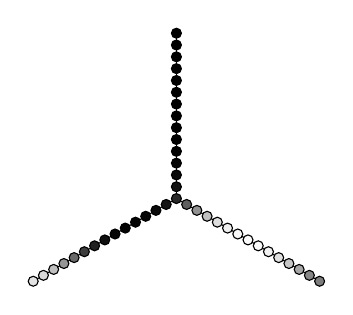
\begin{tikzpicture}[scale=.3]

\draw[color=black!100,thin] (0.000000,0.000000)--(0.000000,0.500000);
\draw[color=black!100,thin] (0.000000,0.500000)--(0.000000,1.000000);
\draw[color=black!100,thin] (0.000000,1.000000)--(0.000000,1.500000);
\draw[color=black!100,thin] (0.000000,1.500000)--(0.000000,2.000000);
\draw[color=black!100,thin] (0.000000,2.000000)--(0.000000,2.500000);
\draw[color=black!100,thin] (0.000000,2.500000)--(0.000000,3.000000);
\draw[color=black!100,thin] (0.000000,3.000000)--(0.000000,3.500000);
\draw[color=black!100,thin] (0.000000,3.500000)--(0.000000,4.000000);
\draw[color=black!100,thin] (0.000000,4.000000)--(0.000000,4.500000);
\draw[color=black!100,thin] (0.000000,4.500000)--(0.000000,5.000000);
\draw[color=black!100,thin] (0.000000,5.000000)--(0.000000,5.500000);
\draw[color=black!100,thin] (0.000000,5.500000)--(0.000000,6.000000);
\draw[color=black!100,thin] (0.000000,6.000000)--(0.000000,6.500000);
\draw[color=black!100,thin] (0.000000,6.500000)--(0.000000,7.000000);

\draw[color=black!100,thin] (0.000000,0.000000)--(-0.433013,-0.250000);
\draw[color=black!100,thin] (-0.433013,-0.250000)--(-0.866025,-0.500000);
\draw[color=black!100,thin] (-0.866025,-0.500000)--(-1.299038,-0.750000);
\draw[color=black!100,thin] (-1.299038,-0.750000)--(-1.732051,-1.000000);
\draw[color=black!100,thin] (-1.732051,-1.000000)--(-2.165064,-1.250000);
\draw[color=black!100,thin] (-2.165064,-1.250000)--(-2.598076,-1.500000);
\draw[color=black!100,thin] (-2.598076,-1.500000)--(-3.031089,-1.750000);
\draw[color=black!100,thin] (-3.031089,-1.750000)--(-3.464102,-2.000000);
\draw[color=black!100,thin] (-3.464102,-2.000000)--(-3.897114,-2.250000);
\draw[color=black!100,thin] (-3.897114,-2.250000)--(-4.330127,-2.500000);
\draw[color=black!100,thin] (-4.330127,-2.500000)--(-4.763140,-2.750000);
\draw[color=black!100,thin] (-4.763140,-2.750000)--(-5.196152,-3.000000);
\draw[color=black!100,thin] (-5.196152,-3.000000)--(-5.629165,-3.250000);
\draw[color=black!100,thin] (-5.629165,-3.250000)--(-6.062178,-3.500000);


\draw[color=black!100,thin] (0.000000,0.000000)--(0.433013,-0.250000);
\draw[color=black!100,thin] (0.433013,-0.250000)--(0.866025,-0.500000);
\draw[color=black!100,thin] (0.866025,-0.500000)--(1.299038,-0.750000);
\draw[color=black!100,thin] (1.299038,-0.750000)--(1.732051,-1.000000);
\draw[color=black!100,thin] (1.732051,-1.000000)--(2.165064,-1.250000);
\draw[color=black!100,thin] (2.165064,-1.250000)--(2.598076,-1.500000);
\draw[color=black!100,thin] (2.598076,-1.500000)--(3.031089,-1.750000);
\draw[color=black!100,thin] (3.031089,-1.750000)--(3.464102,-2.000000);
\draw[color=black!100,thin] (3.464102,-2.000000)--(3.897114,-2.250000);
\draw[color=black!100,thin] (3.897114,-2.250000)--(4.330127,-2.500000);
\draw[color=black!100,thin] (4.330127,-2.500000)--(4.763140,-2.750000);
\draw[color=black!100,thin] (4.763140,-2.750000)--(5.196152,-3.000000);
\draw[color=black!100,thin] (5.196152,-3.000000)--(5.629165,-3.250000);
\draw[color=black!100,thin] (5.629165,-3.250000)--(6.062178,-3.500000);


\draw[color=black!100,fill=black!92,thin] (0.000000,0.500000) circle (6.0pt);
\draw[color=black!100,fill=black!96,thin] (0.000000,1.000000) circle (6.0pt);
\draw[color=black!100,fill=black!99,thin] (0.000000,1.500000) circle (6.0pt);
\draw[color=black!100,fill=black!99,thin] (0.000000,2.000000) circle (6.0pt);
\draw[color=black!100,fill=black!100,thin] (0.000000,2.500000) circle (6.0pt);
\draw[color=black!100,fill=black!100,thin] (0.000000,3.000000) circle (6.0pt);
\draw[color=black!100,fill=black!100,thin] (0.000000,3.500000) circle (6.0pt);
\draw[color=black!100,fill=black!100,thin] (0.000000,4.000000) circle (6.0pt);
\draw[color=black!100,fill=black!100,thin] (0.000000,4.500000) circle (6.0pt);
\draw[color=black!100,fill=black!100,thin] (0.000000,5.000000) circle (6.0pt);
\draw[color=black!100,fill=black!100,thin] (0.000000,5.500000) circle (6.0pt);
\draw[color=black!100,fill=black!100,thin] (0.000000,6.000000) circle (6.0pt);
\draw[color=black!100,fill=black!100,thin] (0.000000,6.500000) circle (6.0pt);
\draw[color=black!100,fill=black!100,thin] (0.000000,7.000000) circle (6.0pt);

\draw[color=black!100,fill=black!63,thin] (0.433013,-0.250000) circle (6.0pt);
\draw[color=black!100,fill=black!43,thin] (0.866025,-0.500000) circle (6.0pt);
\draw[color=black!100,fill=black!25,thin] (1.299038,-0.750000) circle (6.0pt);
\draw[color=black!100,fill=black!13,thin] (1.732051,-1.000000) circle (6.0pt);
\draw[color=black!100,fill=black!6,thin] (2.165064,-1.250000) circle (6.0pt);
\draw[color=black!100,fill=black!2,thin] (2.598076,-1.500000) circle (6.0pt);
\draw[color=black!100,fill=black!2,thin] (3.031089,-1.750000) circle (6.0pt);
\draw[color=black!100,fill=black!2,thin] (3.464102,-2.000000) circle (6.0pt);
\draw[color=black!100,fill=black!5,thin] (3.897114,-2.250000) circle (6.0pt);
\draw[color=black!100,fill=black!12,thin] (4.330127,-2.500000) circle (6.0pt);
\draw[color=black!100,fill=black!22,thin] (4.763140,-2.750000) circle (6.0pt);
\draw[color=black!100,fill=black!35,thin] (5.196152,-3.000000) circle (6.0pt);
\draw[color=black!100,fill=black!47,thin] (5.629165,-3.250000) circle (6.0pt);
\draw[color=black!100,fill=black!51,thin] (6.062178,-3.500000) circle (6.0pt);

\draw[color=black!100,fill=black!92,thin] (-0.433013,-0.250000) circle (6.0pt);
\draw[color=black!100,fill=black!96,thin] (-0.866025,-0.500000) circle (6.0pt);
\draw[color=black!100,fill=black!98,thin] (-1.299038,-0.750000) circle (6.0pt);
\draw[color=black!100,fill=black!99,thin] (-1.732051,-1.000000) circle (6.0pt);
\draw[color=black!100,fill=black!99,thin] (-2.165064,-1.250000) circle (6.0pt);
\draw[color=black!100,fill=black!98,thin] (-2.598076,-1.500000) circle (6.0pt);
\draw[color=black!100,fill=black!94,thin] (-3.031089,-1.750000) circle (6.0pt);
\draw[color=black!100,fill=black!87,thin] (-3.464102,-2.000000) circle (6.0pt);
\draw[color=black!100,fill=black!76,thin] (-3.897114,-2.250000) circle (6.0pt);
\draw[color=black!100,fill=black!59,thin] (-4.330127,-2.500000) circle (6.0pt);
\draw[color=black!100,fill=black!41,thin] (-4.763140,-2.750000) circle (6.0pt);
\draw[color=black!100,fill=black!25,thin] (-5.196152,-3.000000) circle (6.0pt);
\draw[color=black!100,fill=black!15,thin] (-5.629165,-3.250000) circle (6.0pt);
\draw[color=black!100,fill=black!11,thin] (-6.062178,-3.500000) circle (6.0pt);

\draw[color=black!100,fill=black!84,thin] (0.000000,0.000000) circle (6.0pt);






\end{tikzpicture}
\end{subfigure}


    \caption{Top row: three different graphs used to simulate the Ising model, namely an interval, a circle, and flares. Second row: A typical data point with $\pm 1$ represented by white and black, and the same point after diffusion, i.e. multiplication by
    $\exp(-tL)$ for $t=10$.}
    \label{fig:isinggraphs}
\end{figure}

We then blend using the Laplacian matrix.
An example of the result is shown in Figure %\ref{fig:isingblend}.
 %
\begin{subfigure}[b]{.4\textwidth}
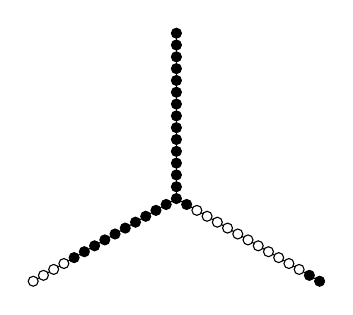
\begin{tikzpicture}[scale=.3]

\draw[color=black!100,thin] (0.000000,0.000000)--(0.000000,0.500000);
\draw[color=black!100,thin] (0.000000,0.500000)--(0.000000,1.000000);
\draw[color=black!100,thin] (0.000000,1.000000)--(0.000000,1.500000);
\draw[color=black!100,thin] (0.000000,1.500000)--(0.000000,2.000000);
\draw[color=black!100,thin] (0.000000,2.000000)--(0.000000,2.500000);
\draw[color=black!100,thin] (0.000000,2.500000)--(0.000000,3.000000);
\draw[color=black!100,thin] (0.000000,3.000000)--(0.000000,3.500000);
\draw[color=black!100,thin] (0.000000,3.500000)--(0.000000,4.000000);
\draw[color=black!100,thin] (0.000000,4.000000)--(0.000000,4.500000);
\draw[color=black!100,thin] (0.000000,4.500000)--(0.000000,5.000000);
\draw[color=black!100,thin] (0.000000,5.000000)--(0.000000,5.500000);
\draw[color=black!100,thin] (0.000000,5.500000)--(0.000000,6.000000);
\draw[color=black!100,thin] (0.000000,6.000000)--(0.000000,6.500000);
\draw[color=black!100,thin] (0.000000,6.500000)--(0.000000,7.000000);

\draw[color=black!100,thin] (0.000000,0.000000)--(-0.433013,-0.250000);
\draw[color=black!100,thin] (-0.433013,-0.250000)--(-0.866025,-0.500000);
\draw[color=black!100,thin] (-0.866025,-0.500000)--(-1.299038,-0.750000);
\draw[color=black!100,thin] (-1.299038,-0.750000)--(-1.732051,-1.000000);
\draw[color=black!100,thin] (-1.732051,-1.000000)--(-2.165064,-1.250000);
\draw[color=black!100,thin] (-2.165064,-1.250000)--(-2.598076,-1.500000);
\draw[color=black!100,thin] (-2.598076,-1.500000)--(-3.031089,-1.750000);
\draw[color=black!100,thin] (-3.031089,-1.750000)--(-3.464102,-2.000000);
\draw[color=black!100,thin] (-3.464102,-2.000000)--(-3.897114,-2.250000);
\draw[color=black!100,thin] (-3.897114,-2.250000)--(-4.330127,-2.500000);
\draw[color=black!100,thin] (-4.330127,-2.500000)--(-4.763140,-2.750000);
\draw[color=black!100,thin] (-4.763140,-2.750000)--(-5.196152,-3.000000);
\draw[color=black!100,thin] (-5.196152,-3.000000)--(-5.629165,-3.250000);
\draw[color=black!100,thin] (-5.629165,-3.250000)--(-6.062178,-3.500000);


\draw[color=black!100,thin] (0.000000,0.000000)--(0.433013,-0.250000);
\draw[color=black!100,thin] (0.433013,-0.250000)--(0.866025,-0.500000);
\draw[color=black!100,thin] (0.866025,-0.500000)--(1.299038,-0.750000);
\draw[color=black!100,thin] (1.299038,-0.750000)--(1.732051,-1.000000);
\draw[color=black!100,thin] (1.732051,-1.000000)--(2.165064,-1.250000);
\draw[color=black!100,thin] (2.165064,-1.250000)--(2.598076,-1.500000);
\draw[color=black!100,thin] (2.598076,-1.500000)--(3.031089,-1.750000);
\draw[color=black!100,thin] (3.031089,-1.750000)--(3.464102,-2.000000);
\draw[color=black!100,thin] (3.464102,-2.000000)--(3.897114,-2.250000);
\draw[color=black!100,thin] (3.897114,-2.250000)--(4.330127,-2.500000);
\draw[color=black!100,thin] (4.330127,-2.500000)--(4.763140,-2.750000);
\draw[color=black!100,thin] (4.763140,-2.750000)--(5.196152,-3.000000);
\draw[color=black!100,thin] (5.196152,-3.000000)--(5.629165,-3.250000);
\draw[color=black!100,thin] (5.629165,-3.250000)--(6.062178,-3.500000);


\draw[color=black!100,fill=black!100,thin] (0.000000,0.500000) circle (6.0pt);
\draw[color=black!100,fill=black!100,thin] (0.000000,1.000000) circle (6.0pt);
\draw[color=black!100,fill=black!100,thin] (0.000000,1.500000) circle (6.0pt);
\draw[color=black!100,fill=black!100,thin] (0.000000,2.000000) circle (6.0pt);
\draw[color=black!100,fill=black!100,thin] (0.000000,2.500000) circle (6.0pt);
\draw[color=black!100,fill=black!100,thin] (0.000000,3.000000) circle (6.0pt);
\draw[color=black!100,fill=black!100,thin] (0.000000,3.500000) circle (6.0pt);
\draw[color=black!100,fill=black!100,thin] (0.000000,4.000000) circle (6.0pt);
\draw[color=black!100,fill=black!100,thin] (0.000000,4.500000) circle (6.0pt);
\draw[color=black!100,fill=black!100,thin] (0.000000,5.000000) circle (6.0pt);
\draw[color=black!100,fill=black!100,thin] (0.000000,5.500000) circle (6.0pt);
\draw[color=black!100,fill=black!100,thin] (0.000000,6.000000) circle (6.0pt);
\draw[color=black!100,fill=black!100,thin] (0.000000,6.500000) circle (6.0pt);
\draw[color=black!100,fill=black!100,thin] (0.000000,7.000000) circle (6.0pt);



\draw[color=black!100,fill=black!100,thin] (0.433013,-0.250000) circle (6.0pt);
\draw[color=black!100,fill=black!0,thin] (0.866025,-0.500000) circle (6.0pt);
\draw[color=black!100,fill=black!0,thin] (1.299038,-0.750000) circle (6.0pt);
\draw[color=black!100,fill=black!0,thin] (1.732051,-1.000000) circle (6.0pt);
\draw[color=black!100,fill=black!0,thin] (2.165064,-1.250000) circle (6.0pt);
\draw[color=black!100,fill=black!0,thin] (2.598076,-1.500000) circle (6.0pt);
\draw[color=black!100,fill=black!0,thin] (3.031089,-1.750000) circle (6.0pt);
\draw[color=black!100,fill=black!0,thin] (3.464102,-2.000000) circle (6.0pt);
\draw[color=black!100,fill=black!0,thin] (3.897114,-2.250000) circle (6.0pt);
\draw[color=black!100,fill=black!0,thin] (4.330127,-2.500000) circle (6.0pt);
\draw[color=black!100,fill=black!0,thin] (4.763140,-2.750000) circle (6.0pt);
\draw[color=black!100,fill=black!0,thin] (5.196152,-3.000000) circle (6.0pt);
\draw[color=black!100,fill=black!100,thin] (5.629165,-3.250000) circle (6.0pt);
\draw[color=black!100,fill=black!100,thin] (6.062178,-3.500000) circle (6.0pt);




\draw[color=black!100,fill=black!100,thin] (-0.433013,-0.250000) circle (6.0pt);
\draw[color=black!100,fill=black!100,thin] (-0.866025,-0.500000) circle (6.0pt);
\draw[color=black!100,fill=black!100,thin] (-1.299038,-0.750000) circle (6.0pt);
\draw[color=black!100,fill=black!100,thin] (-1.732051,-1.000000) circle (6.0pt);
\draw[color=black!100,fill=black!100,thin] (-2.165064,-1.250000) circle (6.0pt);
\draw[color=black!100,fill=black!100,thin] (-2.598076,-1.500000) circle (6.0pt);
\draw[color=black!100,fill=black!100,thin] (-3.031089,-1.750000) circle (6.0pt);
\draw[color=black!100,fill=black!100,thin] (-3.464102,-2.000000) circle (6.0pt);
\draw[color=black!100,fill=black!100,thin] (-3.897114,-2.250000) circle (6.0pt);
\draw[color=black!100,fill=black!100,thin] (-4.330127,-2.500000) circle (6.0pt);
\draw[color=black!100,fill=black!0,thin] (-4.763140,-2.750000) circle (6.0pt);
\draw[color=black!100,fill=black!0,thin] (-5.196152,-3.000000) circle (6.0pt);
\draw[color=black!100,fill=black!0,thin] (-5.629165,-3.250000) circle (6.0pt);
\draw[color=black!100,fill=black!0,thin] (-6.062178,-3.500000) circle (6.0pt);


\draw[color=black!100,fill=black!100,thin] (0.000000,0.000000) circle (6.0pt);


\end{tikzpicture}
\end{subfigure}
\begin{subfigure}[b]{.4\textwidth}
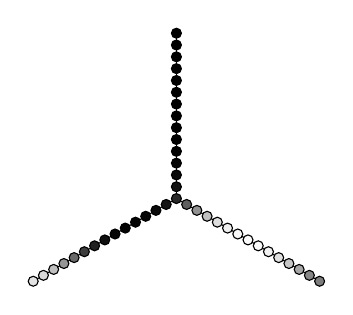
\begin{tikzpicture}[scale=.3]

\draw[color=black!100,thin] (0.000000,0.000000)--(0.000000,0.500000);
\draw[color=black!100,thin] (0.000000,0.500000)--(0.000000,1.000000);
\draw[color=black!100,thin] (0.000000,1.000000)--(0.000000,1.500000);
\draw[color=black!100,thin] (0.000000,1.500000)--(0.000000,2.000000);
\draw[color=black!100,thin] (0.000000,2.000000)--(0.000000,2.500000);
\draw[color=black!100,thin] (0.000000,2.500000)--(0.000000,3.000000);
\draw[color=black!100,thin] (0.000000,3.000000)--(0.000000,3.500000);
\draw[color=black!100,thin] (0.000000,3.500000)--(0.000000,4.000000);
\draw[color=black!100,thin] (0.000000,4.000000)--(0.000000,4.500000);
\draw[color=black!100,thin] (0.000000,4.500000)--(0.000000,5.000000);
\draw[color=black!100,thin] (0.000000,5.000000)--(0.000000,5.500000);
\draw[color=black!100,thin] (0.000000,5.500000)--(0.000000,6.000000);
\draw[color=black!100,thin] (0.000000,6.000000)--(0.000000,6.500000);
\draw[color=black!100,thin] (0.000000,6.500000)--(0.000000,7.000000);

\draw[color=black!100,thin] (0.000000,0.000000)--(-0.433013,-0.250000);
\draw[color=black!100,thin] (-0.433013,-0.250000)--(-0.866025,-0.500000);
\draw[color=black!100,thin] (-0.866025,-0.500000)--(-1.299038,-0.750000);
\draw[color=black!100,thin] (-1.299038,-0.750000)--(-1.732051,-1.000000);
\draw[color=black!100,thin] (-1.732051,-1.000000)--(-2.165064,-1.250000);
\draw[color=black!100,thin] (-2.165064,-1.250000)--(-2.598076,-1.500000);
\draw[color=black!100,thin] (-2.598076,-1.500000)--(-3.031089,-1.750000);
\draw[color=black!100,thin] (-3.031089,-1.750000)--(-3.464102,-2.000000);
\draw[color=black!100,thin] (-3.464102,-2.000000)--(-3.897114,-2.250000);
\draw[color=black!100,thin] (-3.897114,-2.250000)--(-4.330127,-2.500000);
\draw[color=black!100,thin] (-4.330127,-2.500000)--(-4.763140,-2.750000);
\draw[color=black!100,thin] (-4.763140,-2.750000)--(-5.196152,-3.000000);
\draw[color=black!100,thin] (-5.196152,-3.000000)--(-5.629165,-3.250000);
\draw[color=black!100,thin] (-5.629165,-3.250000)--(-6.062178,-3.500000);


\draw[color=black!100,thin] (0.000000,0.000000)--(0.433013,-0.250000);
\draw[color=black!100,thin] (0.433013,-0.250000)--(0.866025,-0.500000);
\draw[color=black!100,thin] (0.866025,-0.500000)--(1.299038,-0.750000);
\draw[color=black!100,thin] (1.299038,-0.750000)--(1.732051,-1.000000);
\draw[color=black!100,thin] (1.732051,-1.000000)--(2.165064,-1.250000);
\draw[color=black!100,thin] (2.165064,-1.250000)--(2.598076,-1.500000);
\draw[color=black!100,thin] (2.598076,-1.500000)--(3.031089,-1.750000);
\draw[color=black!100,thin] (3.031089,-1.750000)--(3.464102,-2.000000);
\draw[color=black!100,thin] (3.464102,-2.000000)--(3.897114,-2.250000);
\draw[color=black!100,thin] (3.897114,-2.250000)--(4.330127,-2.500000);
\draw[color=black!100,thin] (4.330127,-2.500000)--(4.763140,-2.750000);
\draw[color=black!100,thin] (4.763140,-2.750000)--(5.196152,-3.000000);
\draw[color=black!100,thin] (5.196152,-3.000000)--(5.629165,-3.250000);
\draw[color=black!100,thin] (5.629165,-3.250000)--(6.062178,-3.500000);


\draw[color=black!100,fill=black!92,thin] (0.000000,0.500000) circle (6.0pt);
\draw[color=black!100,fill=black!96,thin] (0.000000,1.000000) circle (6.0pt);
\draw[color=black!100,fill=black!99,thin] (0.000000,1.500000) circle (6.0pt);
\draw[color=black!100,fill=black!99,thin] (0.000000,2.000000) circle (6.0pt);
\draw[color=black!100,fill=black!100,thin] (0.000000,2.500000) circle (6.0pt);
\draw[color=black!100,fill=black!100,thin] (0.000000,3.000000) circle (6.0pt);
\draw[color=black!100,fill=black!100,thin] (0.000000,3.500000) circle (6.0pt);
\draw[color=black!100,fill=black!100,thin] (0.000000,4.000000) circle (6.0pt);
\draw[color=black!100,fill=black!100,thin] (0.000000,4.500000) circle (6.0pt);
\draw[color=black!100,fill=black!100,thin] (0.000000,5.000000) circle (6.0pt);
\draw[color=black!100,fill=black!100,thin] (0.000000,5.500000) circle (6.0pt);
\draw[color=black!100,fill=black!100,thin] (0.000000,6.000000) circle (6.0pt);
\draw[color=black!100,fill=black!100,thin] (0.000000,6.500000) circle (6.0pt);
\draw[color=black!100,fill=black!100,thin] (0.000000,7.000000) circle (6.0pt);

\draw[color=black!100,fill=black!63,thin] (0.433013,-0.250000) circle (6.0pt);
\draw[color=black!100,fill=black!43,thin] (0.866025,-0.500000) circle (6.0pt);
\draw[color=black!100,fill=black!25,thin] (1.299038,-0.750000) circle (6.0pt);
\draw[color=black!100,fill=black!13,thin] (1.732051,-1.000000) circle (6.0pt);
\draw[color=black!100,fill=black!6,thin] (2.165064,-1.250000) circle (6.0pt);
\draw[color=black!100,fill=black!2,thin] (2.598076,-1.500000) circle (6.0pt);
\draw[color=black!100,fill=black!2,thin] (3.031089,-1.750000) circle (6.0pt);
\draw[color=black!100,fill=black!2,thin] (3.464102,-2.000000) circle (6.0pt);
\draw[color=black!100,fill=black!5,thin] (3.897114,-2.250000) circle (6.0pt);
\draw[color=black!100,fill=black!12,thin] (4.330127,-2.500000) circle (6.0pt);
\draw[color=black!100,fill=black!22,thin] (4.763140,-2.750000) circle (6.0pt);
\draw[color=black!100,fill=black!35,thin] (5.196152,-3.000000) circle (6.0pt);
\draw[color=black!100,fill=black!47,thin] (5.629165,-3.250000) circle (6.0pt);
\draw[color=black!100,fill=black!51,thin] (6.062178,-3.500000) circle (6.0pt);

\draw[color=black!100,fill=black!92,thin] (-0.433013,-0.250000) circle (6.0pt);
\draw[color=black!100,fill=black!96,thin] (-0.866025,-0.500000) circle (6.0pt);
\draw[color=black!100,fill=black!98,thin] (-1.299038,-0.750000) circle (6.0pt);
\draw[color=black!100,fill=black!99,thin] (-1.732051,-1.000000) circle (6.0pt);
\draw[color=black!100,fill=black!99,thin] (-2.165064,-1.250000) circle (6.0pt);
\draw[color=black!100,fill=black!98,thin] (-2.598076,-1.500000) circle (6.0pt);
\draw[color=black!100,fill=black!94,thin] (-3.031089,-1.750000) circle (6.0pt);
\draw[color=black!100,fill=black!87,thin] (-3.464102,-2.000000) circle (6.0pt);
\draw[color=black!100,fill=black!76,thin] (-3.897114,-2.250000) circle (6.0pt);
\draw[color=black!100,fill=black!59,thin] (-4.330127,-2.500000) circle (6.0pt);
\draw[color=black!100,fill=black!41,thin] (-4.763140,-2.750000) circle (6.0pt);
\draw[color=black!100,fill=black!25,thin] (-5.196152,-3.000000) circle (6.0pt);
\draw[color=black!100,fill=black!15,thin] (-5.629165,-3.250000) circle (6.0pt);
\draw[color=black!100,fill=black!11,thin] (-6.062178,-3.500000) circle (6.0pt);

\draw[color=black!100,fill=black!84,thin] (0.000000,0.000000) circle (6.0pt);






\end{tikzpicture}
\end{subfigure}



\begin{figure}
    \centering
\begin{subfigure}[b]{.3\textwidth}
\input{tikz/ising/isingint1}
\end{subfigure}
\begin{subfigure}[b]{.3\textwidth}
\input{tikz/ising/isingcirc1}
\end{subfigure}
\begin{subfigure}[b]{.3\textwidth}
\documentclass{standalone}
\usepackage{xcolor}
\usepackage{tikz}
\usepackage{pgfplots}
\usepackage{pgfplots}
\usepgfplotslibrary{colormaps}
\pgfplotsset{compat=1.16}
\usetikzlibrary{positioning, backgrounds}

\input{figures/colmaps.tex}


\begin{document}

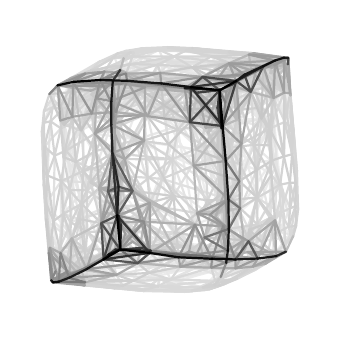
\begin{tikzpicture}[scale=.18]

\draw[color=white] (-10,-10) rectangle (10,10);

\draw[color=black!6,thick] (-4.366152,-1.509470)--(-6.225514,-2.397483);
\draw[color=black!6,thick] (-5.846316,-7.417451)--(-6.916578,-4.822716);
\draw[color=black!6,thick] (-4.135651,4.851512)--(-2.541217,6.610389);
\draw[color=black!6,thick] (-8.400703,-5.426916)--(-6.980125,-7.357355);
\draw[color=black!6,thick] (-5.709059,5.985034)--(-5.029043,6.534581);
\draw[color=black!6,thick] (3.897671,-1.489767)--(5.070391,-1.706943);
\draw[color=black!6,thick] (0.311620,-4.400587)--(-0.551283,-0.626135);
\draw[color=black!6,thick] (8.082185,-5.304309)--(7.490871,-6.080659);
\draw[color=black!6,thick] (5.044390,0.411375)--(3.966685,-2.325841);
\draw[color=black!6,thick] (-2.020294,6.429256)--(-2.541217,6.610389);
\draw[color=black!6,thick] (-5.182400,5.054698)--(-2.541217,6.610389);
\draw[color=black!6,thick] (-6.460221,6.681581)--(-7.757755,4.394611);
\draw[color=black!6,thick] (-3.900125,2.971452)--(-2.541217,6.610389);
\draw[color=black!6,thick] (-1.710627,-8.144912)--(-6.795680,-7.886239);
\draw[color=black!6,thick] (-5.594048,5.593107)--(-0.871136,5.284351);
\draw[color=black!6,thick] (-7.674359,-0.783184)--(-6.916578,-4.822716);
\draw[color=black!6,thick] (7.224593,-6.103934)--(8.687637,-4.682883);
\draw[color=black!6,thick] (5.542839,-5.032955)--(1.349867,-5.747199);
\draw[color=black!6,thick] (-4.911479,6.348369)--(-1.898006,3.965565);
\draw[color=black!6,thick] (6.904075,7.282142)--(6.657419,7.754539);
\draw[color=black!6,thick] (-3.624284,-1.181566)--(-1.830724,-3.644819);
\draw[color=black!6,thick] (4.737266,-6.121123)--(3.775698,-4.497221);
\draw[color=black!6,thick] (3.897671,-1.489767)--(4.634325,-4.913885);
\draw[color=black!6,thick] (3.643525,-6.971801)--(4.177013,-6.018543);
\draw[color=black!6,thick] (-4.456179,-0.340693)--(-6.756118,0.080987);
\draw[color=black!6,thick] (5.596656,-4.222627)--(4.177013,-6.018543);
\draw[color=black!6,thick] (-2.166375,6.620098)--(1.629286,5.992282);
\draw[color=black!6,thick] (1.671818,0.303518)--(4.287701,1.227531);
\draw[color=black!6,thick] (8.508169,5.257908)--(6.657419,7.754539);
\draw[color=black!6,thick] (-3.119225,8.399320)--(-1.718927,8.442384);
\draw[color=black!6,thick] (-4.991216,-1.269929)--(-4.263556,-1.303740);
\draw[color=black!6,thick] (-7.757755,4.394611)--(-7.002879,6.475108);
\draw[color=black!6,thick] (-8.735834,-2.335474)--(-8.546713,-5.872251);
\draw[color=black!6,thick] (-4.299745,-2.511956)--(-5.239168,1.334436);
\draw[color=black!6,thick] (7.224593,-6.103934)--(7.321363,-5.973787);
\draw[color=black!6,thick] (-8.903864,-1.049004)--(-8.546713,-5.872251);
\draw[color=black!6,thick] (-6.273599,2.786790)--(-7.726282,3.494291);
\draw[color=black!6,thick] (-4.031318,6.289935)--(-3.262951,7.879299);
\draw[color=black!6,thick] (7.055595,-3.378604)--(4.177013,-6.018543);
\draw[color=black!6,thick] (-5.940352,-8.035452)--(-8.476565,-5.488150);
\draw[color=black!6,thick] (-8.400703,-5.426916)--(-6.012983,-8.143566);
\draw[color=black!6,thick] (3.966685,-2.325841)--(5.070391,-1.706943);
\draw[color=black!6,thick] (-3.624284,-1.181566)--(-5.598493,-0.877305);
\draw[color=black!6,thick] (-2.166375,6.620098)--(-1.576849,3.797523);
\draw[color=black!6,thick] (-0.526488,5.717318)--(-0.399024,3.758035);
\draw[color=black!6,thick] (-4.299745,-2.511956)--(-6.756118,0.080987);
\draw[color=black!6,thick] (-8.504465,5.361578)--(-4.085111,5.189285);
\draw[color=black!6,thick] (6.124144,-1.942118)--(3.747086,-3.962405);
\draw[color=black!7,thick] (3.990455,-4.944430)--(1.765140,-3.863058);
\draw[color=black!7,thick] (-7.110700,-6.135776)--(-6.916578,-4.822716);
\draw[color=black!7,thick] (-6.698046,-7.751944)--(-6.980125,-7.357355);
\draw[color=black!7,thick] (-3.682076,8.225885)--(-5.570822,7.011715);
\draw[color=black!7,thick] (-7.171969,-7.144283)--(-5.940352,-8.035452);
\draw[color=black!7,thick] (1.906991,-3.045420)--(5.070391,-1.706943);
\draw[color=black!7,thick] (6.111328,8.045720)--(0.983446,8.369677);
\draw[color=black!7,thick] (5.294137,6.877908)--(5.883784,8.235279);
\draw[color=black!7,thick] (5.478520,-6.743434)--(7.415570,-3.552540);
\draw[color=black!7,thick] (-7.459705,3.178485)--(-7.002879,6.475108);
\draw[color=black!7,thick] (1.629286,5.992282)--(3.354619,4.382104);
\draw[color=black!7,thick] (1.801471,-6.899045)--(-1.469488,-7.263979);
\draw[color=black!7,thick] (-2.638285,-1.471882)--(-5.598493,-0.877305);
\draw[color=black!7,thick] (4.627007,-6.944348)--(4.326842,-7.717438);
\draw[color=black!7,thick] (7.059027,1.739309)--(7.055595,-3.378604);
\draw[color=black!7,thick] (2.827080,-3.157774)--(5.070391,-1.706943);
\draw[color=black!7,thick] (-6.698046,-7.751944)--(-8.476565,-5.488150);
\draw[color=black!7,thick] (-6.698046,-7.751944)--(-5.994808,-7.924081);
\draw[color=black!7,thick] (-3.185163,0.764786)--(-4.263556,-1.303740);
\draw[color=black!7,thick] (8.108130,5.639347)--(8.106534,3.390099);
\draw[color=black!7,thick] (1.629286,5.992282)--(1.999375,5.463559);
\draw[color=black!7,thick] (4.854351,7.674152)--(7.319221,5.081252);
\draw[color=black!7,thick] (-5.594048,5.593107)--(-2.099967,5.032639);
\draw[color=black!7,thick] (7.162750,7.218800)--(6.657419,7.754539);
\draw[color=black!7,thick] (-7.757755,4.394611)--(-5.709059,5.985034);
\draw[color=black!7,thick] (6.111328,8.045720)--(6.657419,7.754539);
\draw[color=black!7,thick] (-1.710627,-8.144912)--(1.716321,-8.447930);
\draw[color=black!7,thick] (2.827080,-3.157774)--(1.851669,1.423692);
\draw[color=black!7,thick] (-6.124383,-6.905994)--(-6.795680,-7.886239);
\draw[color=black!7,thick] (7.364702,7.395431)--(7.538546,5.733891);
\draw[color=black!7,thick] (-0.433729,7.663632)--(3.321173,6.363723);
\draw[color=black!7,thick] (-7.062663,-1.416283)--(-7.459705,3.178485);
\draw[color=black!7,thick] (3.966685,-2.325841)--(4.634325,-4.913885);
\draw[color=black!7,thick] (-4.018569,3.759294)--(-5.542522,5.323300);
\draw[color=black!7,thick] (-5.940352,-8.035452)--(-4.460532,-8.196229);
\draw[color=black!7,thick] (-0.433729,7.663632)--(-4.619582,6.945516);
\draw[color=black!7,thick] (1.629286,5.992282)--(4.822304,5.798717);
\draw[color=black!7,thick] (-0.526488,5.717318)--(0.996022,4.264888);
\draw[color=black!7,thick] (4.617552,-6.314066)--(7.490871,-6.080659);
\draw[color=black!7,thick] (-0.686857,6.847751)--(-0.399024,3.758035);
\draw[color=black!7,thick] (-3.027102,6.287395)--(-4.619582,6.945516);
\draw[color=black!7,thick] (-7.757755,4.394611)--(-8.889490,4.154151);
\draw[color=black!7,thick] (-4.456179,-0.340693)--(-6.273599,2.786790);
\draw[color=black!7,thick] (7.364702,7.395431)--(5.757018,7.018671);
\draw[color=black!7,thick] (5.542839,-5.032955)--(5.497874,-5.794872);
\draw[color=black!7,thick] (-2.276418,-6.574413)--(-2.580274,-7.824572);
\draw[color=black!7,thick] (-3.759113,4.109589)--(-5.900105,4.951972);
\draw[color=black!7,thick] (-3.338247,-8.169703)--(-0.460195,-6.709716);
\draw[color=black!7,thick] (7.364702,7.395431)--(5.971158,7.802493);
\draw[color=black!7,thick] (5.070391,-1.706943)--(4.634325,-4.913885);
\draw[color=black!7,thick] (-1.867682,-8.536631)--(-5.940352,-8.035452);
\draw[color=black!7,thick] (8.687637,-4.682883)--(7.415570,-3.552540);
\draw[color=black!7,thick] (-2.166375,6.620098)--(-3.465827,6.069730);
\draw[color=black!7,thick] (-5.594048,5.593107)--(-7.459705,3.178485);
\draw[color=black!7,thick] (3.643525,-6.971801)--(3.747086,-3.962405);
\draw[color=black!7,thick] (4.452409,6.894735)--(5.757018,7.018671);
\draw[color=black!7,thick] (-7.468452,5.082385)--(-5.542522,5.323300);
\draw[color=black!7,thick] (-6.460221,6.681581)--(-7.459705,3.178485);
\draw[color=black!7,thick] (7.364702,7.395431)--(8.106534,3.390099);
\draw[color=black!7,thick] (6.731622,-6.616961)--(5.596656,-4.222627);
\draw[color=black!7,thick] (-8.238916,-6.365989)--(-8.306212,-4.764287);
\draw[color=black!7,thick] (-1.423002,-2.317194)--(1.349867,-5.747199);
\draw[color=black!7,thick] (-6.698046,-7.751944)--(-8.070541,-7.154868);
\draw[color=black!7,thick] (-5.594048,5.593107)--(-7.757755,4.394611);
\draw[color=black!7,thick] (3.990455,-4.944430)--(5.542839,-5.032955);
\draw[color=black!7,thick] (7.490871,-6.080659)--(8.687637,-4.682883);
\draw[color=black!7,thick] (1.851669,1.423692)--(-2.455586,2.107211);
\draw[color=black!7,thick] (-8.546713,-5.872251)--(-5.940352,-8.035452);
\draw[color=black!7,thick] (5.397008,5.734684)--(8.074286,6.434098);
\draw[color=black!7,thick] (7.059027,1.739309)--(7.929146,-1.391529);
\draw[color=black!7,thick] (-3.682076,8.225885)--(-6.460221,6.681581);
\draw[color=black!7,thick] (-6.326810,-6.210033)--(-8.546713,-5.872251);
\draw[color=black!7,thick] (6.446009,3.620490)--(6.155795,-1.954461);
\draw[color=black!7,thick] (-1.201643,6.785879)--(3.321173,6.363723);
\draw[color=black!7,thick] (0.996022,4.264888)--(1.999375,5.463559);
\draw[color=black!7,thick] (5.757018,7.018671)--(7.538546,5.733891);
\draw[color=black!7,thick] (-7.829593,-5.649701)--(-8.306212,-4.764287);
\draw[color=black!7,thick] (2.445606,6.376712)--(6.592800,7.331144);
\draw[color=black!7,thick] (8.108130,5.639347)--(7.162750,7.218800);
\draw[color=black!7,thick] (-8.579828,-4.918894)--(-7.015604,-7.274615);
\draw[color=black!7,thick] (-7.838650,-7.882261)--(-8.238916,-6.365989);
\draw[color=black!7,thick] (-4.373557,-5.636691)--(-4.263556,-1.303740);
\draw[color=black!7,thick] (-7.015604,-7.274615)--(-5.940352,-8.035452);
\draw[color=black!7,thick] (5.542839,-5.032955)--(1.765140,-3.863058);
\draw[color=black!7,thick] (8.900997,-3.955079)--(7.321363,-5.973787);
\draw[color=black!7,thick] (-1.576849,3.797523)--(0.996022,4.264888);
\draw[color=black!7,thick] (-5.900105,4.951972)--(-7.545654,4.308500);
\draw[color=black!7,thick] (-8.400703,-5.426916)--(-7.015604,-7.274615);
\draw[color=black!7,thick] (-7.838650,-7.882261)--(-8.218875,-3.606144);
\draw[color=black!7,thick] (-2.166375,6.620098)--(-3.822581,4.082228);
\draw[color=black!7,thick] (8.508330,-4.544313)--(7.321363,-5.973787);
\draw[color=black!7,thick] (4.627007,-6.944348)--(3.747086,-3.962405);
\draw[color=black!7,thick] (2.827080,-3.157774)--(4.085932,-5.689507);
\draw[color=black!7,thick] (-4.018569,3.759294)--(-2.636161,5.158663);
\draw[color=black!7,thick] (-3.262951,7.879299)--(-2.541217,6.610389);
\draw[color=black!7,thick] (7.775901,-1.038829)--(7.207088,4.918943);
\draw[color=black!7,thick] (5.596656,-4.222627)--(2.908839,-6.892003);
\draw[color=black!7,thick] (3.935372,0.638063)--(2.827080,-3.157774);
\draw[color=black!7,thick] (8.074286,6.434098)--(5.392431,6.323172);
\draw[color=black!7,thick] (-5.994808,-7.924081)--(-8.476565,-5.488150);
\draw[color=black!7,thick] (-3.759113,4.109589)--(-1.763127,6.211371);
\draw[color=black!7,thick] (-2.652046,7.998916)--(-3.101780,6.793060);
\draw[color=black!7,thick] (-1.830724,-3.644819)--(0.162370,0.756226);
\draw[color=black!7,thick] (3.966685,-2.325841)--(1.883179,-5.940374);
\draw[color=black!7,thick] (-3.822581,4.082228)--(-0.399024,3.758035);
\draw[color=black!7,thick] (-5.709059,5.985034)--(-7.002879,6.475108);
\draw[color=black!7,thick] (5.497874,-5.794872)--(7.055595,-3.378604);
\draw[color=black!7,thick] (-8.752960,-3.488356)--(-7.224567,-7.160908);
\draw[color=black!7,thick] (3.643525,-6.971801)--(1.349867,-5.747199);
\draw[color=black!7,thick] (-0.123497,-5.152358)--(4.166451,-5.383936);
\draw[color=black!7,thick] (3.896234,1.588448)--(0.996022,4.264888);
\draw[color=black!7,thick] (8.108130,5.639347)--(5.883784,8.235279);
\draw[color=black!7,thick] (4.737266,-6.121123)--(1.883179,-5.940374);
\draw[color=black!7,thick] (3.200807,-3.301946)--(2.827080,-3.157774);
\draw[color=black!7,thick] (-6.326810,-6.210033)--(-8.476565,-5.488150);
\draw[color=black!7,thick] (-0.433729,7.663632)--(1.114993,8.423620);
\draw[color=black!7,thick] (-3.900125,2.971452)--(-2.636161,5.158663);
\draw[color=black!7,thick] (-6.827710,6.213818)--(-3.936667,4.855694);
\draw[color=black!7,thick] (-7.468452,5.082385)--(-4.692746,6.449616);
\draw[color=black!7,thick] (5.254429,6.724045)--(4.854351,7.674152);
\draw[color=black!7,thick] (3.990455,-4.944430)--(0.607928,-6.162136);
\draw[color=black!7,thick] (2.324529,-8.286781)--(3.643525,-6.971801);
\draw[color=black!7,thick] (5.397008,5.734684)--(3.616575,5.202755);
\draw[color=black!8,thick] (-8.070541,-7.154868)--(-7.224567,-7.160908);
\draw[color=black!8,thick] (-3.936667,4.855694)--(0.996022,4.264888);
\draw[color=black!8,thick] (-1.830724,-3.644819)--(-1.469488,-7.263979);
\draw[color=black!8,thick] (-5.972366,6.797337)--(-3.465827,6.069730);
\draw[color=black!8,thick] (-3.822581,4.082228)--(-1.898006,3.965565);
\draw[color=black!8,thick] (-3.936667,4.855694)--(-0.619826,6.106975);
\draw[color=black!8,thick] (-1.201643,6.785879)--(-4.419299,7.244964);
\draw[color=black!8,thick] (-6.698046,-7.751944)--(-7.015604,-7.274615);
\draw[color=black!8,thick] (-0.433729,7.663632)--(4.854351,7.674152);
\draw[color=black!8,thick] (-3.624284,-1.181566)--(-1.423002,-2.317194);
\draw[color=black!8,thick] (-8.504465,5.361578)--(-7.459705,3.178485);
\draw[color=black!8,thick] (2.760017,-5.896365)--(5.854381,-6.818046);
\draw[color=black!8,thick] (3.614034,3.467925)--(-1.788224,3.882865);
\draw[color=black!8,thick] (8.687637,-4.682883)--(4.166451,-5.383936);
\draw[color=black!8,thick] (-7.124115,-6.304288)--(-6.124383,-6.905994);
\draw[color=black!8,thick] (3.562342,0.061988)--(0.996022,4.264888);
\draw[color=black!8,thick] (4.159352,7.526481)--(-0.686857,6.847751);
\draw[color=black!8,thick] (-0.753634,-7.657461)--(-3.903752,-8.343434);
\draw[color=black!8,thick] (2.445606,6.376712)--(3.321173,6.363723);
\draw[color=black!8,thick] (5.971158,7.802493)--(5.883784,8.235279);
\draw[color=black!8,thick] (-2.276418,-6.574413)--(2.908839,-6.892003);
\draw[color=black!8,thick] (8.074286,6.434098)--(8.806098,1.826392);
\draw[color=black!8,thick] (3.896234,1.588448)--(1.481362,5.846428);
\draw[color=black!8,thick] (1.671818,0.303518)--(-0.399024,3.758035);
\draw[color=black!8,thick] (-3.902475,-0.009340)--(-3.448784,-3.886943);
\draw[color=black!8,thick] (-1.763127,6.211371)--(-3.900125,2.971452);
\draw[color=black!8,thick] (5.702919,5.505272)--(2.513011,2.979092);
\draw[color=black!8,thick] (-0.830720,-8.199291)--(-0.460195,-6.709716);
\draw[color=black!8,thick] (7.775901,-1.038829)--(4.954710,-2.700410);
\draw[color=black!8,thick] (-5.182400,5.054698)--(-2.636161,5.158663);
\draw[color=black!8,thick] (3.200807,-3.301946)--(5.001278,-5.980424);
\draw[color=black!8,thick] (7.153944,-0.341147)--(5.596656,-4.222627);
\draw[color=black!8,thick] (-8.546713,-5.872251)--(-6.980125,-7.357355);
\draw[color=black!8,thick] (-3.900125,2.971452)--(-3.448784,-3.886943);
\draw[color=black!8,thick] (-7.171969,-7.144283)--(-8.400703,-5.426916);
\draw[color=black!8,thick] (7.207088,4.918943)--(8.053171,7.922610);
\draw[color=black!8,thick] (-8.238916,-6.365989)--(-6.012983,-8.143566);
\draw[color=black!8,thick] (-8.929860,-0.071208)--(-8.400703,-5.426916);
\draw[color=black!8,thick] (-7.110700,-6.135776)--(-6.251431,-7.055464);
\draw[color=black!8,thick] (-6.122213,-0.079723)--(-4.770036,-2.975602);
\draw[color=black!8,thick] (-4.619582,6.945516)--(-0.686857,6.847751);
\draw[color=black!8,thick] (-3.759113,4.109589)--(-2.541217,6.610389);
\draw[color=black!8,thick] (4.854351,7.674152)--(1.114993,8.423620);
\draw[color=black!8,thick] (3.562342,0.061988)--(4.085932,-5.689507);
\draw[color=black!8,thick] (1.801471,-6.899045)--(-2.580274,-7.824572);
\draw[color=black!8,thick] (5.044390,0.411375)--(7.216269,0.672411);
\draw[color=black!8,thick] (3.200807,-3.301946)--(0.311620,-4.400587);
\draw[color=black!8,thick] (4.309947,1.589199)--(7.153944,-0.341147);
\draw[color=black!8,thick] (-0.830720,-8.199291)--(1.801471,-6.899045);
\draw[color=black!8,thick] (7.085149,6.820039)--(4.822304,5.798717);
\draw[color=black!8,thick] (1.801471,-6.899045)--(3.747086,-3.962405);
\draw[color=black!8,thick] (7.364702,7.395431)--(5.254429,6.724045);
\draw[color=black!8,thick] (6.904075,7.282142)--(7.538546,5.733891);
\draw[color=black!8,thick] (6.057132,6.960897)--(7.538546,5.733891);
\draw[color=black!8,thick] (-3.262951,7.879299)--(-2.020294,6.429256);
\draw[color=black!8,thick] (4.452409,6.894735)--(1.999375,5.463559);
\draw[color=black!8,thick] (-6.827710,6.213818)--(-1.201643,6.785879);
\draw[color=black!8,thick] (-6.460221,6.681581)--(-5.029043,6.534581);
\draw[color=black!8,thick] (-4.018569,3.759294)--(-1.763127,6.211371);
\draw[color=black!8,thick] (-4.373557,-5.636691)--(-6.980125,-7.357355);
\draw[color=black!8,thick] (-7.171969,-7.144283)--(-8.579828,-4.918894);
\draw[color=black!8,thick] (-0.830720,-8.199291)--(-5.994808,-7.924081);
\draw[color=black!8,thick] (-2.541217,6.610389)--(-1.718927,8.442384);
\draw[color=black!8,thick] (6.904075,7.282142)--(8.108130,5.639347);
\draw[color=black!8,thick] (-2.276418,-6.574413)--(-0.325915,-5.683992);
\draw[color=black!8,thick] (-8.903864,-1.049004)--(-8.306212,-4.764287);
\draw[color=black!8,thick] (-7.269627,-6.318021)--(-8.306212,-4.764287);
\draw[color=black!8,thick] (4.724253,3.530405)--(6.446009,3.620490);
\draw[color=black!8,thick] (-1.763127,6.211371)--(3.616575,5.202755);
\draw[color=black!8,thick] (-4.018569,3.759294)--(-3.750271,0.009945);
\draw[color=black!8,thick] (4.890212,-0.788773)--(2.827080,-3.157774);
\draw[color=black!8,thick] (3.562342,0.061988)--(-0.399024,3.758035);
\draw[color=black!8,thick] (4.164610,8.331563)--(0.983446,8.369677);
\draw[color=black!8,thick] (4.724253,3.530405)--(1.629286,5.992282);
\draw[color=black!8,thick] (1.629286,5.992282)--(1.399345,3.369483);
\draw[color=black!8,thick] (-4.018569,3.759294)--(-3.845303,0.558062);
\draw[color=black!8,thick] (-6.698046,-7.751944)--(-5.846316,-7.417451);
\draw[color=black!8,thick] (-6.246043,-5.560379)--(-3.338247,-8.169703);
\draw[color=black!8,thick] (-1.755632,5.829931)--(-5.401249,4.277229);
\draw[color=black!8,thick] (-7.548844,-2.876630)--(-6.756118,0.080987);
\draw[color=black!8,thick] (-1.422134,-5.854065)--(-0.325915,-5.683992);
\draw[color=black!8,thick] (1.671818,0.303518)--(-2.455586,2.107211);
\draw[color=black!8,thick] (-1.755632,5.829931)--(-4.692746,6.449616);
\draw[color=black!8,thick] (-0.012133,4.556084)--(3.616575,5.202755);
\draw[color=black!8,thick] (1.349867,-5.747199)--(-1.469488,-7.263979);
\draw[color=black!8,thick] (5.569266,8.136105)--(7.538546,5.733891);
\draw[color=black!8,thick] (6.446009,3.620490)--(4.676247,6.279021);
\draw[color=black!8,thick] (4.954710,-2.700410)--(7.216269,0.672411);
\draw[color=black!8,thick] (4.890212,-0.788773)--(6.446009,3.620490);
\draw[color=black!8,thick] (2.445606,6.376712)--(-0.871136,5.284351);
\draw[color=black!8,thick] (5.569266,8.136105)--(8.108130,5.639347);
\draw[color=black!8,thick] (-1.830724,-3.644819)--(-3.448784,-3.886943);
\draw[color=black!8,thick] (3.458876,7.323677)--(7.418012,7.724718);
\draw[color=black!8,thick] (4.890212,-0.788773)--(7.216269,0.672411);
\draw[color=black!8,thick] (7.079030,0.972315)--(7.415570,-3.552540);
\draw[color=black!8,thick] (-0.753634,-7.657461)--(2.324529,-8.286781);
\draw[color=black!8,thick] (-6.246043,-5.560379)--(-4.460532,-8.196229);
\draw[color=black!8,thick] (-3.185163,0.764786)--(-3.900125,2.971452);
\draw[color=black!8,thick] (5.299006,7.359558)--(7.319221,5.081252);
\draw[color=black!8,thick] (-0.830720,-8.199291)--(3.643525,-6.971801);
\draw[color=black!8,thick] (1.671818,0.303518)--(5.044390,0.411375);
\draw[color=black!8,thick] (8.074286,6.434098)--(8.348709,7.909134);
\draw[color=black!8,thick] (-7.171969,-7.144283)--(-6.698046,-7.751944);
\draw[color=black!8,thick] (-2.541217,6.610389)--(-4.692746,6.449616);
\draw[color=black!8,thick] (-8.579828,-4.918894)--(-6.795680,-7.886239);
\draw[color=black!8,thick] (4.452409,6.894735)--(6.057132,6.960897);
\draw[color=black!8,thick] (-6.460221,6.681581)--(-5.709059,5.985034);
\draw[color=black!8,thick] (0.996022,4.264888)--(2.306670,6.565949);
\draw[color=black!8,thick] (7.224593,-6.103934)--(7.415570,-3.552540);
\draw[color=black!8,thick] (4.452409,6.894735)--(5.702919,5.505272);
\draw[color=black!8,thick] (-8.579828,-4.918894)--(-8.306212,-4.764287);
\draw[color=black!8,thick] (-1.755632,5.829931)--(-3.165044,2.056806);
\draw[color=black!8,thick] (-3.750271,0.009945)--(-3.251855,-1.990655);
\draw[color=black!8,thick] (-3.750271,0.009945)--(-1.788224,3.882865);
\draw[color=black!8,thick] (-1.763127,6.211371)--(2.328527,4.988791);
\draw[color=black!8,thick] (5.596656,-4.222627)--(3.747086,-3.962405);
\draw[color=black!8,thick] (8.108130,5.639347)--(8.616865,1.105019);
\draw[color=black!8,thick] (2.335451,-6.068067)--(-0.460195,-6.709716);
\draw[color=black!8,thick] (-3.485414,-0.603218)--(-4.770036,-2.975602);
\draw[color=black!8,thick] (3.696543,6.269186)--(3.616575,5.202755);
\draw[color=black!8,thick] (-4.849991,-3.754716)--(-4.263556,-1.303740);
\draw[color=black!8,thick] (7.364702,7.395431)--(4.159352,7.526481);
\draw[color=black!8,thick] (3.983171,5.529157)--(1.042957,5.776546);
\draw[color=black!8,thick] (2.513011,2.979092)--(-0.871136,5.284351);
\draw[color=black!8,thick] (3.967222,-6.554432)--(4.634325,-4.913885);
\draw[color=black!8,thick] (7.224593,-6.103934)--(5.854381,-6.818046);
\draw[color=black!8,thick] (-5.972366,6.797337)--(-5.029043,6.534581);
\draw[color=black!8,thick] (5.478520,-6.743434)--(4.326842,-7.717438);
\draw[color=black!8,thick] (5.043500,1.853477)--(6.155795,-1.954461);
\draw[color=black!8,thick] (-7.224567,-7.160908)--(-6.980125,-7.357355);
\draw[color=black!8,thick] (5.044390,0.411375)--(6.125036,-0.000818);
\draw[color=black!8,thick] (4.890212,-0.788773)--(4.524157,-3.171849);
\draw[color=black!8,thick] (-0.399024,3.758035)--(2.306670,6.565949);
\draw[color=black!8,thick] (3.896234,1.588448)--(3.718852,3.100078);
\draw[color=black!8,thick] (-6.698046,-7.751944)--(-8.546713,-5.872251);
\draw[color=black!8,thick] (-5.182400,5.054698)--(-1.763127,6.211371);
\draw[color=black!8,thick] (-7.721392,-5.860722)--(-3.772463,-7.404603);
\draw[color=black!8,thick] (5.971158,7.802493)--(5.757018,7.018671);
\draw[color=black!8,thick] (-2.297414,-4.346011)--(2.442317,-4.764951);
\draw[color=black!8,thick] (-3.900125,2.971452)--(-4.692746,6.449616);
\draw[color=black!8,thick] (-6.367602,-3.477821)--(-5.598493,-0.877305);
\draw[color=black!8,thick] (5.478520,-6.743434)--(5.596656,-4.222627);
\draw[color=black!8,thick] (-1.423002,-2.317194)--(0.546657,2.829928);
\draw[color=black!8,thick] (-5.594048,5.593107)--(-6.827710,6.213818);
\draw[color=black!8,thick] (-7.110700,-6.135776)--(-6.980125,-7.357355);
\draw[color=black!8,thick] (3.896234,1.588448)--(3.200807,-3.301946);
\draw[color=black!8,thick] (-4.770036,-2.975602)--(-4.341375,-5.975923);
\draw[color=black!8,thick] (-5.972366,6.797337)--(-7.757755,4.394611);
\draw[color=black!8,thick] (6.057132,6.960897)--(2.445606,6.376712);
\draw[color=black!8,thick] (-3.750271,0.009945)--(-4.770036,-2.975602);
\draw[color=black!8,thick] (-3.900125,2.971452)--(-5.542522,5.323300);
\draw[color=black!8,thick] (-3.759113,4.109589)--(-3.262951,7.879299);
\draw[color=black!8,thick] (-5.401249,4.277229)--(-3.900125,2.971452);
\draw[color=black!8,thick] (5.044390,0.411375)--(7.022498,2.913922);
\draw[color=black!8,thick] (3.990455,-4.944430)--(2.908839,-6.892003);
\draw[color=black!8,thick] (4.954710,-2.700410)--(4.634325,-4.913885);
\draw[color=black!8,thick] (2.680487,2.609783)--(3.966685,-2.325841);
\draw[color=black!8,thick] (5.294137,6.877908)--(1.629286,5.992282);
\draw[color=black!8,thick] (0.546657,2.829928)--(1.765140,-3.863058);
\draw[color=black!8,thick] (7.224593,-6.103934)--(5.497874,-5.794872);
\draw[color=black!8,thick] (-1.928914,-5.490566)--(-1.830724,-3.644819);
\draw[color=black!8,thick] (7.364702,7.395431)--(8.108130,5.639347);
\draw[color=black!8,thick] (7.793554,-3.021585)--(5.203977,-4.955209);
\draw[color=black!8,thick] (2.335451,-6.068067)--(3.643525,-6.971801);
\draw[color=black!8,thick] (8.477380,5.428594)--(6.657419,7.754539);
\draw[color=black!8,thick] (-3.465827,6.069730)--(-3.936667,4.855694);
\draw[color=black!8,thick] (6.446009,3.620490)--(3.718852,3.100078);
\draw[color=black!8,thick] (-7.468452,5.082385)--(-8.176810,5.284919);
\draw[color=black!8,thick] (-1.819668,2.076325)--(-5.304397,2.557643);
\draw[color=black!8,thick] (6.446009,3.620490)--(8.043051,0.956032);
\draw[color=black!8,thick] (-4.849991,-3.754716)--(-3.185163,0.764786);
\draw[color=black!8,thick] (8.053171,7.922610)--(4.854351,7.674152);
\draw[color=black!8,thick] (-6.246043,-5.560379)--(-3.903752,-8.343434);
\draw[color=black!8,thick] (4.287701,1.227531)--(4.524157,-3.171849);
\draw[color=black!8,thick] (-8.752960,-3.488356)--(-8.218875,-3.606144);
\draw[color=black!8,thick] (-0.012133,4.556084)--(-4.135651,4.851512);
\draw[color=black!8,thick] (-3.465827,6.069730)--(-5.029043,6.534581);
\draw[color=black!8,thick] (-7.015604,-7.274615)--(-8.238916,-6.365989);
\draw[color=black!8,thick] (6.111328,8.045720)--(7.364702,7.395431);
\draw[color=black!8,thick] (5.043500,1.853477)--(2.513011,2.979092);
\draw[color=black!8,thick] (6.904075,7.282142)--(5.971158,7.802493);
\draw[color=black!9,thick] (-1.788224,3.882865)--(-2.636161,5.158663);
\draw[color=black!9,thick] (3.643525,-6.971801)--(0.051276,-7.724115);
\draw[color=black!9,thick] (4.724253,3.530405)--(7.022498,2.913922);
\draw[color=black!9,thick] (4.676247,6.279021)--(5.757018,7.018671);
\draw[color=black!9,thick] (5.299006,7.359558)--(4.159352,7.526481);
\draw[color=black!9,thick] (-8.892133,3.325055)--(-8.176810,5.284919);
\draw[color=black!9,thick] (-7.757755,4.394611)--(-4.815010,5.896649);
\draw[color=black!9,thick] (-7.331712,1.364334)--(-5.598493,-0.877305);
\draw[color=black!9,thick] (3.990455,-4.944430)--(6.197657,-6.250126);
\draw[color=black!9,thick] (-3.845303,0.558062)--(-5.304397,2.557643);
\draw[color=black!9,thick] (-1.063548,-2.549232)--(2.442317,-4.764951);
\draw[color=black!9,thick] (3.983171,5.529157)--(3.479088,3.511400);
\draw[color=black!9,thick] (-5.972366,6.797337)--(-6.273599,2.786790);
\draw[color=black!9,thick] (8.508169,5.257908)--(8.108130,5.639347);
\draw[color=black!9,thick] (6.904075,7.282142)--(5.757018,7.018671);
\draw[color=black!9,thick] (-3.772463,-7.404603)--(-6.367602,-3.477821);
\draw[color=black!9,thick] (-1.788224,3.882865)--(-1.423002,-2.317194);
\draw[color=black!9,thick] (4.287701,1.227531)--(1.399345,3.369483);
\draw[color=black!9,thick] (4.890212,-0.788773)--(7.022498,2.913922);
\draw[color=black!9,thick] (5.478520,-6.743434)--(3.198996,-7.822990);
\draw[color=black!9,thick] (6.111328,8.045720)--(8.074286,6.434098);
\draw[color=black!9,thick] (4.452409,6.894735)--(4.676247,6.279021);
\draw[color=black!9,thick] (-3.750271,0.009945)--(-5.304397,2.557643);
\draw[color=black!9,thick] (-1.898006,3.965565)--(1.042957,5.776546);
\draw[color=black!9,thick] (-3.338247,-8.169703)--(-6.251431,-7.055464);
\draw[color=black!9,thick] (-1.898006,3.965565)--(-0.686857,6.847751);
\draw[color=black!9,thick] (-1.755632,5.829931)--(3.616575,5.202755);
\draw[color=black!9,thick] (-6.698046,-7.751944)--(-6.124383,-6.905994);
\draw[color=black!9,thick] (-5.972366,6.797337)--(-1.201643,6.785879);
\draw[color=black!9,thick] (-6.827710,6.213818)--(-7.726282,3.494291);
\draw[color=black!9,thick] (-1.830724,-3.644819)--(-3.848843,-5.612673);
\draw[color=black!9,thick] (-6.460221,6.681581)--(-4.986561,7.632262);
\draw[color=black!9,thick] (2.513011,2.979092)--(3.479088,3.511400);
\draw[color=black!9,thick] (-2.276418,-6.574413)--(-1.423002,-2.317194);
\draw[color=black!9,thick] (-1.763127,6.211371)--(-4.692746,6.449616);
\draw[color=black!9,thick] (3.896234,1.588448)--(-0.399024,3.758035);
\draw[color=black!9,thick] (5.195668,6.845604)--(6.657419,7.754539);
\draw[color=black!9,thick] (-7.545654,4.308500)--(-5.542522,5.323300);
\draw[color=black!9,thick] (0.256401,-1.841582)--(0.546657,2.829928);
\draw[color=black!9,thick] (8.478040,-2.712398)--(7.688754,-4.368218);
\draw[color=black!9,thick] (-8.400703,-5.426916)--(-8.657224,-0.386164);
\draw[color=black!9,thick] (-4.849991,-3.754716)--(-1.423002,-2.317194);
\draw[color=black!9,thick] (-3.448784,-3.886943)--(-3.845303,0.558062);
\draw[color=black!9,thick] (6.197657,-6.250126)--(2.966201,-6.266712);
\draw[color=black!9,thick] (0.726931,-6.828657)--(-2.580274,-7.824572);
\draw[color=black!9,thick] (-8.579828,-4.918894)--(-8.903864,-1.049004);
\draw[color=black!9,thick] (-8.238916,-6.365989)--(-8.476565,-5.488150);
\draw[color=black!9,thick] (7.538546,5.733891)--(7.319221,5.081252);
\draw[color=black!9,thick] (-3.750271,0.009945)--(-4.031318,6.289935);
\draw[color=black!9,thick] (6.111328,8.045720)--(7.689004,6.695515);
\draw[color=black!9,thick] (4.452409,6.894735)--(2.445606,6.376712);
\draw[color=black!9,thick] (-7.331712,1.364334)--(-6.225514,-2.397483);
\draw[color=black!9,thick] (-4.815010,5.896649)--(-6.273599,2.786790);
\draw[color=black!9,thick] (2.827080,-3.157774)--(-0.551283,-0.626135);
\draw[color=black!9,thick] (3.896234,1.588448)--(5.043500,1.853477);
\draw[color=black!9,thick] (6.468890,4.400624)--(7.541488,0.277664);
\draw[color=black!9,thick] (6.904075,7.282142)--(8.106534,3.390099);
\draw[color=black!9,thick] (-1.469488,-7.263979)--(2.908839,-6.892003);
\draw[color=black!9,thick] (7.364702,7.395431)--(6.657419,7.754539);
\draw[color=black!9,thick] (-5.846316,-7.417451)--(-6.251431,-7.055464);
\draw[color=black!9,thick] (3.897671,-1.489767)--(4.524157,-3.171849);
\draw[color=black!9,thick] (-0.526488,5.717318)--(-3.822581,4.082228);
\draw[color=black!9,thick] (-5.994808,-7.924081)--(-7.110700,-6.135776);
\draw[color=black!9,thick] (4.159352,7.526481)--(7.022498,2.913922);
\draw[color=black!9,thick] (-3.822581,4.082228)--(-1.201643,6.785879);
\draw[color=black!9,thick] (8.053034,5.444800)--(5.971158,7.802493);
\draw[color=black!9,thick] (-0.460195,-6.709716)--(2.966201,-6.266712);
\draw[color=black!9,thick] (3.321173,6.363723)--(7.319221,5.081252);
\draw[color=black!9,thick] (-3.822581,4.082228)--(-5.709059,5.985034);
\draw[color=black!9,thick] (5.299006,7.359558)--(5.254429,6.724045);
\draw[color=black!9,thick] (-0.460195,-6.709716)--(0.051276,-7.724115);
\draw[color=black!9,thick] (3.896234,1.588448)--(5.702919,5.505272);
\draw[color=black!9,thick] (-0.085890,1.804660)--(1.851669,1.423692);
\draw[color=black!9,thick] (-5.401249,4.277229)--(-7.698633,2.935231);
\draw[color=black!9,thick] (-1.830724,-3.644819)--(-0.460195,-6.709716);
\draw[color=black!9,thick] (-6.109553,3.679259)--(-5.900105,4.951972);
\draw[color=black!9,thick] (-1.423002,-2.317194)--(-3.845303,0.558062);
\draw[color=black!9,thick] (-6.460221,6.681581)--(-4.419299,7.244964);
\draw[color=black!9,thick] (5.294137,6.877908)--(2.306670,6.565949);
\draw[color=black!9,thick] (-2.297414,-4.346011)--(1.883179,-5.940374);
\draw[color=black!9,thick] (3.458876,7.323677)--(2.925294,8.019294);
\draw[color=black!9,thick] (7.207088,4.918943)--(5.702919,5.505272);
\draw[color=black!9,thick] (-8.735834,-2.335474)--(-6.246043,-5.560379);
\draw[color=black!9,thick] (3.321173,6.363723)--(7.022498,2.913922);
\draw[color=black!9,thick] (4.309947,1.589199)--(0.162370,0.756226);
\draw[color=black!9,thick] (6.124144,-1.942118)--(7.541488,0.277664);
\draw[color=black!9,thick] (-4.139673,3.209598)--(-5.598493,-0.877305);
\draw[color=black!9,thick] (-1.763127,6.211371)--(1.370377,6.070440);
\draw[color=black!9,thick] (-0.012133,4.556084)--(-1.763127,6.211371);
\draw[color=black!9,thick] (-6.698046,-7.751944)--(-6.012983,-8.143566);
\draw[color=black!9,thick] (4.724253,3.530405)--(3.647158,2.935537);
\draw[color=black!9,thick] (-0.433729,7.663632)--(-0.686857,6.847751);
\draw[color=black!9,thick] (-5.846316,-7.417451)--(-3.772463,-7.404603);
\draw[color=black!9,thick] (-7.459705,3.178485)--(-6.642516,0.559893);
\draw[color=black!9,thick] (-6.916578,-4.822716)--(-5.598493,-0.877305);
\draw[color=black!9,thick] (1.969665,8.540591)--(5.883784,8.235279);
\draw[color=black!9,thick] (4.724253,3.530405)--(5.294137,6.877908);
\draw[color=black!9,thick] (-7.721392,-5.860722)--(-7.674359,-0.783184);
\draw[color=black!9,thick] (-7.171969,-7.144283)--(-6.980125,-7.357355);
\draw[color=black!9,thick] (-7.721392,-5.860722)--(-8.258154,-7.932871);
\draw[color=black!9,thick] (-3.759113,4.109589)--(-5.542522,5.323300);
\draw[color=black!9,thick] (-7.721392,-5.860722)--(-6.367602,-3.477821);
\draw[color=black!9,thick] (-4.619582,6.945516)--(-6.273599,2.786790);
\draw[color=black!9,thick] (-0.433729,7.663632)--(2.306670,6.565949);
\draw[color=black!9,thick] (-0.433729,7.663632)--(-4.419299,7.244964);
\draw[color=black!9,thick] (-7.171969,-7.144283)--(-8.238916,-6.365989);
\draw[color=black!9,thick] (-0.399024,3.758035)--(1.042957,5.776546);
\draw[color=black!9,thick] (-8.735834,-2.335474)--(-8.400703,-5.426916);
\draw[color=black!9,thick] (-3.903752,-8.343434)--(-5.940352,-8.035452);
\draw[color=black!9,thick] (-3.027102,6.287395)--(0.996022,4.264888);
\draw[color=black!9,thick] (5.043500,1.853477)--(1.851669,1.423692);
\draw[color=black!9,thick] (-4.815010,5.896649)--(-7.459705,3.178485);
\draw[color=black!9,thick] (-3.822581,4.082228)--(-6.273599,2.786790);
\draw[color=black!9,thick] (-6.795680,-7.886239)--(-8.238916,-6.365989);
\draw[color=black!9,thick] (4.452409,6.894735)--(4.159352,7.526481);
\draw[color=black!9,thick] (-5.846316,-7.417451)--(-6.980125,-7.357355);
\draw[color=black!9,thick] (-1.576849,3.797523)--(-1.201643,6.785879);
\draw[color=black!9,thick] (1.020131,-8.602831)--(-1.772853,-8.455876);
\draw[color=black!9,thick] (4.159352,7.526481)--(7.319221,5.081252);
\draw[color=black!9,thick] (-3.509456,7.052040)--(-1.718927,8.442384);
\draw[color=black!9,thick] (3.588510,-7.540642)--(3.378896,-8.222676);
\draw[color=black!9,thick] (7.055595,-3.378604)--(5.854381,-6.818046);
\draw[color=black!9,thick] (-6.246043,-5.560379)--(-8.218875,-3.606144);
\draw[color=black!9,thick] (-0.460195,-6.709716)--(-2.580274,-7.824572);
\draw[color=black!9,thick] (-3.101780,6.793060)--(1.042957,5.776546);
\draw[color=black!9,thick] (-7.124115,-6.304288)--(-7.027945,-5.286674);
\draw[color=black!9,thick] (-3.772463,-7.404603)--(-6.225514,-2.397483);
\draw[color=black!9,thick] (-1.755632,5.829931)--(-5.542522,5.323300);
\draw[color=black!9,thick] (4.890212,-0.788773)--(4.287701,1.227531);
\draw[color=black!9,thick] (5.001278,-5.980424)--(6.174623,-3.841037);
\draw[color=black!9,thick] (1.765140,-3.863058)--(2.404414,1.717320);
\draw[color=black!9,thick] (7.364702,7.395431)--(5.294137,6.877908);
\draw[color=black!9,thick] (1.399345,3.369483)--(-2.455586,2.107211);
\draw[color=black!9,thick] (-6.698046,-7.751944)--(-6.795680,-7.886239);
\draw[color=black!9,thick] (6.904075,7.282142)--(4.724253,3.530405);
\draw[color=black!9,thick] (-5.709059,5.985034)--(-7.726282,3.494291);
\draw[color=black!9,thick] (3.321173,6.363723)--(-0.686857,6.847751);
\draw[color=black!9,thick] (5.910650,1.769356)--(7.541488,0.277664);
\draw[color=black!9,thick] (6.446009,3.620490)--(3.321173,6.363723);
\draw[color=black!9,thick] (-1.201643,6.785879)--(-4.815010,5.896649);
\draw[color=black!9,thick] (-2.952717,5.532537)--(-5.709059,5.985034);
\draw[color=black!9,thick] (-5.594048,5.593107)--(-6.460221,6.681581);
\draw[color=black!9,thick] (-3.465827,6.069730)--(-6.273599,2.786790);
\draw[color=black!9,thick] (-3.907434,7.903094)--(-3.509456,7.052040);
\draw[color=black!9,thick] (3.200807,-3.301946)--(1.906991,-3.045420);
\draw[color=black!9,thick] (-0.686857,6.847751)--(2.925294,8.019294);
\draw[color=black!10,thick] (5.910650,1.769356)--(7.055595,-3.378604);
\draw[color=black!10,thick] (3.896234,1.588448)--(2.680487,2.609783);
\draw[color=black!10,thick] (-5.846316,-7.417451)--(-7.721392,-5.860722);
\draw[color=black!10,thick] (3.616575,5.202755)--(1.370377,6.070440);
\draw[color=black!10,thick] (4.164610,8.331563)--(2.925294,8.019294);
\draw[color=black!10,thick] (8.687637,-4.682883)--(7.929146,-1.391529);
\draw[color=black!10,thick] (4.309947,1.589199)--(3.747086,-3.962405);
\draw[color=black!10,thick] (-6.251431,-7.055464)--(-3.848843,-5.612673);
\draw[color=black!10,thick] (-8.579828,-4.918894)--(-8.929860,-0.071208);
\draw[color=black!10,thick] (3.747086,-3.962405)--(2.404414,1.717320);
\draw[color=black!10,thick] (-6.980125,-7.357355)--(-3.848843,-5.612673);
\draw[color=black!10,thick] (-1.201643,6.785879)--(3.458876,7.323677);
\draw[color=black!10,thick] (-0.156487,8.666513)--(-2.561622,8.273109);
\draw[color=black!10,thick] (6.446009,3.620490)--(5.254429,6.724045);
\draw[color=black!10,thick] (5.702919,5.505272)--(2.445606,6.376712);
\draw[color=black!10,thick] (-1.201643,6.785879)--(1.399345,3.369483);
\draw[color=black!10,thick] (6.904075,7.282142)--(7.319221,5.081252);
\draw[color=black!10,thick] (5.569266,8.136105)--(5.294137,6.877908);
\draw[color=black!10,thick] (-5.838167,-4.362183)--(-6.756118,0.080987);
\draw[color=black!10,thick] (-2.020294,6.429256)--(-5.542522,5.323300);
\draw[color=black!10,thick] (-7.000444,-3.698639)--(-4.299745,-2.511956);
\draw[color=black!10,thick] (-3.101780,6.793060)--(0.295150,8.005740);
\draw[color=black!10,thick] (-6.367602,-3.477821)--(-7.331712,1.364334);
\draw[color=black!10,thick] (3.966685,-2.325841)--(4.524157,-3.171849);
\draw[color=black!10,thick] (-6.698046,-7.751944)--(-7.224567,-7.160908);
\draw[color=black!10,thick] (3.903135,4.771999)--(1.042957,5.776546);
\draw[color=black!10,thick] (-2.166375,6.620098)--(-5.029043,6.534581);
\draw[color=black!10,thick] (2.513011,2.979092)--(3.354619,4.382104);
\draw[color=black!10,thick] (4.123332,-2.075159)--(1.851669,1.423692);
\draw[color=black!10,thick] (3.354619,4.382104)--(2.306670,6.565949);
\draw[color=black!10,thick] (-4.991216,-1.269929)--(-1.423002,-2.317194);
\draw[color=black!10,thick] (8.174537,-5.769804)--(7.541488,0.277664);
\draw[color=black!10,thick] (-1.710627,-8.144912)--(-1.867682,-8.536631);
\draw[color=black!10,thick] (7.216269,0.672411)--(7.319221,5.081252);
\draw[color=black!10,thick] (-8.400703,-5.426916)--(-8.218875,-3.606144);
\draw[color=black!10,thick] (-7.721392,-5.860722)--(-5.866616,-6.989533);
\draw[color=black!10,thick] (5.299006,7.359558)--(3.458876,7.323677);
\draw[color=black!10,thick] (3.983171,5.529157)--(1.999375,5.463559);
\draw[color=black!10,thick] (-6.246043,-5.560379)--(-8.752960,-3.488356);
\draw[color=black!10,thick] (-3.907434,7.903094)--(-4.986561,7.632262);
\draw[color=black!10,thick] (-8.657224,-0.386164)--(-8.476565,-5.488150);
\draw[color=black!10,thick] (7.207088,4.918943)--(7.216269,0.672411);
\draw[color=black!10,thick] (-5.972366,6.797337)--(-7.459705,3.178485);
\draw[color=black!10,thick] (-5.304397,2.557643)--(-4.770036,-2.975602);
\draw[color=black!10,thick] (-0.526488,5.717318)--(-0.686857,6.847751);
\draw[color=black!10,thick] (4.166451,-5.383936)--(4.177013,-6.018543);
\draw[color=black!10,thick] (4.724253,3.530405)--(4.890212,-0.788773);
\draw[color=black!10,thick] (-6.367602,-3.477821)--(-6.251431,-7.055464);
\draw[color=black!10,thick] (6.057132,6.960897)--(1.481362,5.846428);
\draw[color=black!10,thick] (2.335451,-6.068067)--(1.801471,-6.899045);
\draw[color=black!10,thick] (7.364702,7.395431)--(7.319221,5.081252);
\draw[color=black!10,thick] (-5.994808,-7.924081)--(-7.224567,-7.160908);
\draw[color=black!10,thick] (-3.509456,7.052040)--(1.370377,6.070440);
\draw[color=black!10,thick] (-5.513480,3.975774)--(-5.029043,6.534581);
\draw[color=black!10,thick] (-1.830724,-3.644819)--(-3.185163,0.764786);
\draw[color=black!10,thick] (-5.709059,5.985034)--(-6.883179,3.745660);
\draw[color=black!10,thick] (3.643525,-6.971801)--(3.198996,-7.822990);
\draw[color=black!10,thick] (-8.903864,-1.049004)--(-9.033835,2.718915);
\draw[color=black!10,thick] (2.445606,6.376712)--(2.513011,2.979092);
\draw[color=black!10,thick] (4.500326,-2.105728)--(0.162370,0.756226);
\draw[color=black!10,thick] (-6.795680,-7.886239)--(-8.306212,-4.764287);
\draw[color=black!10,thick] (-7.000444,-3.698639)--(-6.756118,0.080987);
\draw[color=black!10,thick] (-7.468452,5.082385)--(-5.900105,4.951972);
\draw[color=black!10,thick] (5.392431,6.323172)--(3.616575,5.202755);
\draw[color=black!10,thick] (4.737266,-6.121123)--(5.001278,-5.980424);
\draw[color=black!10,thick] (6.057132,6.960897)--(4.854351,7.674152);
\draw[color=black!10,thick] (-7.511225,0.906399)--(-6.756118,0.080987);
\draw[color=black!10,thick] (-7.062663,-1.416283)--(-6.756118,0.080987);
\draw[color=black!10,thick] (-5.864677,-1.436696)--(-6.756118,0.080987);
\draw[color=black!10,thick] (-7.459705,3.178485)--(-6.756118,0.080987);
\draw[color=black!10,thick] (-6.273599,2.786790)--(-6.756118,0.080987);
\draw[color=black!10,thick] (-6.642516,0.559893)--(-6.756118,0.080987);
\draw[color=black!10,thick] (-6.883179,3.745660)--(-6.756118,0.080987);
\draw[color=black!10,thick] (-5.239168,1.334436)--(-6.756118,0.080987);
\draw[color=black!10,thick] (-7.726282,3.494291)--(-6.756118,0.080987);
\filldraw[color=black!10] (-6.756118,0.080987) circle (1.000000pt);
\draw[color=black!10,thick] (-0.651153,5.670028)--(1.851669,1.423692);
\draw[color=black!10,thick] (3.647158,2.935537)--(6.446009,3.620490);
\draw[color=black!10,thick] (5.043500,1.853477)--(4.287701,1.227531);
\draw[color=black!10,thick] (-5.401249,4.277229)--(-7.331712,1.364334);
\draw[color=black!10,thick] (-7.224567,-7.160908)--(-8.238916,-6.365989);
\draw[color=black!10,thick] (1.906991,-3.045420)--(4.524157,-3.171849);
\draw[color=black!10,thick] (-1.755632,5.829931)--(-2.541217,6.610389);
\draw[color=black!10,thick] (-7.757755,4.394611)--(-7.726282,3.494291);
\draw[color=black!10,thick] (-6.623057,4.788217)--(-7.331712,1.364334);
\draw[color=black!10,thick] (-3.185163,0.764786)--(-1.788224,3.882865);
\draw[color=black!10,thick] (8.508330,-4.544313)--(7.688754,-4.368218);
\draw[color=black!10,thick] (6.174623,-3.841037)--(2.442317,-4.764951);
\draw[color=black!10,thick] (5.044390,0.411375)--(3.718852,3.100078);
\draw[color=black!10,thick] (-6.827710,6.213818)--(-3.101780,6.793060);
\draw[color=black!10,thick] (-1.710627,-8.144912)--(-4.460532,-8.196229);
\draw[color=black!10,thick] (-1.710627,-8.144912)--(-0.890117,-8.457960);
\filldraw[color=black!10] (-1.710627,-8.144912) circle (1.000000pt);
\draw[color=black!10,thick] (-3.101780,6.793060)--(-5.029043,6.534581);
\draw[color=black!10,thick] (-1.423002,-2.317194)--(-4.770036,-2.975602);
\draw[color=black!10,thick] (7.207088,4.918943)--(8.043051,0.956032);
\draw[color=black!10,thick] (4.634325,-4.913885)--(2.442317,-4.764951);
\draw[color=black!10,thick] (-6.122213,-0.079723)--(-6.367602,-3.477821);
\draw[color=black!10,thick] (5.569266,8.136105)--(8.477380,5.428594);
\draw[color=black!10,thick] (4.412024,6.044017)--(2.445606,6.376712);
\draw[color=black!10,thick] (6.111328,8.045720)--(7.085149,6.820039);
\draw[color=black!10,thick] (4.452409,6.894735)--(4.854351,7.674152);
\draw[color=black!10,thick] (7.224593,-6.103934)--(6.197657,-6.250126);
\draw[color=black!10,thick] (-4.341375,-5.975923)--(-6.980125,-7.357355);
\draw[color=black!10,thick] (-6.246043,-5.560379)--(-8.546713,-5.872251);
\draw[color=black!10,thick] (-3.822581,4.082228)--(-0.686857,6.847751);
\draw[color=black!10,thick] (8.082185,-5.304309)--(7.321363,-5.973787);
\draw[color=black!10,thick] (-2.635362,-5.059762)--(-3.609696,-3.241754);
\draw[color=black!10,thick] (-0.433729,7.663632)--(-0.764599,8.471513);
\draw[color=black!10,thick] (-6.795680,-7.886239)--(-7.015604,-7.274615);
\draw[color=black!10,thick] (5.757018,7.018671)--(5.254429,6.724045);
\draw[color=black!10,thick] (5.883784,8.235279)--(6.657419,7.754539);
\draw[color=black!10,thick] (3.966685,-2.325841)--(3.476895,-1.005757);
\draw[color=black!10,thick] (4.954710,-2.700410)--(4.085932,-5.689507);
\draw[color=black!10,thick] (-7.529767,-3.097927)--(-5.598493,-0.877305);
\draw[color=black!10,thick] (-0.764599,8.471513)--(-2.844154,7.460024);
\draw[color=black!10,thick] (-3.149159,-4.504206)--(-1.355665,-5.699041);
\draw[color=black!10,thick] (-0.012133,4.556084)--(-4.018569,3.759294);
\draw[color=black!10,thick] (0.674086,-8.335090)--(-0.890117,-8.457960);
\draw[color=black!10,thick] (3.966685,-2.325841)--(1.399345,3.369483);
\draw[color=black!10,thick] (4.724253,3.530405)--(7.319221,5.081252);
\draw[color=black!10,thick] (-5.542522,5.323300)--(-7.698633,2.935231);
\draw[color=black!10,thick] (-1.819668,2.076325)--(-3.750271,0.009945);
\draw[color=black!10,thick] (6.124144,-1.942118)--(6.197657,-6.250126);
\draw[color=black!10,thick] (8.508169,5.257908)--(5.883784,8.235279);
\draw[color=black!10,thick] (8.074286,6.434098)--(5.195668,6.845604);
\draw[color=black!10,thick] (-0.873345,7.424582)--(2.306670,6.565949);
\draw[color=black!10,thick] (7.224593,-6.103934)--(5.478520,-6.743434);
\draw[color=black!11,thick] (-3.450209,1.410202)--(-3.251855,-1.990655);
\draw[color=black!11,thick] (-0.433729,7.663632)--(2.925294,8.019294);
\draw[color=black!11,thick] (4.822304,5.798717)--(3.903135,4.771999);
\draw[color=black!11,thick] (5.299006,7.359558)--(6.057132,6.960897);
\draw[color=black!11,thick] (3.990455,-4.944430)--(2.335451,-6.068067);
\draw[color=black!11,thick] (-0.686857,6.847751)--(1.481362,5.846428);
\draw[color=black!11,thick] (-1.763127,6.211371)--(-1.788224,3.882865);
\draw[color=black!11,thick] (2.827080,-3.157774)--(4.524157,-3.171849);
\draw[color=black!11,thick] (-1.755632,5.829931)--(-2.636161,5.158663);
\draw[color=black!11,thick] (-7.929580,5.967579)--(-8.176810,5.284919);
\draw[color=black!11,thick] (-1.063548,-2.549232)--(-2.455586,2.107211);
\draw[color=black!11,thick] (6.446009,3.620490)--(4.159352,7.526481);
\draw[color=black!11,thick] (1.399345,3.369483)--(3.354619,4.382104);
\draw[color=black!11,thick] (3.479088,3.511400)--(2.306670,6.565949);
\draw[color=black!11,thick] (-1.819668,2.076325)--(-3.900125,2.971452);
\draw[color=black!11,thick] (8.053171,7.922610)--(5.757018,7.018671);
\draw[color=black!11,thick] (-3.101780,6.793060)--(-5.709059,5.985034);
\draw[color=black!11,thick] (5.043500,1.853477)--(4.123332,-2.075159);
\draw[color=black!11,thick] (0.162370,0.756226)--(1.765140,-3.863058);
\draw[color=black!11,thick] (-0.873345,7.424582)--(-4.619582,6.945516);
\draw[color=black!11,thick] (6.731622,-6.616961)--(5.478520,-6.743434);
\draw[color=black!11,thick] (4.737266,-6.121123)--(3.588510,-7.540642);
\draw[color=black!11,thick] (-2.276418,-6.574413)--(-3.448784,-3.886943);
\draw[color=black!11,thick] (-7.511225,0.906399)--(-6.273599,2.786790);
\draw[color=black!11,thick] (5.203977,-4.955209)--(4.634325,-4.913885);
\draw[color=black!11,thick] (-3.772463,-7.404603)--(-0.460195,-6.709716);
\draw[color=black!11,thick] (-0.433729,7.663632)--(-3.101780,6.793060);
\draw[color=black!11,thick] (-3.101780,6.793060)--(-1.576849,3.797523);
\draw[color=black!11,thick] (-2.635362,-5.059762)--(-4.341375,-5.975923);
\draw[color=black!11,thick] (-5.937659,-5.621537)--(-6.124383,-6.905994);
\draw[color=black!11,thick] (-8.070541,-7.154868)--(-6.124383,-6.905994);
\draw[color=black!11,thick] (-6.124383,-6.905994)--(-7.269627,-6.318021);
\draw[color=black!11,thick] (-6.124383,-6.905994)--(-8.376926,-7.790421);
\draw[color=black!11,thick] (-6.124383,-6.905994)--(-4.341650,-5.575292);
\filldraw[color=black!11] (-6.124383,-6.905994) circle (1.000000pt);
\draw[color=black!11,thick] (-4.849991,-3.754716)--(-1.928914,-5.490566);
\draw[color=black!11,thick] (2.445606,6.376712)--(1.399345,3.369483);
\draw[color=black!11,thick] (-2.635362,-5.059762)--(-0.123497,-5.152358);
\draw[color=black!11,thick] (5.757018,7.018671)--(7.022498,2.913922);
\draw[color=black!11,thick] (7.272080,3.662058)--(7.541488,0.277664);
\draw[color=black!11,thick] (-0.753634,-7.657461)--(-0.830720,-8.199291);
\draw[color=black!11,thick] (-0.085890,1.804660)--(-0.399024,3.758035);
\draw[color=black!11,thick] (7.055595,-3.378604)--(7.541488,0.277664);
\draw[color=black!11,thick] (-2.276418,-6.574413)--(-3.848843,-5.612673);
\draw[color=black!11,thick] (4.676247,6.279021)--(0.996022,4.264888);
\draw[color=black!11,thick] (-3.902475,-0.009340)--(-3.485414,-0.603218);
\draw[color=black!11,thick] (5.043500,1.853477)--(7.319221,5.081252);
\draw[color=black!11,thick] (7.207088,4.918943)--(7.022498,2.913922);
\draw[color=black!11,thick] (-1.201643,6.785879)--(-0.651153,5.670028);
\draw[color=black!11,thick] (-3.902475,-0.009340)--(-5.598493,-0.877305);
\draw[color=black!11,thick] (-5.994808,-7.924081)--(-6.916578,-4.822716);
\draw[color=black!11,thick] (-0.433729,7.663632)--(3.458876,7.323677);
\draw[color=black!11,thick] (4.617552,-6.314066)--(1.349867,-5.747199);
\draw[color=black!11,thick] (-1.576849,3.797523)--(-0.551283,-0.626135);
\draw[color=black!11,thick] (6.027726,-7.043482)--(7.321363,-5.973787);
\draw[color=black!11,thick] (4.724253,3.530405)--(1.399345,3.369483);
\draw[color=black!11,thick] (5.195668,6.845604)--(4.421133,5.564371);
\draw[color=black!11,thick] (-7.721392,-5.860722)--(-7.224567,-7.160908);
\draw[color=black!11,thick] (5.927481,5.663480)--(5.195668,6.845604);
\draw[color=black!11,thick] (5.397008,5.734684)--(5.195668,6.845604);
\draw[color=black!11,thick] (5.195668,6.845604)--(3.696543,6.269186);
\draw[color=black!11,thick] (5.195668,6.845604)--(5.392431,6.323172);
\draw[color=black!11,thick] (5.195668,6.845604)--(7.007128,5.847543);
\draw[color=black!11,thick] (5.195668,6.845604)--(7.689004,6.695515);
\draw[color=black!11,thick] (5.195668,6.845604)--(8.323893,7.461020);
\filldraw[color=black!11] (5.195668,6.845604) circle (1.000000pt);
\draw[color=black!11,thick] (8.508169,5.257908)--(7.085149,6.820039);
\draw[color=black!11,thick] (1.999375,5.463559)--(3.903135,4.771999);
\draw[color=black!11,thick] (6.057132,6.960897)--(6.446009,3.620490);
\draw[color=black!11,thick] (-4.135651,4.851512)--(-3.902475,-0.009340);
\draw[color=black!11,thick] (4.737266,-6.121123)--(5.203977,-4.955209);
\draw[color=black!11,thick] (7.079030,0.972315)--(7.272080,3.662058);
\draw[color=black!11,thick] (-5.972366,6.797337)--(-5.709059,5.985034);
\draw[color=black!11,thick] (8.082185,-5.304309)--(8.900997,-3.955079);
\draw[color=black!11,thick] (-8.735834,-2.335474)--(-8.579828,-4.918894);
\draw[color=black!11,thick] (5.043500,1.853477)--(3.966685,-2.325841);
\draw[color=black!11,thick] (-2.276418,-6.574413)--(-4.770036,-2.975602);
\draw[color=black!11,thick] (-7.002879,6.475108)--(-4.986561,7.632262);
\draw[color=black!11,thick] (-1.201643,6.785879)--(-5.709059,5.985034);
\draw[color=black!11,thick] (2.324529,-8.286781)--(0.051276,-7.724115);
\draw[color=black!11,thick] (-5.513480,3.975774)--(-2.455586,2.107211);
\draw[color=black!11,thick] (-8.425381,3.434168)--(-8.657224,-0.386164);
\draw[color=black!11,thick] (3.588510,-7.540642)--(-0.004614,-6.112553);
\draw[color=black!11,thick] (7.415570,-3.552540)--(4.177013,-6.018543);
\draw[color=black!11,thick] (-2.276418,-6.574413)--(-3.609696,-3.241754);
\draw[color=black!11,thick] (-6.460221,6.681581)--(-4.006072,7.915461);
\draw[color=black!11,thick] (-3.101780,6.793060)--(-3.936667,4.855694);
\draw[color=black!11,thick] (-5.994808,-7.924081)--(-1.772853,-8.455876);
\draw[color=black!11,thick] (-7.757755,4.394611)--(-6.883179,3.745660);
\draw[color=black!11,thick] (-8.579828,-4.918894)--(-8.070541,-7.154868);
\draw[color=black!11,thick] (-6.460221,6.681581)--(-4.619582,6.945516);
\draw[color=black!11,thick] (8.082185,-5.304309)--(7.224593,-6.103934);
\draw[color=black!11,thick] (-1.355665,-5.699041)--(1.765140,-3.863058);
\draw[color=black!11,thick] (-6.246043,-5.560379)--(-6.012983,-8.143566);
\draw[color=black!11,thick] (-0.433729,7.663632)--(-1.201643,6.785879);
\draw[color=black!11,thick] (6.468890,4.400624)--(3.616575,5.202755);
\draw[color=black!11,thick] (1.629286,5.992282)--(1.042957,5.776546);
\draw[color=black!11,thick] (6.111328,8.045720)--(2.644286,8.168361);
\draw[color=black!11,thick] (-1.423002,-2.317194)--(-4.680085,-6.305119);
\draw[color=black!11,thick] (-7.721392,-5.860722)--(-7.110700,-6.135776);
\draw[color=black!11,thick] (3.200807,-3.301946)--(5.203977,-4.955209);
\draw[color=black!11,thick] (0.674086,-8.335090)--(2.324529,-8.286781);
\draw[color=black!11,thick] (-8.735834,-2.335474)--(-7.674359,-0.783184);
\draw[color=black!11,thick] (-3.149159,-4.504206)--(-4.341375,-5.975923);
\draw[color=black!11,thick] (7.079030,0.972315)--(7.541488,0.277664);
\draw[color=black!11,thick] (7.153944,-0.341147)--(7.541488,0.277664);
\draw[color=black!11,thick] (7.059027,1.739309)--(7.541488,0.277664);
\draw[color=black!11,thick] (7.929146,-1.391529)--(7.541488,0.277664);
\draw[color=black!11,thick] (7.541488,0.277664)--(7.415570,-3.552540);
\filldraw[color=black!11] (7.541488,0.277664) circle (1.000000pt);
\draw[color=black!11,thick] (1.801471,-6.899045)--(0.051276,-7.724115);
\draw[color=black!11,thick] (3.359146,1.237080)--(3.966685,-2.325841);
\draw[color=black!11,thick] (-5.594048,5.593107)--(-7.002879,6.475108);
\draw[color=black!11,thick] (2.335451,-6.068067)--(5.497874,-5.794872);
\draw[color=black!11,thick] (-8.579828,-4.918894)--(-8.752960,-3.488356);
\draw[color=black!11,thick] (-6.460221,6.681581)--(-7.726282,3.494291);
\draw[color=black!11,thick] (3.718852,3.100078)--(-0.651153,5.670028);
\draw[color=black!11,thick] (2.335451,-6.068067)--(-1.423002,-2.317194);
\draw[color=black!11,thick] (0.607928,-6.162136)--(2.908839,-6.892003);
\draw[color=black!11,thick] (3.647158,2.935537)--(2.513011,2.979092);
\draw[color=black!11,thick] (8.508169,5.257908)--(7.364702,7.395431);
\draw[color=black!11,thick] (7.207088,4.918943)--(6.057132,6.960897);
\draw[color=black!11,thick] (-0.619826,6.106975)--(1.573697,7.248827);
\draw[color=black!11,thick] (-3.822581,4.082228)--(-4.619582,6.945516);
\draw[color=black!11,thick] (4.287701,1.227531)--(5.070391,-1.706943);
\draw[color=black!11,thick] (-6.251431,-7.055464)--(-0.460195,-6.709716);
\draw[color=black!11,thick] (-3.750271,0.009945)--(-1.423002,-2.317194);
\draw[color=black!12,thick] (-5.864677,-1.436696)--(-6.273599,2.786790);
\draw[color=black!12,thick] (4.287701,1.227531)--(4.123332,-2.075159);
\draw[color=black!12,thick] (6.111328,8.045720)--(7.162750,7.218800);
\draw[color=black!12,thick] (-4.849991,-3.754716)--(-3.772463,-7.404603);
\draw[color=black!12,thick] (-1.422134,-5.854065)--(1.349867,-5.747199);
\draw[color=black!12,thick] (-0.686857,6.847751)--(1.399345,3.369483);
\draw[color=black!12,thick] (-4.849991,-3.754716)--(-3.750271,0.009945);
\draw[color=black!12,thick] (3.897671,-1.489767)--(1.399345,3.369483);
\draw[color=black!12,thick] (8.323893,7.461020)--(6.657419,7.754539);
\draw[color=black!12,thick] (-0.526488,5.717318)--(2.445606,6.376712);
\draw[color=black!12,thick] (-3.822581,4.082228)--(-3.936667,4.855694);
\draw[color=black!12,thick] (7.207088,4.918943)--(8.108130,5.639347);
\draw[color=black!12,thick] (5.854381,-6.818046)--(4.177013,-6.018543);
\draw[color=black!12,thick] (-0.460195,-6.709716)--(-4.680085,-6.305119);
\draw[color=black!12,thick] (5.542839,-5.032955)--(5.478520,-6.743434);
\draw[color=black!12,thick] (-5.513480,3.975774)--(-3.101780,6.793060);
\draw[color=black!12,thick] (-8.857305,1.651783)--(-7.698633,2.935231);
\draw[color=black!12,thick] (-7.721392,-5.860722)--(-6.246043,-5.560379);
\draw[color=black!12,thick] (-6.246043,-5.560379)--(-7.838650,-7.882261);
\draw[color=black!12,thick] (-6.246043,-5.560379)--(-5.994808,-7.924081);
\draw[color=black!12,thick] (-6.246043,-5.560379)--(-8.258154,-7.932871);
\draw[color=black!12,thick] (-6.246043,-5.560379)--(-7.224567,-7.160908);
\draw[color=black!12,thick] (-6.246043,-5.560379)--(-8.476565,-5.488150);
\filldraw[color=black!12] (-6.246043,-5.560379) circle (1.000000pt);
\draw[color=black!12,thick] (-4.263556,-1.303740)--(-4.341375,-5.975923);
\draw[color=black!12,thick] (-1.830724,-3.644819)--(-4.770036,-2.975602);
\draw[color=black!12,thick] (-1.355665,-5.699041)--(-1.423002,-2.317194);
\draw[color=black!12,thick] (6.028613,6.589774)--(6.057132,6.960897);
\draw[color=black!12,thick] (5.203977,-4.955209)--(6.155795,-1.954461);
\draw[color=black!12,thick] (1.567526,-8.537910)--(3.475711,-8.150895);
\draw[color=black!12,thick] (1.765140,-3.863058)--(2.908839,-6.892003);
\draw[color=black!12,thick] (-6.367602,-3.477821)--(-7.674359,-0.783184);
\draw[color=black!12,thick] (-0.753634,-7.657461)--(-0.890117,-8.457960);
\draw[color=black!12,thick] (5.299006,7.359558)--(5.971158,7.802493);
\draw[color=black!12,thick] (-7.110700,-6.135776)--(-5.866616,-6.989533);
\draw[color=black!12,thick] (7.153944,-0.341147)--(7.055595,-3.378604);
\draw[color=black!12,thick] (2.513011,2.979092)--(3.903135,4.771999);
\draw[color=black!12,thick] (3.967222,-6.554432)--(-0.004614,-6.112553);
\draw[color=black!12,thick] (0.726931,-6.828657)--(-1.830724,-3.644819);
\draw[color=black!12,thick] (5.542839,-5.032955)--(2.966201,-6.266712);
\draw[color=black!12,thick] (-7.674359,-0.783184)--(-5.598493,-0.877305);
\draw[color=black!12,thick] (0.295150,8.005740)--(-0.686857,6.847751);
\draw[color=black!12,thick] (5.971158,7.802493)--(6.657419,7.754539);
\draw[color=black!12,thick] (4.737266,-6.121123)--(4.634325,-4.913885);
\draw[color=black!12,thick] (-7.511225,0.906399)--(-7.459705,3.178485);
\draw[color=black!12,thick] (5.044390,0.411375)--(4.287701,1.227531);
\draw[color=black!12,thick] (-0.526488,5.717318)--(2.513011,2.979092);
\draw[color=black!12,thick] (0.256401,-1.841582)--(2.404414,1.717320);
\draw[color=black!12,thick] (-3.845303,0.558062)--(-4.770036,-2.975602);
\draw[color=black!12,thick] (-3.902475,-0.009340)--(-4.263556,-1.303740);
\draw[color=black!12,thick] (5.001278,-5.980424)--(3.775698,-4.497221);
\draw[color=black!12,thick] (-3.682076,8.225885)--(-3.907434,7.903094);
\draw[color=black!12,thick] (-2.790876,8.302420)--(-3.907434,7.903094);
\draw[color=black!12,thick] (-3.907434,7.903094)--(-3.262951,7.879299);
\draw[color=black!12,thick] (-3.907434,7.903094)--(-3.119225,8.399320);
\filldraw[color=black!12] (-3.907434,7.903094) circle (1.000000pt);
\draw[color=black!12,thick] (3.588510,-7.540642)--(1.883179,-5.940374);
\draw[color=black!12,thick] (4.123332,-2.075159)--(-0.551283,-0.626135);
\draw[color=black!12,thick] (1.629286,5.992282)--(2.306670,6.565949);
\draw[color=black!12,thick] (-0.686857,6.847751)--(1.042957,5.776546);
\draw[color=black!12,thick] (-2.276418,-6.574413)--(-3.726445,-3.218457);
\draw[color=black!12,thick] (2.328527,4.988791)--(2.404414,1.717320);
\draw[color=black!12,thick] (4.500326,-2.105728)--(5.596656,-4.222627);
\draw[color=black!12,thick] (-5.994808,-7.924081)--(-5.866616,-6.989533);
\draw[color=black!12,thick] (8.053034,5.444800)--(7.538546,5.733891);
\draw[color=black!12,thick] (-8.134826,1.009367)--(-8.218875,-3.606144);
\draw[color=black!12,thick] (-7.511225,0.906399)--(-7.548844,-2.876630);
\draw[color=black!12,thick] (4.935354,6.129210)--(4.676247,6.279021);
\draw[color=black!12,thick] (-8.579828,-4.918894)--(-8.238916,-6.365989);
\draw[color=black!12,thick] (5.927481,5.663480)--(3.696543,6.269186);
\draw[color=black!12,thick] (3.990455,-4.944430)--(3.747086,-3.962405);
\draw[color=black!12,thick] (-0.753634,-7.657461)--(0.674086,-8.335090);
\draw[color=black!12,thick] (-0.830720,-8.199291)--(0.674086,-8.335090);
\draw[color=black!12,thick] (0.674086,-8.335090)--(1.567526,-8.537910);
\draw[color=black!12,thick] (0.674086,-8.335090)--(1.020131,-8.602831);
\draw[color=black!12,thick] (0.674086,-8.335090)--(-1.867682,-8.536631);
\draw[color=black!12,thick] (0.674086,-8.335090)--(-1.772853,-8.455876);
\filldraw[color=black!12] (0.674086,-8.335090) circle (1.000000pt);
\draw[color=black!12,thick] (0.996022,4.264888)--(1.399345,3.369483);
\draw[color=black!12,thick] (4.890212,-0.788773)--(1.906991,-3.045420);
\draw[color=black!12,thick] (-3.750271,0.009945)--(-3.485414,-0.603218);
\draw[color=black!12,thick] (-1.355665,-5.699041)--(-2.638285,-1.471882);
\draw[color=black!12,thick] (-4.135651,4.851512)--(-4.061538,1.196054);
\draw[color=black!12,thick] (-5.594048,5.593107)--(-7.726282,3.494291);
\draw[color=black!12,thick] (4.854351,7.674152)--(2.925294,8.019294);
\draw[color=black!12,thick] (-0.085890,1.804660)--(-0.619826,6.106975);
\draw[color=black!12,thick] (-1.576849,3.797523)--(2.306670,6.565949);
\draw[color=black!12,thick] (-1.422134,-5.854065)--(-4.770036,-2.975602);
\draw[color=black!12,thick] (-5.513480,3.975774)--(-5.709059,5.985034);
\draw[color=black!12,thick] (4.524157,-3.171849)--(4.634325,-4.913885);
\draw[color=black!12,thick] (-4.911479,6.348369)--(-0.526488,5.717318);
\draw[color=black!12,thick] (-3.149159,-4.504206)--(-3.251855,-1.990655);
\draw[color=black!12,thick] (-7.002879,6.475108)--(-7.726282,3.494291);
\draw[color=black!12,thick] (-2.276418,-6.574413)--(1.349867,-5.747199);
\draw[color=black!12,thick] (-0.460195,-6.709716)--(-4.341375,-5.975923);
\draw[color=black!12,thick] (4.412024,6.044017)--(1.399345,3.369483);
\draw[color=black!12,thick] (-3.759113,4.109589)--(-2.020294,6.429256);
\draw[color=black!12,thick] (2.445606,6.376712)--(3.718852,3.100078);
\draw[color=black!12,thick] (-7.171969,-7.144283)--(-7.124115,-6.304288);
\draw[color=black!12,thick] (-3.750271,0.009945)--(-3.845303,0.558062);
\draw[color=black!12,thick] (-5.182942,-6.134382)--(-6.980125,-7.357355);
\draw[color=black!12,thick] (-8.283310,4.421280)--(-8.176810,5.284919);
\draw[color=black!12,thick] (4.724253,3.530405)--(4.935354,6.129210);
\draw[color=black!12,thick] (-3.772463,-7.404603)--(0.051276,-7.724115);
\draw[color=black!12,thick] (5.971158,7.802493)--(4.854351,7.674152);
\draw[color=black!12,thick] (2.335451,-6.068067)--(-2.638285,-1.471882);
\draw[color=black!12,thick] (6.057132,6.960897)--(3.458876,7.323677);
\draw[color=black!12,thick] (-0.651153,5.670028)--(2.513011,2.979092);
\draw[color=black!12,thick] (-7.529767,-3.097927)--(-6.367602,-3.477821);
\draw[color=black!12,thick] (-6.980125,-7.357355)--(-6.012983,-8.143566);
\draw[color=black!13,thick] (-5.594048,5.593107)--(-5.972366,6.797337);
\draw[color=black!13,thick] (4.412024,6.044017)--(3.479088,3.511400);
\draw[color=black!13,thick] (-1.830724,-3.644819)--(-3.609696,-3.241754);
\draw[color=black!13,thick] (-1.423002,-2.317194)--(-3.448784,-3.886943);
\draw[color=black!13,thick] (7.272080,3.662058)--(7.689004,6.695515);
\draw[color=black!13,thick] (1.969665,8.540591)--(2.644286,8.168361);
\draw[color=black!13,thick] (4.164610,8.331563)--(2.644286,8.168361);
\draw[color=black!13,thick] (0.983446,8.369677)--(2.644286,8.168361);
\filldraw[color=black!13] (2.644286,8.168361) circle (1.000000pt);
\draw[color=black!13,thick] (-4.849991,-3.754716)--(-1.355665,-5.699041);
\draw[color=black!13,thick] (4.452409,6.894735)--(3.458876,7.323677);
\draw[color=black!13,thick] (2.335451,-6.068067)--(-3.726445,-3.218457);
\draw[color=black!13,thick] (-0.890117,-8.457960)--(1.716321,-8.447930);
\draw[color=black!13,thick] (1.851669,1.423692)--(1.042957,5.776546);
\draw[color=black!13,thick] (5.542839,-5.032955)--(3.643525,-6.971801);
\draw[color=black!13,thick] (-5.570822,7.011715)--(-6.289227,6.824882);
\draw[color=black!13,thick] (-6.289227,6.824882)--(-7.002879,6.475108);
\draw[color=black!13,thick] (-6.289227,6.824882)--(-4.986561,7.632262);
\filldraw[color=black!13] (-6.289227,6.824882) circle (1.000000pt);
\draw[color=black!13,thick] (-0.753634,-7.657461)--(1.567526,-8.537910);
\draw[color=black!13,thick] (-0.753634,-7.657461)--(1.020131,-8.602831);
\draw[color=black!13,thick] (-0.753634,-7.657461)--(-1.867682,-8.536631);
\draw[color=black!13,thick] (-0.753634,-7.657461)--(-1.772853,-8.455876);
\filldraw[color=black!13] (-0.753634,-7.657461) circle (1.000000pt);
\draw[color=black!13,thick] (-4.018569,3.759294)--(-4.061538,1.196054);
\draw[color=black!13,thick] (-4.849991,-3.754716)--(-3.448784,-3.886943);
\draw[color=black!13,thick] (7.224593,-6.103934)--(6.731622,-6.616961);
\draw[color=black!13,thick] (-5.994808,-7.924081)--(-5.940352,-8.035452);
\draw[color=black!13,thick] (7.364702,7.395431)--(4.935354,6.129210);
\draw[color=black!13,thick] (-8.504465,5.361578)--(-8.176810,5.284919);
\draw[color=black!13,thick] (-8.176810,5.284919)--(-8.889490,4.154151);
\filldraw[color=black!13] (-8.176810,5.284919) circle (1.000000pt);
\draw[color=black!13,thick] (-1.898006,3.965565)--(-1.576849,3.797523);
\draw[color=black!13,thick] (7.079030,0.972315)--(7.929146,-1.391529);
\draw[color=black!13,thick] (4.412024,6.044017)--(1.999375,5.463559);
\draw[color=black!13,thick] (3.718852,3.100078)--(3.321173,6.363723);
\draw[color=black!13,thick] (-0.526488,5.717318)--(2.306670,6.565949);
\draw[color=black!13,thick] (6.446009,3.620490)--(5.757018,7.018671);
\draw[color=black!13,thick] (-0.399024,3.758035)--(3.479088,3.511400);
\draw[color=black!13,thick] (-4.991216,-1.269929)--(-6.367602,-3.477821);
\draw[color=black!13,thick] (-0.433729,7.663632)--(4.159352,7.526481);
\draw[color=black!13,thick] (-0.433729,7.663632)--(1.573697,7.248827);
\draw[color=black!13,thick] (-3.149159,-4.504206)--(-3.609696,-3.241754);
\draw[color=black!13,thick] (0.983446,8.369677)--(-1.718927,8.442384);
\draw[color=black!13,thick] (8.074286,6.434098)--(7.085149,6.820039);
\draw[color=black!13,thick] (-5.994808,-7.924081)--(-8.258154,-7.932871);
\draw[color=black!13,thick] (7.793554,-3.021585)--(6.155795,-1.954461);
\draw[color=black!13,thick] (1.020131,-8.602831)--(-0.890117,-8.457960);
\draw[color=black!13,thick] (-1.867682,-8.536631)--(-0.890117,-8.457960);
\draw[color=black!13,thick] (-4.460532,-8.196229)--(-0.890117,-8.457960);
\filldraw[color=black!13] (-0.890117,-8.457960) circle (1.000000pt);
\draw[color=black!13,thick] (-1.201643,6.785879)--(1.573697,7.248827);
\draw[color=black!13,thick] (-8.546713,-5.872251)--(-8.238916,-6.365989);
\draw[color=black!13,thick] (0.996022,4.264888)--(1.042957,5.776546);
\draw[color=black!13,thick] (-2.652046,7.998916)--(-0.433729,7.663632);
\draw[color=black!13,thick] (-0.433729,7.663632)--(-2.844154,7.460024);
\draw[color=black!13,thick] (-0.433729,7.663632)--(0.295150,8.005740);
\draw[color=black!13,thick] (-0.433729,7.663632)--(-0.873345,7.424582);
\filldraw[color=black!13] (-0.433729,7.663632) circle (1.000000pt);
\draw[color=black!13,thick] (-6.460221,6.681581)--(-4.815010,5.896649);
\draw[color=black!13,thick] (8.508169,5.257908)--(7.162750,7.218800);
\draw[color=black!13,thick] (5.927481,5.663480)--(7.689004,6.695515);
\draw[color=black!13,thick] (4.724253,3.530405)--(1.481362,5.846428);
\draw[color=black!13,thick] (-8.752960,-3.488356)--(-8.306212,-4.764287);
\draw[color=black!13,thick] (3.897671,-1.489767)--(5.203977,-4.955209);
\draw[color=black!13,thick] (3.588510,-7.540642)--(1.716321,-8.447930);
\draw[color=black!13,thick] (-5.940352,-8.035452)--(-7.224567,-7.160908);
\draw[color=black!13,thick] (5.702919,5.505272)--(3.458876,7.323677);
\draw[color=black!13,thick] (7.207088,4.918943)--(7.538546,5.733891);
\draw[color=black!13,thick] (7.085149,6.820039)--(7.689004,6.695515);
\draw[color=black!13,thick] (-7.829593,-5.649701)--(-8.238916,-6.365989);
\draw[color=black!13,thick] (3.616575,5.202755)--(2.328527,4.988791);
\draw[color=black!13,thick] (-6.029316,-6.785740)--(-7.838650,-7.882261);
\draw[color=black!13,thick] (5.397008,5.734684)--(7.689004,6.695515);
\draw[color=black!13,thick] (4.452409,6.894735)--(5.299006,7.359558);
\draw[color=black!13,thick] (5.043500,1.853477)--(3.321173,6.363723);
\draw[color=black!13,thick] (-2.652046,7.998916)--(-4.619582,6.945516);
\draw[color=black!13,thick] (1.671818,0.303518)--(5.043500,1.853477);
\draw[color=black!13,thick] (-2.166375,6.620098)--(-0.686857,6.847751);
\draw[color=black!13,thick] (-1.898006,3.965565)--(1.481362,5.846428);
\draw[color=black!13,thick] (-6.795680,-7.886239)--(-5.940352,-8.035452);
\draw[color=black!13,thick] (-4.263556,-1.303740)--(-3.848843,-5.612673);
\draw[color=black!13,thick] (-7.027945,-5.286674)--(-7.548844,-2.876630);
\draw[color=black!13,thick] (-1.898006,3.965565)--(-3.936667,4.855694);
\draw[color=black!13,thick] (5.569266,8.136105)--(4.854351,7.674152);
\draw[color=black!13,thick] (8.707348,2.832909)--(8.053034,5.444800);
\draw[color=black!13,thick] (3.966685,-2.325841)--(5.203977,-4.955209);
\draw[color=black!13,thick] (3.614034,3.467925)--(3.616575,5.202755);
\draw[color=black!13,thick] (8.082185,-5.304309)--(8.508330,-4.544313);
\draw[color=black!13,thick] (3.647158,2.935537)--(-0.399024,3.758035);
\draw[color=black!13,thick] (-8.476565,-5.488150)--(-6.012983,-8.143566);
\draw[color=black!13,thick] (-4.139673,3.209598)--(-2.636161,5.158663);
\draw[color=black!13,thick] (4.724253,3.530405)--(5.044390,0.411375);
\draw[color=black!13,thick] (4.954710,-2.700410)--(6.125036,-0.000818);
\draw[color=black!13,thick] (1.671818,0.303518)--(3.966685,-2.325841);
\draw[color=black!13,thick] (5.910650,1.769356)--(4.500326,-2.105728);
\draw[color=black!13,thick] (3.458876,7.323677)--(4.854351,7.674152);
\draw[color=black!13,thick] (3.507264,5.626182)--(3.896234,1.588448);
\draw[color=black!13,thick] (-0.325915,-5.683992)--(-4.680085,-6.305119);
\draw[color=black!13,thick] (-4.619582,6.945516)--(-5.709059,5.985034);
\draw[color=black!13,thick] (-0.526488,5.717318)--(1.399345,3.369483);
\draw[color=black!13,thick] (6.111328,8.045720)--(8.508169,5.257908);
\draw[color=black!13,thick] (-2.952717,5.532537)--(-2.099967,5.032639);
\draw[color=black!13,thick] (-0.871136,5.284351)--(-2.099967,5.032639);
\draw[color=black!13,thick] (-2.099967,5.032639)--(-4.085111,5.189285);
\filldraw[color=black!13] (-2.099967,5.032639) circle (1.000000pt);
\draw[color=black!13,thick] (6.731622,-6.616961)--(5.497874,-5.794872);
\draw[color=black!13,thick] (7.775901,-1.038829)--(8.478040,-2.712398);
\draw[color=black!13,thick] (6.446009,3.620490)--(7.216269,0.672411);
\draw[color=black!13,thick] (-6.980125,-7.357355)--(-4.680085,-6.305119);
\draw[color=black!13,thick] (-2.276418,-6.574413)--(-1.928914,-5.490566);
\draw[color=black!13,thick] (5.397008,5.734684)--(7.007128,5.847543);
\draw[color=black!13,thick] (-6.698046,-7.751944)--(-5.940352,-8.035452);
\draw[color=black!13,thick] (-1.928914,-5.490566)--(-3.609696,-3.241754);
\draw[color=black!13,thick] (5.497874,-5.794872)--(5.854381,-6.818046);
\draw[color=black!13,thick] (-5.994808,-7.924081)--(-7.015604,-7.274615);
\draw[color=black!13,thick] (-0.526488,5.717318)--(-1.576849,3.797523);
\draw[color=black!13,thick] (-4.366152,-1.509470)--(-4.341375,-5.975923);
\draw[color=black!13,thick] (3.903135,4.771999)--(3.479088,3.511400);
\draw[color=black!13,thick] (5.927481,5.663480)--(3.616575,5.202755);
\draw[color=black!13,thick] (4.421133,5.564371)--(3.616575,5.202755);
\draw[color=black!13,thick] (3.616575,5.202755)--(5.064361,4.261952);
\filldraw[color=black!13] (3.616575,5.202755) circle (1.000000pt);
\draw[color=black!14,thick] (3.696543,6.269186)--(5.392431,6.323172);
\draw[color=black!14,thick] (3.321173,6.363723)--(1.399345,3.369483);
\draw[color=black!14,thick] (-6.367602,-3.477821)--(-4.680085,-6.305119);
\draw[color=black!14,thick] (7.364702,7.395431)--(5.569266,8.136105);
\draw[color=black!14,thick] (-7.468452,5.082385)--(-6.623057,4.788217);
\draw[color=black!14,thick] (4.676247,6.279021)--(1.629286,5.992282);
\draw[color=black!14,thick] (-8.504465,5.361578)--(-7.757755,4.394611);
\draw[color=black!14,thick] (-2.635362,-5.059762)--(-1.355665,-5.699041);
\draw[color=black!14,thick] (-3.185163,0.764786)--(-3.750271,0.009945);
\draw[color=black!14,thick] (-6.460221,6.681581)--(-6.883179,3.745660);
\draw[color=black!14,thick] (5.043500,1.853477)--(5.044390,0.411375);
\draw[color=black!14,thick] (-1.867682,-8.536631)--(-6.012983,-8.143566);
\draw[color=black!14,thick] (-3.338247,-8.169703)--(-3.772463,-7.404603);
\draw[color=black!14,thick] (0.607928,-6.162136)--(-1.469488,-7.263979);
\draw[color=black!14,thick] (-6.916578,-4.822716)--(-6.980125,-7.357355);
\draw[color=black!14,thick] (-1.928914,-5.490566)--(2.335451,-6.068067);
\draw[color=black!14,thick] (-8.476565,-5.488150)--(-6.980125,-7.357355);
\draw[color=black!14,thick] (5.294137,6.877908)--(7.162750,7.218800);
\draw[color=black!14,thick] (-5.513480,3.975774)--(-5.972366,6.797337);
\draw[color=black!14,thick] (-6.367602,-3.477821)--(-4.770036,-2.975602);
\draw[color=black!14,thick] (-8.625849,1.148311)--(-8.903864,-1.049004);
\draw[color=black!14,thick] (4.123332,-2.075159)--(2.442317,-4.764951);
\draw[color=black!14,thick] (4.287701,1.227531)--(3.903135,4.771999);
\draw[color=black!14,thick] (-6.109553,3.679259)--(-5.542522,5.323300);
\draw[color=black!14,thick] (3.647158,2.935537)--(2.306670,6.565949);
\draw[color=black!14,thick] (-2.635362,-5.059762)--(-4.680085,-6.305119);
\draw[color=black!14,thick] (-8.283310,4.421280)--(-7.468452,5.082385);
\draw[color=black!14,thick] (-7.468452,5.082385)--(-7.545654,4.308500);
\filldraw[color=black!14] (-7.468452,5.082385) circle (1.000000pt);
\draw[color=black!14,thick] (-2.635362,-5.059762)--(-3.726445,-3.218457);
\draw[color=black!14,thick] (7.364702,7.395431)--(8.053034,5.444800);
\draw[color=black!14,thick] (-7.721392,-5.860722)--(-8.400703,-5.426916);
\draw[color=black!14,thick] (-5.866616,-6.989533)--(-4.770036,-2.975602);
\draw[color=black!14,thick] (1.020131,-8.602831)--(1.716321,-8.447930);
\draw[color=black!14,thick] (-7.124115,-6.304288)--(-7.829593,-5.649701);
\draw[color=black!14,thick] (1.020131,-8.602831)--(-1.867682,-8.536631);
\draw[color=black!14,thick] (2.413511,-8.478749)--(1.020131,-8.602831);
\draw[color=black!14,thick] (2.809483,-8.407886)--(1.020131,-8.602831);
\draw[color=black!14,thick] (1.567526,-8.537910)--(1.020131,-8.602831);
\filldraw[color=black!14] (1.020131,-8.602831) circle (1.000000pt);
\draw[color=black!14,thick] (5.043500,1.853477)--(3.897671,-1.489767);
\draw[color=black!14,thick] (7.538546,5.733891)--(6.592800,7.331144);
\draw[color=black!14,thick] (-2.419690,-5.661824)--(1.883179,-5.940374);
\draw[color=black!14,thick] (6.904075,7.282142)--(5.883784,8.235279);
\draw[color=black!14,thick] (-1.763127,6.211371)--(-2.020294,6.429256);
\draw[color=black!14,thick] (-3.609696,-3.241754)--(-3.900125,2.971452);
\draw[color=black!14,thick] (-4.456179,-0.340693)--(-1.063548,-2.549232);
\draw[color=black!14,thick] (-4.135651,4.851512)--(-5.542522,5.323300);
\draw[color=black!14,thick] (3.896234,1.588448)--(3.359146,1.237080);
\draw[color=black!14,thick] (-4.456179,-0.340693)--(-0.551283,-0.626135);
\draw[color=black!14,thick] (-7.171969,-7.144283)--(-8.476565,-5.488150);
\draw[color=black!14,thick] (1.399345,3.369483)--(3.479088,3.511400);
\draw[color=black!14,thick] (8.508169,5.257908)--(8.806098,1.826392);
\draw[color=black!14,thick] (8.960387,-0.060408)--(8.806098,1.826392);
\draw[color=black!14,thick] (8.707348,2.832909)--(8.806098,1.826392);
\filldraw[color=black!14] (8.806098,1.826392) circle (1.000000pt);
\draw[color=black!14,thick] (8.862464,-0.912968)--(8.707348,2.832909);
\draw[color=black!14,thick] (-2.636161,5.158663)--(-2.541217,6.610389);
\draw[color=black!14,thick] (-4.299745,-2.511956)--(-1.063548,-2.549232);
\draw[color=black!14,thick] (5.203977,-4.955209)--(3.775698,-4.497221);
\draw[color=black!14,thick] (1.969665,8.540591)--(0.983446,8.369677);
\draw[color=black!14,thick] (0.082878,8.578809)--(0.983446,8.369677);
\filldraw[color=black!14] (0.983446,8.369677) circle (1.000000pt);
\draw[color=black!14,thick] (4.412024,6.044017)--(3.354619,4.382104);
\draw[color=black!14,thick] (-5.972366,6.797337)--(-4.006072,7.915461);
\draw[color=black!14,thick] (3.458876,7.323677)--(2.445606,6.376712);
\draw[color=black!14,thick] (4.676247,6.279021)--(2.513011,2.979092);
\draw[color=black!14,thick] (8.687637,-4.682883)--(7.321363,-5.973787);
\draw[color=black!14,thick] (3.321173,6.363723)--(5.757018,7.018671);
\draw[color=black!14,thick] (-3.759113,4.109589)--(-5.182400,5.054698);
\draw[color=black!14,thick] (-7.124115,-6.304288)--(-8.070541,-7.154868);
\draw[color=black!14,thick] (-7.124115,-6.304288)--(-7.269627,-6.318021);
\filldraw[color=black!14] (-7.124115,-6.304288) circle (1.000000pt);
\draw[color=black!14,thick] (5.854381,-6.818046)--(7.415570,-3.552540);
\draw[color=black!14,thick] (5.569266,8.136105)--(5.971158,7.802493);
\draw[color=black!14,thick] (-2.952717,5.532537)--(-0.526488,5.717318);
\draw[color=black!14,thick] (-8.400703,-5.426916)--(-7.224567,-7.160908);
\draw[color=black!14,thick] (-1.830724,-3.644819)--(-4.366152,-1.509470);
\draw[color=black!14,thick] (1.586840,8.597659)--(2.925294,8.019294);
\draw[color=black!14,thick] (-1.201643,6.785879)--(2.445606,6.376712);
\draw[color=black!14,thick] (2.335451,-6.068067)--(4.627007,-6.944348);
\draw[color=black!14,thick] (-3.750271,0.009945)--(-3.448784,-3.886943);
\draw[color=black!14,thick] (-3.772463,-7.404603)--(-6.980125,-7.357355);
\draw[color=black!14,thick] (-3.262951,7.879299)--(-4.692746,6.449616);
\draw[color=black!14,thick] (-2.952717,5.532537)--(-4.085111,5.189285);
\draw[color=black!14,thick] (-5.594048,5.593107)--(-4.085111,5.189285);
\filldraw[color=black!14] (-4.085111,5.189285) circle (1.000000pt);
\draw[color=black!14,thick] (-1.355665,-5.699041)--(-3.609696,-3.241754);
\draw[color=black!14,thick] (3.198996,-7.822990)--(0.051276,-7.724115);
\draw[color=black!14,thick] (-5.937659,-5.621537)--(-4.306914,-4.347641);
\draw[color=black!14,thick] (-2.844154,7.460024)--(-1.201643,6.785879);
\draw[color=black!14,thick] (2.413511,-8.478749)--(1.716321,-8.447930);
\draw[color=black!14,thick] (3.155743,-8.137914)--(1.716321,-8.447930);
\filldraw[color=black!14] (1.716321,-8.447930) circle (1.000000pt);
\draw[color=black!14,thick] (-1.830724,-3.644819)--(-4.341375,-5.975923);
\draw[color=black!14,thick] (0.082878,8.578809)--(-1.718927,8.442384);
\draw[color=black!14,thick] (8.053034,5.444800)--(6.057132,6.960897);
\draw[color=black!14,thick] (-4.018569,3.759294)--(-3.902475,-0.009340);
\draw[color=black!14,thick] (2.335451,-6.068067)--(-1.830724,-3.644819);
\draw[color=black!14,thick] (-7.548844,-2.876630)--(-7.829593,-5.649701);
\draw[color=black!14,thick] (-1.355665,-5.699041)--(-3.448784,-3.886943);
\draw[color=black!14,thick] (6.904075,7.282142)--(8.477380,5.428594);
\draw[color=black!14,thick] (-1.763127,6.211371)--(-2.636161,5.158663);
\draw[color=black!14,thick] (5.569266,8.136105)--(6.057132,6.960897);
\draw[color=black!14,thick] (-5.182400,5.054698)--(-5.900105,4.951972);
\draw[color=black!14,thick] (-5.900105,4.951972)--(-6.623057,4.788217);
\draw[color=black!14,thick] (-5.900105,4.951972)--(-5.542522,5.323300);
\draw[color=black!14,thick] (-5.900105,4.951972)--(-4.692746,6.449616);
\filldraw[color=black!14] (-5.900105,4.951972) circle (1.000000pt);
\draw[color=black!14,thick] (5.070391,-1.706943)--(4.524157,-3.171849);
\draw[color=black!14,thick] (-0.526488,5.717318)--(-4.815010,5.896649);
\draw[color=black!14,thick] (6.028613,6.589774)--(7.085149,6.820039);
\draw[color=black!14,thick] (7.319221,5.081252)--(8.106534,3.390099);
\draw[color=black!14,thick] (-3.149159,-4.504206)--(-4.680085,-6.305119);
\draw[color=black!14,thick] (-5.940352,-8.035452)--(-6.012983,-8.143566);
\draw[color=black!14,thick] (7.364702,7.395431)--(7.085149,6.820039);
\draw[color=black!14,thick] (-8.400703,-5.426916)--(-8.238916,-6.365989);
\draw[color=black!14,thick] (1.567526,-8.537910)--(-1.867682,-8.536631);
\draw[color=black!14,thick] (3.983171,5.529157)--(3.354619,4.382104);
\draw[color=black!14,thick] (5.299006,7.359558)--(5.757018,7.018671);
\draw[color=black!14,thick] (-7.757755,4.394611)--(-7.459705,3.178485);
\draw[color=black!14,thick] (-7.721392,-5.860722)--(-7.015604,-7.274615);
\draw[color=black!14,thick] (-4.815010,5.896649)--(-7.726282,3.494291);
\draw[color=black!14,thick] (-1.898006,3.965565)--(0.996022,4.264888);
\draw[color=black!14,thick] (4.954710,-2.700410)--(2.442317,-4.764951);
\draw[color=black!14,thick] (-5.182400,5.054698)--(-2.020294,6.429256);
\draw[color=black!14,thick] (-2.297414,-4.346011)--(-4.299745,-2.511956);
\draw[color=black!14,thick] (5.070391,-1.706943)--(4.154826,-4.158680);
\draw[color=black!14,thick] (-4.456179,-0.340693)--(-3.822581,4.082228);
\draw[color=black!14,thick] (-0.830720,-8.199291)--(3.198996,-7.822990);
\draw[color=black!14,thick] (0.082878,8.578809)--(-1.925224,8.589041);
\draw[color=black!14,thick] (1.999375,5.463559)--(3.479088,3.511400);
\draw[color=black!14,thick] (-1.925224,8.589041)--(-1.718927,8.442384);
\draw[color=black!15,thick] (5.883784,8.235279)--(7.162750,7.218800);
\draw[color=black!15,thick] (-5.846316,-7.417451)--(-5.994808,-7.924081);
\draw[color=black!15,thick] (-6.122213,-0.079723)--(-6.109553,3.679259);
\draw[color=black!15,thick] (-3.759113,4.109589)--(-1.755632,5.829931);
\draw[color=black!15,thick] (7.793554,-3.021585)--(6.174623,-3.841037);
\draw[color=black!15,thick] (5.702919,5.505272)--(3.647158,2.935537);
\draw[color=black!15,thick] (-2.297414,-4.346011)--(-1.063548,-2.549232);
\draw[color=black!15,thick] (-5.846316,-7.417451)--(-5.866616,-6.989533);
\draw[color=black!15,thick] (-3.900125,2.971452)--(-5.304397,2.557643);
\draw[color=black!15,thick] (-0.526488,5.717318)--(-0.871136,5.284351);
\draw[color=black!15,thick] (-2.166375,6.620098)--(-0.619826,6.106975);
\draw[color=black!15,thick] (3.643525,-6.971801)--(2.966201,-6.266712);
\draw[color=black!15,thick] (-5.513480,3.975774)--(-4.815010,5.896649);
\draw[color=black!15,thick] (-8.579828,-4.918894)--(-7.224567,-7.160908);
\draw[color=black!15,thick] (-7.838650,-7.882261)--(-7.110700,-6.135776);
\draw[color=black!15,thick] (-7.117935,-7.610796)--(-7.110700,-6.135776);
\filldraw[color=black!15] (-7.110700,-6.135776) circle (1.000000pt);
\draw[color=black!15,thick] (5.702919,5.505272)--(6.125036,-0.000818);
\draw[color=black!15,thick] (8.082185,-5.304309)--(8.174537,-5.769804);
\draw[color=black!15,thick] (8.082185,-5.304309)--(8.687637,-4.682883);
\filldraw[color=black!15] (8.082185,-5.304309) circle (1.000000pt);
\draw[color=black!15,thick] (4.421133,5.564371)--(1.370377,6.070440);
\draw[color=black!15,thick] (-3.682076,8.225885)--(-1.925224,8.589041);
\draw[color=black!15,thick] (-2.790876,8.302420)--(-1.925224,8.589041);
\draw[color=black!15,thick] (-0.764599,8.471513)--(-1.925224,8.589041);
\draw[color=black!15,thick] (-0.156487,8.666513)--(-1.925224,8.589041);
\draw[color=black!15,thick] (-1.925224,8.589041)--(-2.561622,8.273109);
\draw[color=black!15,thick] (-1.925224,8.589041)--(-3.119225,8.399320);
\filldraw[color=black!15] (-1.925224,8.589041) circle (1.000000pt);
\draw[color=black!15,thick] (-3.822581,4.082228)--(1.399345,3.369483);
\draw[color=black!15,thick] (-3.750271,0.009945)--(-4.263556,-1.303740);
\draw[color=black!15,thick] (-2.166375,6.620098)--(-3.101780,6.793060);
\draw[color=black!15,thick] (-2.952717,5.532537)--(-3.465827,6.069730);
\draw[color=black!15,thick] (-1.755632,5.829931)--(2.328527,4.988791);
\draw[color=black!15,thick] (8.174537,-5.769804)--(7.321363,-5.973787);
\draw[color=black!15,thick] (6.731622,-6.616961)--(7.321363,-5.973787);
\filldraw[color=black!15] (7.321363,-5.973787) circle (1.000000pt);
\draw[color=black!15,thick] (6.731622,-6.616961)--(4.736949,-7.674455);
\draw[color=black!15,thick] (-1.788224,3.882865)--(-3.902475,-0.009340);
\draw[color=black!15,thick] (-2.297414,-4.346011)--(-2.419690,-5.661824);
\draw[color=black!15,thick] (-2.297414,-4.346011)--(0.311620,-4.400587);
\draw[color=black!15,thick] (-2.297414,-4.346011)--(-4.306914,-4.347641);
\draw[color=black!15,thick] (-2.297414,-4.346011)--(-4.341650,-5.575292);
\filldraw[color=black!15] (-2.297414,-4.346011) circle (1.000000pt);
\draw[color=black!15,thick] (3.718852,3.100078)--(0.996022,4.264888);
\draw[color=black!15,thick] (4.954710,-2.700410)--(5.070391,-1.706943);
\draw[color=black!15,thick] (-6.367602,-3.477821)--(-7.117935,-7.610796);
\draw[color=black!15,thick] (5.497874,-5.794872)--(7.415570,-3.552540);
\draw[color=black!15,thick] (6.731622,-6.616961)--(7.415570,-3.552540);
\draw[color=black!15,thick] (-6.225514,-2.397483)--(-5.598493,-0.877305);
\draw[color=black!15,thick] (3.458876,7.323677)--(5.757018,7.018671);
\draw[color=black!15,thick] (-7.000444,-3.698639)--(-7.829593,-5.649701);
\draw[color=black!15,thick] (4.627007,-6.944348)--(4.177013,-6.018543);
\draw[color=black!15,thick] (-8.625849,1.148311)--(-8.857305,1.651783);
\draw[color=black!15,thick] (-8.625849,1.148311)--(-8.929860,-0.071208);
\draw[color=black!15,thick] (-8.625849,1.148311)--(-9.033835,2.718915);
\filldraw[color=black!15] (-8.625849,1.148311) circle (1.000000pt);
\draw[color=black!15,thick] (7.022498,2.913922)--(8.106534,3.390099);
\draw[color=black!15,thick] (-4.456179,-0.340693)--(-4.299745,-2.511956);
\draw[color=black!15,thick] (-5.864677,-1.436696)--(-4.299745,-2.511956);
\draw[color=black!15,thick] (-4.299745,-2.511956)--(-5.838167,-4.362183);
\draw[color=black!15,thick] (-4.299745,-2.511956)--(-4.306914,-4.347641);
\filldraw[color=black!15] (-4.299745,-2.511956) circle (1.000000pt);
\draw[color=black!15,thick] (-3.822581,4.082228)--(1.042957,5.776546);
\draw[color=black!15,thick] (7.688754,-4.368218)--(6.420200,-4.882627);
\draw[color=black!15,thick] (7.793554,-3.021585)--(6.420200,-4.882627);
\draw[color=black!15,thick] (5.203977,-4.955209)--(6.420200,-4.882627);
\draw[color=black!15,thick] (5.001278,-5.980424)--(6.420200,-4.882627);
\draw[color=black!15,thick] (6.174623,-3.841037)--(6.420200,-4.882627);
\filldraw[color=black!15] (6.420200,-4.882627) circle (1.000000pt);
\draw[color=black!15,thick] (4.724253,3.530405)--(4.287701,1.227531);
\draw[color=black!15,thick] (1.567526,-8.537910)--(-1.772853,-8.455876);
\draw[color=black!15,thick] (-1.469488,-7.263979)--(-0.460195,-6.709716);
\draw[color=black!15,thick] (5.702919,5.505272)--(5.757018,7.018671);
\draw[color=black!15,thick] (7.775901,-1.038829)--(6.174623,-3.841037);
\draw[color=black!15,thick] (3.983171,5.529157)--(1.481362,5.846428);
\draw[color=black!15,thick] (-4.619582,6.945516)--(-5.029043,6.534581);
\draw[color=black!15,thick] (-8.376926,-7.790421)--(-5.940352,-8.035452);
\draw[color=black!15,thick] (-8.376926,-7.790421)--(-6.980125,-7.357355);
\draw[color=black!15,thick] (-0.764599,8.471513)--(-2.561622,8.273109);
\draw[color=black!15,thick] (-4.911479,6.348369)--(-2.166375,6.620098);
\draw[color=black!15,thick] (-3.027102,6.287395)--(-2.166375,6.620098);
\filldraw[color=black!15] (-2.166375,6.620098) circle (1.000000pt);
\draw[color=black!15,thick] (5.542839,-5.032955)--(2.908839,-6.892003);
\draw[color=black!15,thick] (-5.972366,6.797337)--(-7.726282,3.494291);
\draw[color=black!15,thick] (1.671818,0.303518)--(2.827080,-3.157774);
\draw[color=black!15,thick] (1.586840,8.597659)--(0.082878,8.578809);
\draw[color=black!15,thick] (1.969665,8.540591)--(0.082878,8.578809);
\draw[color=black!15,thick] (0.082878,8.578809)--(-0.156487,8.666513);
\filldraw[color=black!15] (0.082878,8.578809) circle (1.000000pt);
\draw[color=black!15,thick] (-4.815010,5.896649)--(-4.619582,6.945516);
\draw[color=black!15,thick] (-3.682076,8.225885)--(-4.986561,7.632262);
\draw[color=black!15,thick] (-5.570822,7.011715)--(-4.986561,7.632262);
\draw[color=black!15,thick] (-4.986561,7.632262)--(-4.006072,7.915461);
\filldraw[color=black!15] (-4.986561,7.632262) circle (1.000000pt);
\draw[color=black!15,thick] (-1.867682,-8.536631)--(-4.460532,-8.196229);
\draw[color=black!15,thick] (-0.830720,-8.199291)--(2.324529,-8.286781);
\draw[color=black!15,thick] (-4.849991,-3.754716)--(-3.609696,-3.241754);
\draw[color=black!15,thick] (-3.903752,-8.343434)--(-1.867682,-8.536631);
\draw[color=black!15,thick] (-1.867682,-8.536631)--(-1.772853,-8.455876);
\filldraw[color=black!15] (-1.867682,-8.536631) circle (1.000000pt);
\draw[color=black!15,thick] (5.043500,1.853477)--(3.647158,2.935537);
\draw[color=black!15,thick] (8.508330,-4.544313)--(8.859047,-2.538327);
\draw[color=black!15,thick] (2.666159,-2.135837)--(0.162370,0.756226);
\draw[color=black!15,thick] (3.354619,4.382104)--(1.042957,5.776546);
\draw[color=black!15,thick] (-1.788224,3.882865)--(-3.900125,2.971452);
\draw[color=black!15,thick] (-1.928914,-5.490566)--(-4.341375,-5.975923);
\draw[color=black!15,thick] (-8.929860,-0.071208)--(-8.752960,-3.488356);
\draw[color=black!15,thick] (-0.004614,-6.112553)--(-2.419690,-5.661824);
\draw[color=black!15,thick] (4.159352,7.526481)--(4.854351,7.674152);
\draw[color=black!15,thick] (-8.283310,4.421280)--(-8.889490,4.154151);
\draw[color=black!15,thick] (1.006415,-5.393741)--(4.166451,-5.383936);
\draw[color=black!15,thick] (-4.456179,-0.340693)--(-6.642516,0.559893);
\draw[color=black!15,thick] (-7.171969,-7.144283)--(-6.795680,-7.886239);
\draw[color=black!15,thick] (-2.790876,8.302420)--(-1.718927,8.442384);
\draw[color=black!15,thick] (-3.262951,7.879299)--(-1.718927,8.442384);
\filldraw[color=black!15] (-1.718927,8.442384) circle (1.000000pt);
\draw[color=black!15,thick] (2.413511,-8.478749)--(3.378896,-8.222676);
\draw[color=black!15,thick] (3.929643,-8.023067)--(3.378896,-8.222676);
\draw[color=black!15,thick] (2.809483,-8.407886)--(3.378896,-8.222676);
\draw[color=black!15,thick] (3.155743,-8.137914)--(3.378896,-8.222676);
\filldraw[color=black!15] (3.378896,-8.222676) circle (1.000000pt);
\draw[color=black!15,thick] (8.508330,-4.544313)--(8.900997,-3.955079);
\draw[color=black!15,thick] (8.508330,-4.544313)--(8.687637,-4.682883);
\draw[color=black!15,thick] (8.508330,-4.544313)--(8.371272,-3.998554);
\filldraw[color=black!15] (8.508330,-4.544313) circle (1.000000pt);
\draw[color=black!15,thick] (1.906991,-3.045420)--(-1.063548,-2.549232);
\draw[color=black!15,thick] (0.311620,-4.400587)--(-1.063548,-2.549232);
\draw[color=black!15,thick] (-1.063548,-2.549232)--(-0.551283,-0.626135);
\filldraw[color=black!15] (-1.063548,-2.549232) circle (1.000000pt);
\draw[color=black!15,thick] (8.174537,-5.769804)--(4.166451,-5.383936);
\draw[color=black!15,thick] (5.497874,-5.794872)--(4.166451,-5.383936);
\draw[color=black!15,thick] (2.760017,-5.896365)--(4.166451,-5.383936);
\filldraw[color=black!15] (4.166451,-5.383936) circle (1.000000pt);
\draw[color=black!15,thick] (5.203977,-4.955209)--(1.883179,-5.940374);
\draw[color=black!15,thick] (-2.561622,8.273109)--(-3.119225,8.399320);
\draw[color=black!15,thick] (8.174537,-5.769804)--(7.929146,-1.391529);
\draw[color=black!15,thick] (7.153944,-0.341147)--(7.929146,-1.391529);
\draw[color=black!15,thick] (7.929146,-1.391529)--(7.415570,-3.552540);
\filldraw[color=black!15] (7.929146,-1.391529) circle (1.000000pt);
\draw[color=black!15,thick] (5.542839,-5.032955)--(5.854381,-6.818046);
\draw[color=black!15,thick] (8.108130,5.639347)--(8.477380,5.428594);
\draw[color=black!15,thick] (-3.101780,6.793060)--(-0.619826,6.106975);
\draw[color=black!15,thick] (8.477380,5.428594)--(7.162750,7.218800);
\draw[color=black!15,thick] (-2.652046,7.998916)--(-0.764599,8.471513);
\draw[color=black!15,thick] (-0.830720,-8.199291)--(1.567526,-8.537910);
\draw[color=black!15,thick] (2.413511,-8.478749)--(2.809483,-8.407886);
\draw[color=black!15,thick] (2.413511,-8.478749)--(3.155743,-8.137914);
\filldraw[color=black!15] (2.413511,-8.478749) circle (1.000000pt);
\draw[color=black!15,thick] (-1.201643,6.785879)--(-0.873345,7.424582);
\draw[color=black!15,thick] (6.731622,-6.616961)--(6.027726,-7.043482);
\draw[color=black!15,thick] (4.736949,-7.674455)--(6.027726,-7.043482);
\draw[color=black!15,thick] (6.027726,-7.043482)--(5.854381,-6.818046);
\draw[color=black!15,thick] (6.027726,-7.043482)--(4.326842,-7.717438);
\filldraw[color=black!15] (6.027726,-7.043482) circle (1.000000pt);
\draw[color=black!15,thick] (1.349867,-5.747199)--(-0.460195,-6.709716);
\draw[color=black!15,thick] (5.392431,6.323172)--(4.421133,5.564371);
\draw[color=black!15,thick] (1.042957,5.776546)--(3.479088,3.511400);
\draw[color=black!15,thick] (-3.726445,-3.218457)--(1.765140,-3.863058);
\draw[color=black!15,thick] (3.967222,-6.554432)--(3.966685,-2.325841);
\draw[color=black!15,thick] (-4.456179,-0.340693)--(-2.455586,2.107211);
\draw[color=black!15,thick] (5.569266,8.136105)--(4.164610,8.331563);
\draw[color=black!15,thick] (0.162370,0.756226)--(2.404414,1.717320);
\draw[color=black!15,thick] (4.412024,6.044017)--(1.042957,5.776546);
\draw[color=black!15,thick] (3.647158,2.935537)--(0.996022,4.264888);
\draw[color=black!15,thick] (1.370377,6.070440)--(-2.020294,6.429256);
\draw[color=black!15,thick] (2.666159,-2.135837)--(2.404414,1.717320);
\draw[color=black!15,thick] (3.588510,-7.540642)--(5.001278,-5.980424);
\draw[color=black!15,thick] (3.935372,0.638063)--(5.070391,-1.706943);
\draw[color=black!15,thick] (-1.423002,-2.317194)--(0.162370,0.756226);
\draw[color=black!15,thick] (-7.015604,-7.274615)--(-6.012983,-8.143566);
\draw[color=black!15,thick] (-0.551283,-0.626135)--(-2.455586,2.107211);
\draw[color=black!15,thick] (-6.109553,3.679259)--(-4.135651,4.851512);
\draw[color=black!15,thick] (-7.171969,-7.144283)--(-6.012983,-8.143566);
\draw[color=black!15,thick] (7.055595,-3.378604)--(5.596656,-4.222627);
\draw[color=black!15,thick] (5.043500,1.853477)--(2.306670,6.565949);
\draw[color=black!15,thick] (7.364702,7.395431)--(6.028613,6.589774);
\draw[color=black!15,thick] (8.174537,-5.769804)--(7.055595,-3.378604);
\draw[color=black!15,thick] (-8.579828,-4.918894)--(-8.476565,-5.488150);
\draw[color=black!15,thick] (-7.015604,-7.274615)--(-7.224567,-7.160908);
\draw[color=black!15,thick] (-1.355665,-5.699041)--(-1.830724,-3.644819);
\draw[color=black!15,thick] (4.890212,-0.788773)--(3.966685,-2.325841);
\draw[color=black!15,thick] (-2.790876,8.302420)--(-3.119225,8.399320);
\draw[color=black!15,thick] (7.775901,-1.038829)--(7.793554,-3.021585);
\draw[color=black!15,thick] (8.478040,-2.712398)--(7.793554,-3.021585);
\draw[color=black!15,thick] (8.463584,-0.898678)--(7.793554,-3.021585);
\draw[color=black!15,thick] (7.688754,-4.368218)--(7.793554,-3.021585);
\draw[color=black!15,thick] (7.793554,-3.021585)--(8.371272,-3.998554);
\filldraw[color=black!15] (7.793554,-3.021585) circle (1.000000pt);
\draw[color=black!15,thick] (8.053034,5.444800)--(7.022498,2.913922);
\draw[color=black!15,thick] (3.458876,7.323677)--(4.676247,6.279021);
\draw[color=black!15,thick] (6.028613,6.589774)--(4.822304,5.798717);
\draw[color=black!15,thick] (4.935354,6.129210)--(4.822304,5.798717);
\draw[color=black!15,thick] (3.983171,5.529157)--(4.822304,5.798717);
\filldraw[color=black!15] (4.822304,5.798717) circle (1.000000pt);
\draw[color=black!15,thick] (-1.763127,6.211371)--(-2.541217,6.610389);
\draw[color=black!15,thick] (4.890212,-0.788773)--(5.070391,-1.706943);
\draw[color=black!15,thick] (-1.576849,3.797523)--(-0.399024,3.758035);
\draw[color=black!15,thick] (-3.682076,8.225885)--(-3.119225,8.399320);
\filldraw[color=black!15] (-3.119225,8.399320) circle (1.000000pt);
\draw[color=black!15,thick] (3.562342,0.061988)--(2.680487,2.609783);
\draw[color=black!15,thick] (-4.373557,-5.636691)--(-5.657643,-6.230184);
\draw[color=black!15,thick] (1.586840,8.597659)--(-0.764599,8.471513);
\draw[color=black!15,thick] (-0.764599,8.471513)--(0.295150,8.005740);
\draw[color=black!15,thick] (-0.764599,8.471513)--(-0.156487,8.666513);
\draw[color=black!15,thick] (-0.764599,8.471513)--(1.114993,8.423620);
\filldraw[color=black!15] (-0.764599,8.471513) circle (1.000000pt);
\draw[color=black!15,thick] (4.412024,6.044017)--(3.647158,2.935537);
\draw[color=black!15,thick] (-2.419690,-5.661824)--(0.311620,-4.400587);
\draw[color=black!15,thick] (-1.355665,-5.699041)--(-3.848843,-5.612673);
\draw[color=black!15,thick] (-0.830720,-8.199291)--(0.051276,-7.724115);
\draw[color=black!15,thick] (0.726931,-6.828657)--(0.051276,-7.724115);
\draw[color=black!15,thick] (-1.469488,-7.263979)--(0.051276,-7.724115);
\draw[color=black!15,thick] (-2.580274,-7.824572)--(0.051276,-7.724115);
\draw[color=black!15,thick] (0.051276,-7.724115)--(2.908839,-6.892003);
\filldraw[color=black!15] (0.051276,-7.724115) circle (1.000000pt);
\draw[color=black!15,thick] (-1.576849,3.797523)--(-3.465827,6.069730);
\draw[color=black!15,thick] (-6.698046,-7.751944)--(-7.838650,-7.882261);
\draw[color=black!16,thick] (8.053034,5.444800)--(8.108130,5.639347);
\draw[color=black!16,thick] (3.696543,6.269186)--(1.370377,6.070440);
\draw[color=black!16,thick] (-4.849991,-3.754716)--(-5.598493,-0.877305);
\draw[color=black!16,thick] (-1.928914,-5.490566)--(-3.149159,-4.504206);
\draw[color=black!16,thick] (-2.419690,-5.661824)--(-4.306914,-4.347641);
\draw[color=black!16,thick] (-3.682076,8.225885)--(-2.561622,8.273109);
\draw[color=black!16,thick] (-2.652046,7.998916)--(-2.561622,8.273109);
\draw[color=black!16,thick] (-2.561622,8.273109)--(-4.006072,7.915461);
\filldraw[color=black!16] (-2.561622,8.273109) circle (1.000000pt);
\draw[color=black!16,thick] (0.726931,-6.828657)--(1.765140,-3.863058);
\draw[color=black!16,thick] (-3.450209,1.410202)--(-3.759113,4.109589);
\draw[color=black!16,thick] (-3.450209,1.410202)--(-3.900125,2.971452);
\draw[color=black!16,thick] (-3.450209,1.410202)--(-3.165044,2.056806);
\draw[color=black!16,thick] (-3.450209,1.410202)--(-3.845303,0.558062);
\draw[color=black!16,thick] (-3.450209,1.410202)--(-3.485414,-0.603218);
\filldraw[color=black!16] (-3.450209,1.410202) circle (1.000000pt);
\draw[color=black!16,thick] (3.198996,-7.822990)--(2.908839,-6.892003);
\draw[color=black!16,thick] (3.647158,2.935537)--(1.999375,5.463559);
\draw[color=black!16,thick] (-0.830720,-8.199291)--(-3.338247,-8.169703);
\draw[color=black!16,thick] (-0.830720,-8.199291)--(-1.772853,-8.455876);
\draw[color=black!16,thick] (-0.830720,-8.199291)--(-2.580274,-7.824572);
\filldraw[color=black!16] (-0.830720,-8.199291) circle (1.000000pt);
\draw[color=black!16,thick] (4.123332,-2.075159)--(5.070391,-1.706943);
\draw[color=black!16,thick] (5.044390,0.411375)--(5.070391,-1.706943);
\filldraw[color=black!16] (5.070391,-1.706943) circle (1.000000pt);
\draw[color=black!16,thick] (-7.062663,-1.416283)--(-7.548844,-2.876630);
\draw[color=black!16,thick] (-7.548844,-2.876630)--(-7.000444,-3.698639);
\filldraw[color=black!16] (-7.548844,-2.876630) circle (1.000000pt);
\draw[color=black!16,thick] (-5.182942,-6.134382)--(-6.251431,-7.055464);
\draw[color=black!16,thick] (1.671818,0.303518)--(3.897671,-1.489767);
\draw[color=black!16,thick] (-4.135651,4.851512)--(-2.636161,5.158663);
\draw[color=black!16,thick] (-4.031318,6.289935)--(-2.636161,5.158663);
\filldraw[color=black!16] (-2.636161,5.158663) circle (1.000000pt);
\draw[color=black!16,thick] (-1.355665,-5.699041)--(-4.341375,-5.975923);
\draw[color=black!16,thick] (-1.830724,-3.644819)--(1.349867,-5.747199);
\draw[color=black!16,thick] (3.458876,7.323677)--(1.573697,7.248827);
\draw[color=black!16,thick] (1.801471,-6.899045)--(-0.460195,-6.709716);
\draw[color=black!16,thick] (5.392431,6.323172)--(7.689004,6.695515);
\draw[color=black!16,thick] (3.775698,-4.497221)--(1.883179,-5.940374);
\draw[color=black!16,thick] (-2.652046,7.998916)--(0.295150,8.005740);
\draw[color=black!16,thick] (5.397008,5.734684)--(3.696543,6.269186);
\draw[color=black!16,thick] (3.696543,6.269186)--(4.421133,5.564371);
\draw[color=black!16,thick] (3.696543,6.269186)--(2.328527,4.988791);
\filldraw[color=black!16] (3.696543,6.269186) circle (1.000000pt);
\draw[color=black!16,thick] (4.309947,1.589199)--(2.666159,-2.135837);
\draw[color=black!16,thick] (1.671818,0.303518)--(3.647158,2.935537);
\draw[color=black!16,thick] (-9.033835,2.718915)--(-8.889490,4.154151);
\draw[color=black!16,thick] (1.006415,-5.393741)--(5.497874,-5.794872);
\draw[color=black!16,thick] (-1.928914,-5.490566)--(-3.448784,-3.886943);
\draw[color=black!16,thick] (-3.903752,-8.343434)--(-1.772853,-8.455876);
\draw[color=black!16,thick] (-3.338247,-8.169703)--(-1.772853,-8.455876);
\filldraw[color=black!16] (-1.772853,-8.455876) circle (1.000000pt);
\draw[color=black!16,thick] (4.500326,-2.105728)--(2.404414,1.717320);
\draw[color=black!16,thick] (7.688754,-4.368218)--(8.371272,-3.998554);
\filldraw[color=black!16] (7.688754,-4.368218) circle (1.000000pt);
\draw[color=black!16,thick] (-3.338247,-8.169703)--(-6.012983,-8.143566);
\draw[color=black!16,thick] (-2.276418,-6.574413)--(-0.460195,-6.709716);
\draw[color=black!16,thick] (0.726931,-6.828657)--(-0.460195,-6.709716);
\draw[color=black!16,thick] (-1.422134,-5.854065)--(-0.460195,-6.709716);
\draw[color=black!16,thick] (0.607928,-6.162136)--(-0.460195,-6.709716);
\filldraw[color=black!16] (-0.460195,-6.709716) circle (1.000000pt);
\draw[color=black!16,thick] (-4.456179,-0.340693)--(-5.864677,-1.436696);
\draw[color=black!16,thick] (-4.456179,-0.340693)--(-5.239168,1.334436);
\filldraw[color=black!16] (-4.456179,-0.340693) circle (1.000000pt);
\draw[color=black!16,thick] (2.445606,6.376712)--(-0.651153,5.670028);
\draw[color=black!16,thick] (5.702919,5.505272)--(1.399345,3.369483);
\draw[color=black!16,thick] (-0.012133,4.556084)--(1.370377,6.070440);
\draw[color=black!16,thick] (-1.755632,5.829931)--(1.370377,6.070440);
\draw[color=black!16,thick] (1.370377,6.070440)--(2.328527,4.988791);
\filldraw[color=black!16] (1.370377,6.070440) circle (1.000000pt);
\draw[color=black!16,thick] (-2.419690,-5.661824)--(-4.341650,-5.575292);
\filldraw[color=black!16] (-2.419690,-5.661824) circle (1.000000pt);
\draw[color=black!16,thick] (-8.400703,-5.426916)--(-7.838650,-7.882261);
\draw[color=black!16,thick] (8.477380,5.428594)--(5.883784,8.235279);
\draw[color=black!16,thick] (-6.109553,3.679259)--(-7.698633,2.935231);
\draw[color=black!16,thick] (7.364702,7.395431)--(8.323893,7.461020);
\draw[color=black!16,thick] (3.354619,4.382104)--(3.903135,4.771999);
\draw[color=black!16,thick] (-8.283310,4.421280)--(-8.892133,3.325055);
\draw[color=black!16,thick] (-8.283310,4.421280)--(-8.425381,3.434168);
\draw[color=black!16,thick] (-8.283310,4.421280)--(-7.545654,4.308500);
\filldraw[color=black!16] (-8.283310,4.421280) circle (1.000000pt);
\draw[color=black!16,thick] (-1.576849,3.797523)--(1.042957,5.776546);
\draw[color=black!16,thick] (-3.609696,-3.241754)--(-3.848843,-5.612673);
\draw[color=black!16,thick] (-5.864677,-1.436696)--(-5.838167,-4.362183);
\draw[color=black!16,thick] (-0.085890,1.804660)--(-0.551283,-0.626135);
\draw[color=black!16,thick] (1.671818,0.303518)--(-0.551283,-0.626135);
\draw[color=black!16,thick] (1.906991,-3.045420)--(-0.551283,-0.626135);
\filldraw[color=black!16] (-0.551283,-0.626135) circle (1.000000pt);
\draw[color=black!16,thick] (-8.504465,5.361578)--(-8.889490,4.154151);
\draw[color=black!16,thick] (-8.892133,3.325055)--(-8.889490,4.154151);
\filldraw[color=black!16] (-8.889490,4.154151) circle (1.000000pt);
\draw[color=black!16,thick] (1.006415,-5.393741)--(2.760017,-5.896365);
\draw[color=black!16,thick] (2.335451,-6.068067)--(2.760017,-5.896365);
\draw[color=black!16,thick] (-1.355665,-5.699041)--(2.760017,-5.896365);
\draw[color=black!16,thick] (5.497874,-5.794872)--(2.760017,-5.896365);
\draw[color=black!16,thick] (2.760017,-5.896365)--(-0.325915,-5.683992);
\draw[color=black!16,thick] (2.760017,-5.896365)--(4.177013,-6.018543);
\filldraw[color=black!16] (2.760017,-5.896365) circle (1.000000pt);
\draw[color=black!16,thick] (-5.838167,-4.362183)--(-4.306914,-4.347641);
\draw[color=black!16,thick] (-4.306914,-4.347641)--(-4.341650,-5.575292);
\filldraw[color=black!16] (-4.306914,-4.347641) circle (1.000000pt);
\draw[color=black!16,thick] (-8.258154,-7.932871)--(-5.940352,-8.035452);
\draw[color=black!16,thick] (-7.838650,-7.882261)--(-5.940352,-8.035452);
\filldraw[color=black!16] (-5.940352,-8.035452) circle (1.000000pt);
\draw[color=black!16,thick] (-3.448784,-3.886943)--(-4.341375,-5.975923);
\draw[color=black!16,thick] (-6.273599,2.786790)--(-6.642516,0.559893);
\draw[color=black!16,thick] (3.966685,-2.325841)--(2.827080,-3.157774);
\draw[color=black!16,thick] (-3.185163,0.764786)--(-5.598493,-0.877305);
\draw[color=black!16,thick] (3.966685,-2.325841)--(3.479088,3.511400);
\draw[color=black!16,thick] (4.935354,6.129210)--(1.629286,5.992282);
\draw[color=black!16,thick] (1.671818,0.303518)--(1.851669,1.423692);
\draw[color=black!16,thick] (3.896234,1.588448)--(3.966685,-2.325841);
\draw[color=black!16,thick] (-7.545654,4.308500)--(-7.698633,2.935231);
\draw[color=black!16,thick] (4.309947,1.589199)--(2.404414,1.717320);
\draw[color=black!16,thick] (3.614034,3.467925)--(2.404414,1.717320);
\draw[color=black!16,thick] (0.546657,2.829928)--(2.404414,1.717320);
\filldraw[color=black!16] (2.404414,1.717320) circle (1.000000pt);
\draw[color=black!16,thick] (0.295150,8.005740)--(-0.873345,7.424582);
\draw[color=black!16,thick] (-3.903752,-8.343434)--(-7.838650,-7.882261);
\draw[color=black!16,thick] (-8.134826,1.009367)--(-7.698633,2.935231);
\draw[color=black!16,thick] (-8.425381,3.434168)--(-7.698633,2.935231);
\draw[color=black!16,thick] (-6.623057,4.788217)--(-7.698633,2.935231);
\draw[color=black!16,thick] (-7.331712,1.364334)--(-7.698633,2.935231);
\filldraw[color=black!16] (-7.698633,2.935231) circle (1.000000pt);
\draw[color=black!16,thick] (-3.903752,-8.343434)--(-4.460532,-8.196229);
\draw[color=black!16,thick] (-4.991216,-1.269929)--(-4.770036,-2.975602);
\draw[color=black!16,thick] (-7.171969,-7.144283)--(-6.029316,-6.785740);
\draw[color=black!16,thick] (1.586840,8.597659)--(-0.156487,8.666513);
\draw[color=black!16,thick] (1.969665,8.540591)--(-0.156487,8.666513);
\draw[color=black!16,thick] (-0.156487,8.666513)--(1.114993,8.423620);
\filldraw[color=black!16] (-0.156487,8.666513) circle (1.000000pt);
\draw[color=black!16,thick] (-3.465827,6.069730)--(1.399345,3.369483);
\draw[color=black!16,thick] (-2.844154,7.460024)--(0.295150,8.005740);
\draw[color=black!16,thick] (0.295150,8.005740)--(4.159352,7.526481);
\draw[color=black!16,thick] (0.295150,8.005740)--(1.573697,7.248827);
\draw[color=black!16,thick] (0.295150,8.005740)--(1.114993,8.423620);
\draw[color=black!16,thick] (0.295150,8.005740)--(2.925294,8.019294);
\filldraw[color=black!16] (0.295150,8.005740) circle (1.000000pt);
\draw[color=black!16,thick] (-6.623057,4.788217)--(-5.542522,5.323300);
\draw[color=black!16,thick] (4.724253,3.530405)--(6.057132,6.960897);
\draw[color=black!16,thick] (-8.425381,3.434168)--(-7.545654,4.308500);
\draw[color=black!16,thick] (-6.623057,4.788217)--(-7.545654,4.308500);
\filldraw[color=black!16] (-7.545654,4.308500) circle (1.000000pt);
\draw[color=black!16,thick] (5.478520,-6.743434)--(4.627007,-6.944348);
\draw[color=black!16,thick] (-4.815010,5.896649)--(-6.883179,3.745660);
\draw[color=black!16,thick] (3.562342,0.061988)--(3.966685,-2.325841);
\draw[color=black!16,thick] (3.896234,1.588448)--(4.676247,6.279021);
\draw[color=black!16,thick] (-1.819668,2.076325)--(0.162370,0.756226);
\draw[color=black!16,thick] (-3.185163,0.764786)--(0.162370,0.756226);
\draw[color=black!16,thick] (0.256401,-1.841582)--(0.162370,0.756226);
\draw[color=black!16,thick] (-2.638285,-1.471882)--(0.162370,0.756226);
\draw[color=black!16,thick] (0.162370,0.756226)--(-4.061538,1.196054);
\draw[color=black!16,thick] (0.162370,0.756226)--(0.546657,2.829928);
\filldraw[color=black!16] (0.162370,0.756226) circle (1.000000pt);
\draw[color=black!16,thick] (-4.849991,-3.754716)--(-3.848843,-5.612673);
\draw[color=black!16,thick] (-6.109553,3.679259)--(-7.331712,1.364334);
\draw[color=black!16,thick] (-0.004614,-6.112553)--(0.311620,-4.400587);
\draw[color=black!16,thick] (-0.004614,-6.112553)--(1.883179,-5.940374);
\filldraw[color=black!16] (-0.004614,-6.112553) circle (1.000000pt);
\draw[color=black!16,thick] (7.775901,-1.038829)--(6.155795,-1.954461);
\draw[color=black!16,thick] (-3.759113,4.109589)--(-3.485414,-0.603218);
\draw[color=black!16,thick] (8.508169,5.257908)--(8.074286,6.434098);
\draw[color=black!16,thick] (8.862464,-0.912968)--(8.960387,-0.060408);
\draw[color=black!16,thick] (8.960387,-0.060408)--(8.707348,2.832909);
\draw[color=black!16,thick] (8.960387,-0.060408)--(8.616865,1.105019);
\draw[color=black!16,thick] (8.960387,-0.060408)--(9.040283,-2.762604);
\filldraw[color=black!16] (8.960387,-0.060408) circle (1.000000pt);
\draw[color=black!16,thick] (4.309947,1.589199)--(4.500326,-2.105728);
\draw[color=black!16,thick] (-5.239168,1.334436)--(-2.455586,2.107211);
\draw[color=black!16,thick] (2.809483,-8.407886)--(1.567526,-8.537910);
\draw[color=black!16,thick] (1.567526,-8.537910)--(2.324529,-8.286781);
\filldraw[color=black!16] (1.567526,-8.537910) circle (1.000000pt);
\draw[color=black!16,thick] (-2.652046,7.998916)--(-2.844154,7.460024);
\draw[color=black!16,thick] (-2.652046,7.998916)--(-4.419299,7.244964);
\draw[color=black!16,thick] (-2.652046,7.998916)--(-4.006072,7.915461);
\filldraw[color=black!16] (-2.652046,7.998916) circle (1.000000pt);
\draw[color=black!16,thick] (-4.018569,3.759294)--(-3.900125,2.971452);
\draw[color=black!16,thick] (-7.027945,-5.286674)--(-7.829593,-5.649701);
\draw[color=black!16,thick] (-8.070541,-7.154868)--(-7.829593,-5.649701);
\draw[color=black!16,thick] (-7.269627,-6.318021)--(-7.829593,-5.649701);
\filldraw[color=black!16] (-7.829593,-5.649701) circle (1.000000pt);
\draw[color=black!16,thick] (6.446009,3.620490)--(6.125036,-0.000818);
\draw[color=black!16,thick] (-8.134826,1.009367)--(-8.425381,3.434168);
\draw[color=black!16,thick] (8.687637,-4.682883)--(9.040283,-2.762604);
\draw[color=black!16,thick] (-3.448784,-3.886943)--(-4.770036,-2.975602);
\draw[color=black!16,thick] (-6.795680,-7.886239)--(-4.460532,-8.196229);
\draw[color=black!16,thick] (-4.460532,-8.196229)--(-7.224567,-7.160908);
\draw[color=black!16,thick] (-4.460532,-8.196229)--(-6.012983,-8.143566);
\filldraw[color=black!16] (-4.460532,-8.196229) circle (1.000000pt);
\draw[color=black!16,thick] (5.397008,5.734684)--(5.392431,6.323172);
\draw[color=black!16,thick] (-5.570822,7.011715)--(-6.460221,6.681581);
\draw[color=black!16,thick] (7.207088,4.918943)--(8.053034,5.444800);
\draw[color=black!16,thick] (-8.892133,3.325055)--(-9.033835,2.718915);
\draw[color=black!16,thick] (-8.857305,1.651783)--(-9.033835,2.718915);
\draw[color=black!16,thick] (-8.929860,-0.071208)--(-9.033835,2.718915);
\filldraw[color=black!16] (-9.033835,2.718915) circle (1.000000pt);
\draw[color=black!17,thick] (-7.015604,-7.274615)--(-8.476565,-5.488150);
\draw[color=black!17,thick] (8.707348,2.832909)--(8.106534,3.390099);
\draw[color=black!17,thick] (8.053034,5.444800)--(8.106534,3.390099);
\draw[color=black!17,thick] (8.477380,5.428594)--(8.106534,3.390099);
\draw[color=black!17,thick] (8.616865,1.105019)--(8.106534,3.390099);
\draw[color=black!17,thick] (8.106534,3.390099)--(8.043051,0.956032);
\filldraw[color=black!17] (8.106534,3.390099) circle (1.000000pt);
\draw[color=black!17,thick] (4.737266,-6.121123)--(3.967222,-6.554432);
\draw[color=black!17,thick] (4.737266,-6.121123)--(4.085932,-5.689507);
\filldraw[color=black!17] (4.737266,-6.121123) circle (1.000000pt);
\draw[color=black!17,thick] (4.724253,3.530405)--(5.043500,1.853477);
\draw[color=black!17,thick] (-1.422134,-5.854065)--(-3.149159,-4.504206);
\draw[color=black!17,thick] (5.927481,5.663480)--(5.392431,6.323172);
\draw[color=black!17,thick] (5.392431,6.323172)--(7.007128,5.847543);
\filldraw[color=black!17] (5.392431,6.323172) circle (1.000000pt);
\draw[color=black!17,thick] (4.309947,1.589199)--(6.124144,-1.942118);
\draw[color=black!17,thick] (-6.109553,3.679259)--(-6.623057,4.788217);
\draw[color=black!17,thick] (-5.182400,5.054698)--(-6.623057,4.788217);
\draw[color=black!17,thick] (-6.623057,4.788217)--(-4.692746,6.449616);
\filldraw[color=black!17] (-6.623057,4.788217) circle (1.000000pt);
\draw[color=black!17,thick] (-6.029316,-6.785740)--(-5.657643,-6.230184);
\draw[color=black!17,thick] (-2.635362,-5.059762)--(-3.448784,-3.886943);
\draw[color=black!17,thick] (-8.546713,-5.872251)--(-7.015604,-7.274615);
\draw[color=black!17,thick] (-5.864677,-1.436696)--(-7.000444,-3.698639);
\draw[color=black!17,thick] (2.513011,2.979092)--(1.851669,1.423692);
\draw[color=black!17,thick] (-3.759113,4.109589)--(-3.845303,0.558062);
\draw[color=black!17,thick] (6.057132,6.960897)--(3.321173,6.363723);
\draw[color=black!17,thick] (-1.201643,6.785879)--(-4.619582,6.945516);
\draw[color=black!17,thick] (4.617552,-6.314066)--(5.478520,-6.743434);
\draw[color=black!17,thick] (-6.698046,-7.751944)--(-8.376926,-7.790421);
\draw[color=black!17,thick] (-6.698046,-7.751944)--(-8.258154,-7.932871);
\filldraw[color=black!17] (-6.698046,-7.751944) circle (1.000000pt);
\draw[color=black!17,thick] (-1.898006,3.965565)--(-0.399024,3.758035);
\draw[color=black!17,thick] (7.079030,0.972315)--(7.153944,-0.341147);
\draw[color=black!17,thick] (7.079030,0.972315)--(7.059027,1.739309);
\filldraw[color=black!17] (7.079030,0.972315) circle (1.000000pt);
\draw[color=black!17,thick] (-0.325915,-5.683992)--(-0.123497,-5.152358);
\draw[color=black!17,thick] (-3.609696,-3.241754)--(-4.341375,-5.975923);
\draw[color=black!17,thick] (-0.085890,1.804660)--(-2.455586,2.107211);
\draw[color=black!17,thick] (-3.822581,4.082228)--(-2.455586,2.107211);
\draw[color=black!17,thick] (-1.576849,3.797523)--(-2.455586,2.107211);
\filldraw[color=black!17] (-2.455586,2.107211) circle (1.000000pt);
\draw[color=black!17,thick] (-7.062663,-1.416283)--(-5.864677,-1.436696);
\draw[color=black!17,thick] (-5.864677,-1.436696)--(-6.642516,0.559893);
\draw[color=black!17,thick] (-5.864677,-1.436696)--(-5.239168,1.334436);
\filldraw[color=black!17] (-5.864677,-1.436696) circle (1.000000pt);
\draw[color=black!17,thick] (-7.459705,3.178485)--(-6.273599,2.786790);
\draw[color=black!17,thick] (-3.903752,-8.343434)--(-3.338247,-8.169703);
\draw[color=black!17,thick] (-3.903752,-8.343434)--(-5.994808,-7.924081);
\draw[color=black!17,thick] (-3.903752,-8.343434)--(-6.012983,-8.143566);
\filldraw[color=black!17] (-3.903752,-8.343434) circle (1.000000pt);
\draw[color=black!17,thick] (-5.304397,2.557643)--(-7.331712,1.364334);
\draw[color=black!17,thick] (3.643525,-6.971801)--(5.478520,-6.743434);
\draw[color=black!17,thick] (5.001278,-5.980424)--(1.883179,-5.940374);
\draw[color=black!17,thick] (-7.171969,-7.144283)--(-5.182942,-6.134382);
\draw[color=black!17,thick] (8.478040,-2.712398)--(8.371272,-3.998554);
\draw[color=black!17,thick] (8.900997,-3.955079)--(8.371272,-3.998554);
\draw[color=black!17,thick] (8.859047,-2.538327)--(8.371272,-3.998554);
\filldraw[color=black!17] (8.371272,-3.998554) circle (1.000000pt);
\draw[color=black!17,thick] (5.569266,8.136105)--(1.114993,8.423620);
\draw[color=black!17,thick] (1.586840,8.597659)--(1.969665,8.540591);
\draw[color=black!17,thick] (1.969665,8.540591)--(4.164610,8.331563);
\filldraw[color=black!17] (1.969665,8.540591) circle (1.000000pt);
\draw[color=black!17,thick] (-8.892133,3.325055)--(-8.425381,3.434168);
\draw[color=black!17,thick] (-8.857305,1.651783)--(-8.425381,3.434168);
\filldraw[color=black!17] (-8.425381,3.434168) circle (1.000000pt);
\draw[color=black!17,thick] (3.929643,-8.023067)--(2.809483,-8.407886);
\draw[color=black!17,thick] (3.929643,-8.023067)--(3.475711,-8.150895);
\draw[color=black!17,thick] (3.929643,-8.023067)--(4.736949,-7.674455);
\filldraw[color=black!17] (3.929643,-8.023067) circle (1.000000pt);
\draw[color=black!17,thick] (7.364702,7.395431)--(5.883784,8.235279);
\draw[color=black!17,thick] (8.463584,-0.898678)--(8.859047,-2.538327);
\draw[color=black!17,thick] (3.475711,-8.150895)--(3.198996,-7.822990);
\draw[color=black!17,thick] (2.324529,-8.286781)--(3.198996,-7.822990);
\draw[color=black!17,thick] (3.198996,-7.822990)--(4.627007,-6.944348);
\draw[color=black!17,thick] (3.198996,-7.822990)--(5.854381,-6.818046);
\draw[color=black!17,thick] (3.198996,-7.822990)--(4.326842,-7.717438);
\filldraw[color=black!17] (3.198996,-7.822990) circle (1.000000pt);
\draw[color=black!17,thick] (-2.790876,8.302420)--(-3.262951,7.879299);
\filldraw[color=black!17] (-2.790876,8.302420) circle (1.000000pt);
\draw[color=black!17,thick] (1.629286,5.992282)--(-0.619826,6.106975);
\draw[color=black!17,thick] (-3.682076,8.225885)--(-4.006072,7.915461);
\filldraw[color=black!17] (-3.682076,8.225885) circle (1.000000pt);
\draw[color=black!17,thick] (-7.062663,-1.416283)--(-7.000444,-3.698639);
\draw[color=black!17,thick] (-8.546713,-5.872251)--(-8.306212,-4.764287);
\draw[color=black!17,thick] (-8.070541,-7.154868)--(-8.306212,-4.764287);
\filldraw[color=black!17] (-8.306212,-4.764287) circle (1.000000pt);
\draw[color=black!17,thick] (-0.012133,4.556084)--(2.328527,4.988791);
\draw[color=black!17,thick] (3.614034,3.467925)--(2.328527,4.988791);
\draw[color=black!17,thick] (4.421133,5.564371)--(2.328527,4.988791);
\draw[color=black!17,thick] (0.546657,2.829928)--(2.328527,4.988791);
\draw[color=black!17,thick] (5.064361,4.261952)--(2.328527,4.988791);
\filldraw[color=black!17] (2.328527,4.988791) circle (1.000000pt);
\draw[color=black!17,thick] (1.114993,8.423620)--(2.925294,8.019294);
\draw[color=black!17,thick] (-5.401249,4.277229)--(-5.542522,5.323300);
\draw[color=black!17,thick] (-6.273599,2.786790)--(-5.239168,1.334436);
\draw[color=black!17,thick] (6.124144,-1.942118)--(7.055595,-3.378604);
\draw[color=black!17,thick] (-4.991216,-1.269929)--(-1.830724,-3.644819);
\draw[color=black!17,thick] (8.053171,7.922610)--(7.538546,5.733891);
\draw[color=black!17,thick] (7.418012,7.724718)--(7.538546,5.733891);
\draw[color=black!17,thick] (8.108130,5.639347)--(7.538546,5.733891);
\filldraw[color=black!17] (7.538546,5.733891) circle (1.000000pt);
\draw[color=black!17,thick] (-5.846316,-7.417451)--(-7.838650,-7.882261);
\draw[color=black!17,thick] (-5.846316,-7.417451)--(-7.117935,-7.610796);
\filldraw[color=black!17] (-5.846316,-7.417451) circle (1.000000pt);
\draw[color=black!17,thick] (1.586840,8.597659)--(5.569266,8.136105);
\draw[color=black!17,thick] (-5.937659,-5.621537)--(-5.838167,-4.362183);
\draw[color=black!17,thick] (-7.027945,-5.286674)--(-5.838167,-4.362183);
\draw[color=black!17,thick] (-7.000444,-3.698639)--(-5.838167,-4.362183);
\draw[color=black!17,thick] (-5.838167,-4.362183)--(-4.341650,-5.575292);
\filldraw[color=black!17] (-5.838167,-4.362183) circle (1.000000pt);
\draw[color=black!17,thick] (5.910650,1.769356)--(6.124144,-1.942118);
\draw[color=black!17,thick] (5.927481,5.663480)--(5.397008,5.734684);
\draw[color=black!17,thick] (5.397008,5.734684)--(4.421133,5.564371);
\filldraw[color=black!17] (5.397008,5.734684) circle (1.000000pt);
\draw[color=black!17,thick] (-5.972366,6.797337)--(-4.815010,5.896649);
\draw[color=black!17,thick] (-7.027945,-5.286674)--(-7.000444,-3.698639);
\filldraw[color=black!17] (-7.000444,-3.698639) circle (1.000000pt);
\draw[color=black!17,thick] (-6.122213,-0.079723)--(-5.598493,-0.877305);
\draw[color=black!17,thick] (7.775901,-1.038829)--(8.463584,-0.898678);
\draw[color=black!17,thick] (7.775901,-1.038829)--(7.216269,0.672411);
\draw[color=black!17,thick] (7.775901,-1.038829)--(8.043051,0.956032);
\filldraw[color=black!17] (7.775901,-1.038829) circle (1.000000pt);
\draw[color=black!17,thick] (5.478520,-6.743434)--(5.854381,-6.818046);
\draw[color=black!17,thick] (3.966685,-2.325841)--(2.442317,-4.764951);
\draw[color=black!17,thick] (5.299006,7.359558)--(4.854351,7.674152);
\draw[color=black!17,thick] (1.801471,-6.899045)--(3.643525,-6.971801);
\draw[color=black!17,thick] (4.954710,-2.700410)--(6.174623,-3.841037);
\draw[color=black!17,thick] (5.203977,-4.955209)--(6.174623,-3.841037);
\draw[color=black!17,thick] (6.174623,-3.841037)--(6.155795,-1.954461);
\draw[color=black!17,thick] (6.174623,-3.841037)--(4.154826,-4.158680);
\filldraw[color=black!17] (6.174623,-3.841037) circle (1.000000pt);
\draw[color=black!17,thick] (0.996022,4.264888)--(-0.399024,3.758035);
\draw[color=black!17,thick] (-7.529767,-3.097927)--(-6.225514,-2.397483);
\draw[color=black!17,thick] (8.053034,5.444800)--(5.757018,7.018671);
\draw[color=black!17,thick] (-6.122213,-0.079723)--(-7.331712,1.364334);
\draw[color=black!17,thick] (-8.134826,1.009367)--(-7.331712,1.364334);
\draw[color=black!17,thick] (-7.674359,-0.783184)--(-7.331712,1.364334);
\filldraw[color=black!17] (-7.331712,1.364334) circle (1.000000pt);
\draw[color=black!17,thick] (-3.185163,0.764786)--(-1.423002,-2.317194);
\draw[color=black!17,thick] (-0.012133,4.556084)--(3.614034,3.467925);
\draw[color=black!17,thick] (8.108130,5.639347)--(8.348709,7.909134);
\draw[color=black!17,thick] (-3.750271,0.009945)--(-3.609696,-3.241754);
\draw[color=black!17,thick] (2.335451,-6.068067)--(-0.325915,-5.683992);
\draw[color=black!17,thick] (3.614034,3.467925)--(0.546657,2.829928);
\draw[color=black!17,thick] (8.862464,-0.912968)--(9.040283,-2.762604);
\draw[color=black!17,thick] (8.900997,-3.955079)--(9.040283,-2.762604);
\draw[color=black!17,thick] (8.859047,-2.538327)--(9.040283,-2.762604);
\filldraw[color=black!17] (9.040283,-2.762604) circle (1.000000pt);
\draw[color=black!17,thick] (-3.101780,6.793060)--(-0.873345,7.424582);
\draw[color=black!17,thick] (-2.844154,7.460024)--(-0.873345,7.424582);
\draw[color=black!17,thick] (-0.873345,7.424582)--(-0.686857,6.847751);
\draw[color=black!17,thick] (-0.873345,7.424582)--(1.573697,7.248827);
\filldraw[color=black!17] (-0.873345,7.424582) circle (1.000000pt);
\draw[color=black!17,thick] (3.588510,-7.540642)--(3.775698,-4.497221);
\draw[color=black!17,thick] (-8.857305,1.651783)--(-8.134826,1.009367);
\draw[color=black!17,thick] (1.586840,8.597659)--(5.883784,8.235279);
\draw[color=black!17,thick] (8.862464,-0.912968)--(8.478040,-2.712398);
\draw[color=black!17,thick] (8.478040,-2.712398)--(8.463584,-0.898678);
\draw[color=black!17,thick] (8.478040,-2.712398)--(8.859047,-2.538327);
\filldraw[color=black!17] (8.478040,-2.712398) circle (1.000000pt);
\draw[color=black!17,thick] (7.272080,3.662058)--(7.007128,5.847543);
\draw[color=black!17,thick] (1.586840,8.597659)--(1.114993,8.423620);
\filldraw[color=black!17] (1.114993,8.423620) circle (1.000000pt);
\draw[color=black!17,thick] (6.731622,-6.616961)--(4.326842,-7.717438);
\draw[color=black!17,thick] (-8.735834,-2.335474)--(-8.903864,-1.049004);
\draw[color=black!17,thick] (-8.929860,-0.071208)--(-8.903864,-1.049004);
\draw[color=black!17,thick] (-8.903864,-1.049004)--(-8.752960,-3.488356);
\filldraw[color=black!17] (-8.903864,-1.049004) circle (1.000000pt);
\draw[color=black!17,thick] (-5.937659,-5.621537)--(-4.341650,-5.575292);
\filldraw[color=black!17] (-4.341650,-5.575292) circle (1.000000pt);
\draw[color=black!17,thick] (-3.027102,6.287395)--(-0.399024,3.758035);
\draw[color=black!17,thick] (2.809483,-8.407886)--(3.475711,-8.150895);
\draw[color=black!17,thick] (2.809483,-8.407886)--(2.324529,-8.286781);
\filldraw[color=black!17] (2.809483,-8.407886) circle (1.000000pt);
\draw[color=black!17,thick] (-4.135651,4.851512)--(-1.763127,6.211371);
\draw[color=black!17,thick] (4.452409,6.894735)--(5.254429,6.724045);
\draw[color=black!17,thick] (4.452409,6.894735)--(6.592800,7.331144);
\filldraw[color=black!17] (4.452409,6.894735) circle (1.000000pt);
\draw[color=black!17,thick] (6.904075,7.282142)--(6.028613,6.589774);
\draw[color=black!17,thick] (6.028613,6.589774)--(4.935354,6.129210);
\draw[color=black!17,thick] (6.028613,6.589774)--(5.294137,6.877908);
\draw[color=black!17,thick] (6.028613,6.589774)--(7.162750,7.218800);
\filldraw[color=black!17] (6.028613,6.589774) circle (1.000000pt);
\draw[color=black!17,thick] (2.335451,-6.068067)--(1.349867,-5.747199);
\draw[color=black!17,thick] (3.935372,0.638063)--(5.044390,0.411375);
\draw[color=black!17,thick] (4.890212,-0.788773)--(5.044390,0.411375);
\draw[color=black!17,thick] (5.044390,0.411375)--(4.123332,-2.075159);
\filldraw[color=black!17] (5.044390,0.411375) circle (1.000000pt);
\draw[color=black!17,thick] (-1.928914,-5.490566)--(-3.848843,-5.612673);
\draw[color=black!17,thick] (-2.635362,-5.059762)--(-1.422134,-5.854065);
\draw[color=black!17,thick] (1.801471,-6.899045)--(1.349867,-5.747199);
\draw[color=black!17,thick] (4.309947,1.589199)--(5.910650,1.769356);
\draw[color=black!17,thick] (4.309947,1.589199)--(3.614034,3.467925);
\draw[color=black!17,thick] (4.309947,1.589199)--(5.064361,4.261952);
\filldraw[color=black!17] (4.309947,1.589199) circle (1.000000pt);
\draw[color=black!17,thick] (-8.892133,3.325055)--(-8.857305,1.651783);
\filldraw[color=black!17] (-8.892133,3.325055) circle (1.000000pt);
\draw[color=black!17,thick] (-7.015604,-7.274615)--(-5.657643,-6.230184);
\draw[color=black!17,thick] (-5.570822,7.011715)--(-4.006072,7.915461);
\draw[color=black!17,thick] (-4.419299,7.244964)--(-4.006072,7.915461);
\filldraw[color=black!17] (-4.006072,7.915461) circle (1.000000pt);
\draw[color=black!17,thick] (6.592800,7.331144)--(2.306670,6.565949);
\draw[color=black!17,thick] (-1.819668,2.076325)--(-1.423002,-2.317194);
\draw[color=black!17,thick] (8.508169,5.257908)--(8.707348,2.832909);
\draw[color=black!17,thick] (8.707348,2.832909)--(8.477380,5.428594);
\draw[color=black!17,thick] (8.707348,2.832909)--(8.616865,1.105019);
\filldraw[color=black!17] (8.707348,2.832909) circle (1.000000pt);
\draw[color=black!17,thick] (1.006415,-5.393741)--(4.177013,-6.018543);
\draw[color=black!17,thick] (4.890212,-0.788773)--(3.647158,2.935537);
\draw[color=black!17,thick] (8.053034,5.444800)--(8.616865,1.105019);
\draw[color=black!17,thick] (-7.511225,0.906399)--(-7.062663,-1.416283);
\draw[color=black!17,thick] (-7.062663,-1.416283)--(-6.642516,0.559893);
\filldraw[color=black!17] (-7.062663,-1.416283) circle (1.000000pt);
\draw[color=black!17,thick] (5.910650,1.769356)--(3.614034,3.467925);
\draw[color=black!17,thick] (1.586840,8.597659)--(4.164610,8.331563);
\draw[color=black!17,thick] (-3.900125,2.971452)--(-3.485414,-0.603218);
\draw[color=black!17,thick] (-8.134826,1.009367)--(-7.674359,-0.783184);
\draw[color=black!17,thick] (-8.134826,1.009367)--(-8.657224,-0.386164);
\filldraw[color=black!17] (-8.134826,1.009367) circle (1.000000pt);
\draw[color=black!17,thick] (3.200807,-3.301946)--(3.476895,-1.005757);
\draw[color=black!17,thick] (3.562342,0.061988)--(3.476895,-1.005757);
\draw[color=black!17,thick] (3.359146,1.237080)--(3.476895,-1.005757);
\draw[color=black!17,thick] (3.775698,-4.497221)--(3.476895,-1.005757);
\filldraw[color=black!17] (3.476895,-1.005757) circle (1.000000pt);
\draw[color=black!17,thick] (-1.755632,5.829931)--(-1.763127,6.211371);
\draw[color=black!17,thick] (5.910650,1.769356)--(5.064361,4.261952);
\draw[color=black!17,thick] (-0.526488,5.717318)--(-1.201643,6.785879);
\draw[color=black!17,thick] (8.053171,7.922610)--(8.108130,5.639347);
\draw[color=black!17,thick] (7.418012,7.724718)--(8.108130,5.639347);
\filldraw[color=black!17] (8.108130,5.639347) circle (1.000000pt);
\draw[color=black!17,thick] (1.573697,7.248827)--(2.925294,8.019294);
\draw[color=black!17,thick] (8.477380,5.428594)--(8.616865,1.105019);
\draw[color=black!17,thick] (-7.674359,-0.783184)--(-6.225514,-2.397483);
\draw[color=black!17,thick] (3.614034,3.467925)--(4.421133,5.564371);
\draw[color=black!17,thick] (3.897671,-1.489767)--(2.827080,-3.157774);
\draw[color=black!17,thick] (-3.185163,0.764786)--(0.256401,-1.841582);
\draw[color=black!17,thick] (5.478520,-6.743434)--(6.197657,-6.250126);
\draw[color=black!17,thick] (5.478520,-6.743434)--(7.490871,-6.080659);
\filldraw[color=black!17] (5.478520,-6.743434) circle (1.000000pt);
\draw[color=black!17,thick] (-6.122213,-0.079723)--(-7.674359,-0.783184);
\draw[color=black!17,thick] (3.897671,-1.489767)--(2.442317,-4.764951);
\draw[color=black!18,thick] (6.111328,8.045720)--(4.164610,8.331563);
\draw[color=black!18,thick] (4.164610,8.331563)--(5.883784,8.235279);
\filldraw[color=black!18] (4.164610,8.331563) circle (1.000000pt);
\draw[color=black!18,thick] (-8.218875,-3.606144)--(-8.657224,-0.386164);
\draw[color=black!18,thick] (-4.849991,-3.754716)--(-3.902475,-0.009340);
\draw[color=black!18,thick] (5.043500,1.853477)--(1.399345,3.369483);
\draw[color=black!18,thick] (3.475711,-8.150895)--(4.736949,-7.674455);
\draw[color=black!18,thick] (4.736949,-7.674455)--(4.326842,-7.717438);
\filldraw[color=black!18] (4.736949,-7.674455) circle (1.000000pt);
\draw[color=black!18,thick] (4.954710,-2.700410)--(4.524157,-3.171849);
\draw[color=black!18,thick] (-3.772463,-7.404603)--(-6.916578,-4.822716);
\draw[color=black!18,thick] (1.801471,-6.899045)--(0.607928,-6.162136);
\draw[color=black!18,thick] (-2.276418,-6.574413)--(-6.251431,-7.055464);
\draw[color=black!18,thick] (8.900997,-3.955079)--(8.859047,-2.538327);
\draw[color=black!18,thick] (6.904075,7.282142)--(5.294137,6.877908);
\draw[color=black!18,thick] (6.057132,6.960897)--(5.294137,6.877908);
\draw[color=black!18,thick] (4.412024,6.044017)--(5.294137,6.877908);
\draw[color=black!18,thick] (4.935354,6.129210)--(5.294137,6.877908);
\filldraw[color=black!18] (5.294137,6.877908) circle (1.000000pt);
\draw[color=black!18,thick] (-6.122213,-0.079723)--(-6.225514,-2.397483);
\draw[color=black!18,thick] (-4.849991,-3.754716)--(-6.225514,-2.397483);
\draw[color=black!18,thick] (-4.991216,-1.269929)--(-6.225514,-2.397483);
\draw[color=black!18,thick] (-6.367602,-3.477821)--(-6.225514,-2.397483);
\draw[color=black!18,thick] (-6.916578,-4.822716)--(-6.225514,-2.397483);
\draw[color=black!18,thick] (-5.866616,-6.989533)--(-6.225514,-2.397483);
\filldraw[color=black!18] (-6.225514,-2.397483) circle (1.000000pt);
\draw[color=black!18,thick] (4.617552,-6.314066)--(3.643525,-6.971801);
\draw[color=black!18,thick] (3.643525,-6.971801)--(6.197657,-6.250126);
\draw[color=black!18,thick] (3.643525,-6.971801)--(4.627007,-6.944348);
\draw[color=black!18,thick] (3.643525,-6.971801)--(2.908839,-6.892003);
\filldraw[color=black!18] (3.643525,-6.971801) circle (1.000000pt);
\filldraw[color=black!18] (1.586840,8.597659) circle (1.000000pt);
\draw[color=black!18,thick] (7.216269,0.672411)--(6.155795,-1.954461);
\draw[color=black!18,thick] (-7.171969,-7.144283)--(-7.224567,-7.160908);
\draw[color=black!18,thick] (-0.012133,4.556084)--(0.546657,2.829928);
\draw[color=black!18,thick] (-1.819668,2.076325)--(0.546657,2.829928);
\draw[color=black!18,thick] (-1.788224,3.882865)--(0.546657,2.829928);
\filldraw[color=black!18] (0.546657,2.829928) circle (1.000000pt);
\draw[color=black!18,thick] (-7.171969,-7.144283)--(-5.657643,-6.230184);
\draw[color=black!18,thick] (-6.326810,-6.210033)--(-5.657643,-6.230184);
\draw[color=black!18,thick] (-5.182942,-6.134382)--(-5.657643,-6.230184);
\filldraw[color=black!18] (-5.657643,-6.230184) circle (1.000000pt);
\draw[color=black!18,thick] (-7.674359,-0.783184)--(-8.657224,-0.386164);
\draw[color=black!18,thick] (-5.513480,3.975774)--(-5.239168,1.334436);
\draw[color=black!18,thick] (-3.822581,4.082228)--(-5.239168,1.334436);
\draw[color=black!18,thick] (-6.642516,0.559893)--(-5.239168,1.334436);
\draw[color=black!18,thick] (-6.883179,3.745660)--(-5.239168,1.334436);
\filldraw[color=black!18] (-5.239168,1.334436) circle (1.000000pt);
\draw[color=black!18,thick] (-6.109553,3.679259)--(-4.018569,3.759294);
\draw[color=black!18,thick] (-6.109553,3.679259)--(-5.182400,5.054698);
\draw[color=black!18,thick] (-6.109553,3.679259)--(-5.401249,4.277229);
\draw[color=black!18,thick] (-6.109553,3.679259)--(-5.304397,2.557643);
\filldraw[color=black!18] (-6.109553,3.679259) circle (1.000000pt);
\draw[color=black!18,thick] (-7.529767,-3.097927)--(-7.721392,-5.860722);
\draw[color=black!18,thick] (-7.529767,-3.097927)--(-7.674359,-0.783184);
\draw[color=black!18,thick] (-7.529767,-3.097927)--(-8.218875,-3.606144);
\draw[color=black!18,thick] (-7.529767,-3.097927)--(-6.916578,-4.822716);
\filldraw[color=black!18] (-7.529767,-3.097927) circle (1.000000pt);
\draw[color=black!18,thick] (8.053034,5.444800)--(8.043051,0.956032);
\draw[color=black!18,thick] (-8.579828,-4.918894)--(-8.400703,-5.426916);
\draw[color=black!18,thick] (-8.400703,-5.426916)--(-8.546713,-5.872251);
\draw[color=black!18,thick] (-8.400703,-5.426916)--(-8.376926,-7.790421);
\draw[color=black!18,thick] (-8.400703,-5.426916)--(-8.258154,-7.932871);
\draw[color=black!18,thick] (-8.400703,-5.426916)--(-8.476565,-5.488150);
\filldraw[color=black!18] (-8.400703,-5.426916) circle (1.000000pt);
\draw[color=black!18,thick] (-3.165044,2.056806)--(-3.485414,-0.603218);
\draw[color=black!18,thick] (8.862464,-0.912968)--(8.859047,-2.538327);
\filldraw[color=black!18] (8.859047,-2.538327) circle (1.000000pt);
\draw[color=black!18,thick] (-5.972366,6.797337)--(-6.883179,3.745660);
\draw[color=black!18,thick] (5.854381,-6.818046)--(4.326842,-7.717438);
\draw[color=black!18,thick] (3.614034,3.467925)--(5.064361,4.261952);
\draw[color=black!18,thick] (6.468890,4.400624)--(7.272080,3.662058);
\draw[color=black!18,thick] (7.272080,3.662058)--(5.910650,1.769356);
\draw[color=black!18,thick] (7.272080,3.662058)--(7.059027,1.739309);
\filldraw[color=black!18] (7.272080,3.662058) circle (1.000000pt);
\draw[color=black!18,thick] (7.364702,7.395431)--(8.477380,5.428594);
\draw[color=black!18,thick] (-1.763127,6.211371)--(-3.509456,7.052040);
\draw[color=black!18,thick] (1.999375,5.463559)--(2.306670,6.565949);
\draw[color=black!18,thick] (0.726931,-6.828657)--(1.801471,-6.899045);
\draw[color=black!18,thick] (1.801471,-6.899045)--(4.617552,-6.314066);
\draw[color=black!18,thick] (1.801471,-6.899045)--(2.966201,-6.266712);
\draw[color=black!18,thick] (1.801471,-6.899045)--(2.908839,-6.892003);
\filldraw[color=black!18] (1.801471,-6.899045) circle (1.000000pt);
\filldraw[color=black!18] (3.614034,3.467925) circle (1.000000pt);
\draw[color=black!18,thick] (1.399345,3.369483)--(-0.399024,3.758035);
\draw[color=black!18,thick] (0.256401,-1.841582)--(2.666159,-2.135837);
\draw[color=black!18,thick] (-7.674359,-0.783184)--(-8.218875,-3.606144);
\draw[color=black!18,thick] (-5.937659,-5.621537)--(-7.027945,-5.286674);
\draw[color=black!18,thick] (-5.937659,-5.621537)--(-7.269627,-6.318021);
\filldraw[color=black!18] (-5.937659,-5.621537) circle (1.000000pt);
\draw[color=black!18,thick] (2.513011,2.979092)--(1.399345,3.369483);
\draw[color=black!18,thick] (8.862464,-0.912968)--(8.463584,-0.898678);
\draw[color=black!18,thick] (8.463584,-0.898678)--(8.616865,1.105019);
\draw[color=black!18,thick] (8.463584,-0.898678)--(8.043051,0.956032);
\filldraw[color=black!18] (8.463584,-0.898678) circle (1.000000pt);
\draw[color=black!18,thick] (6.468890,4.400624)--(5.910650,1.769356);
\draw[color=black!18,thick] (5.910650,1.769356)--(7.153944,-0.341147);
\draw[color=black!18,thick] (5.910650,1.769356)--(7.059027,1.739309);
\filldraw[color=black!18] (5.910650,1.769356) circle (1.000000pt);
\draw[color=black!18,thick] (1.006415,-5.393741)--(2.335451,-6.068067);
\draw[color=black!18,thick] (-0.325915,-5.683992)--(4.177013,-6.018543);
\draw[color=black!18,thick] (-3.448784,-3.886943)--(-3.848843,-5.612673);
\draw[color=black!18,thick] (-2.952717,5.532537)--(-0.871136,5.284351);
\draw[color=black!18,thick] (-0.651153,5.670028)--(-0.871136,5.284351);
\draw[color=black!18,thick] (1.999375,5.463559)--(-0.871136,5.284351);
\filldraw[color=black!18] (-0.871136,5.284351) circle (1.000000pt);
\draw[color=black!18,thick] (5.043500,1.853477)--(6.446009,3.620490);
\draw[color=black!18,thick] (3.935372,0.638063)--(4.724253,3.530405);
\draw[color=black!18,thick] (6.468890,4.400624)--(5.064361,4.261952);
\draw[color=black!18,thick] (5.927481,5.663480)--(5.064361,4.261952);
\draw[color=black!18,thick] (4.421133,5.564371)--(5.064361,4.261952);
\filldraw[color=black!18] (5.064361,4.261952) circle (1.000000pt);
\draw[color=black!18,thick] (5.569266,8.136105)--(2.925294,8.019294);
\draw[color=black!18,thick] (7.418012,7.724718)--(2.925294,8.019294);
\draw[color=black!18,thick] (4.159352,7.526481)--(2.925294,8.019294);
\draw[color=black!18,thick] (5.757018,7.018671)--(2.925294,8.019294);
\filldraw[color=black!18] (2.925294,8.019294) circle (1.000000pt);
\draw[color=black!18,thick] (-7.511225,0.906399)--(-6.642516,0.559893);
\draw[color=black!18,thick] (-7.511225,0.906399)--(-6.883179,3.745660);
\draw[color=black!18,thick] (-7.511225,0.906399)--(-7.726282,3.494291);
\filldraw[color=black!18] (-7.511225,0.906399) circle (1.000000pt);
\draw[color=black!18,thick] (-8.735834,-2.335474)--(-8.657224,-0.386164);
\draw[color=black!18,thick] (-8.857305,1.651783)--(-8.657224,-0.386164);
\draw[color=black!18,thick] (-8.929860,-0.071208)--(-8.657224,-0.386164);
\filldraw[color=black!18] (-8.657224,-0.386164) circle (1.000000pt);
\draw[color=black!18,thick] (-8.857305,1.651783)--(-8.929860,-0.071208);
\filldraw[color=black!18] (-8.857305,1.651783) circle (1.000000pt);
\draw[color=black!18,thick] (-7.171969,-7.144283)--(-8.546713,-5.872251);
\draw[color=black!18,thick] (5.569266,8.136105)--(8.053034,5.444800);
\draw[color=black!18,thick] (7.319221,5.081252)--(8.043051,0.956032);
\draw[color=black!18,thick] (-3.149159,-4.504206)--(-3.726445,-3.218457);
\draw[color=black!18,thick] (4.627007,-6.944348)--(5.596656,-4.222627);
\draw[color=black!18,thick] (-4.139673,3.209598)--(-5.401249,4.277229);
\draw[color=black!18,thick] (-3.101780,6.793060)--(-2.844154,7.460024);
\draw[color=black!18,thick] (-2.844154,7.460024)--(-4.419299,7.244964);
\draw[color=black!18,thick] (-2.844154,7.460024)--(-4.619582,6.945516);
\filldraw[color=black!18] (-2.844154,7.460024) circle (1.000000pt);
\draw[color=black!18,thick] (8.348709,7.909134)--(6.657419,7.754539);
\draw[color=black!18,thick] (8.053171,7.922610)--(6.657419,7.754539);
\filldraw[color=black!18] (6.657419,7.754539) circle (1.000000pt);
\draw[color=black!18,thick] (4.890212,-0.788773)--(3.718852,3.100078);
\draw[color=black!18,thick] (-1.763127,6.211371)--(-4.031318,6.289935);
\filldraw[color=black!18] (-1.763127,6.211371) circle (1.000000pt);
\draw[color=black!18,thick] (1.399345,3.369483)--(3.903135,4.771999);
\filldraw[color=black!18] (-7.674359,-0.783184) circle (1.000000pt);
\draw[color=black!18,thick] (-3.338247,-8.169703)--(-5.994808,-7.924081);
\draw[color=black!18,thick] (-3.338247,-8.169703)--(-2.580274,-7.824572);
\filldraw[color=black!18] (-3.338247,-8.169703) circle (1.000000pt);
\draw[color=black!18,thick] (8.862464,-0.912968)--(8.616865,1.105019);
\draw[color=black!18,thick] (8.616865,1.105019)--(8.043051,0.956032);
\filldraw[color=black!18] (8.616865,1.105019) circle (1.000000pt);
\draw[color=black!18,thick] (-4.135651,4.851512)--(-3.750271,0.009945);
\draw[color=black!18,thick] (5.927481,5.663480)--(4.421133,5.564371);
\filldraw[color=black!18] (4.421133,5.564371) circle (1.000000pt);
\draw[color=black!18,thick] (6.468890,4.400624)--(7.059027,1.739309);
\draw[color=black!18,thick] (3.475711,-8.150895)--(4.326842,-7.717438);
\draw[color=black!18,thick] (2.324529,-8.286781)--(4.326842,-7.717438);
\filldraw[color=black!18] (4.326842,-7.717438) circle (1.000000pt);
\draw[color=black!18,thick] (-6.122213,-0.079723)--(-4.991216,-1.269929);
\draw[color=black!18,thick] (-6.122213,-0.079723)--(-3.185163,0.764786);
\draw[color=black!18,thick] (-6.122213,-0.079723)--(-5.304397,2.557643);
\draw[color=black!18,thick] (-6.122213,-0.079723)--(-4.061538,1.196054);
\filldraw[color=black!18] (-6.122213,-0.079723) circle (1.000000pt);
\draw[color=black!18,thick] (4.634325,-4.913885)--(4.154826,-4.158680);
\draw[color=black!18,thick] (4.634325,-4.913885)--(4.085932,-5.689507);
\filldraw[color=black!18] (4.634325,-4.913885) circle (1.000000pt);
\draw[color=black!18,thick] (4.500326,-2.105728)--(6.124144,-1.942118);
\draw[color=black!18,thick] (3.475711,-8.150895)--(2.324529,-8.286781);
\filldraw[color=black!18] (2.324529,-8.286781) circle (1.000000pt);
\draw[color=black!18,thick] (-2.638285,-1.471882)--(-4.263556,-1.303740);
\draw[color=black!18,thick] (-4.018569,3.759294)--(-4.031318,6.289935);
\draw[color=black!18,thick] (7.207088,4.918943)--(5.757018,7.018671);
\draw[color=black!18,thick] (-7.838650,-7.882261)--(-7.224567,-7.160908);
\draw[color=black!18,thick] (7.153944,-0.341147)--(6.124144,-1.942118);
\draw[color=black!18,thick] (5.542839,-5.032955)--(6.124144,-1.942118);
\draw[color=black!18,thick] (6.124144,-1.942118)--(5.596656,-4.222627);
\draw[color=black!18,thick] (6.124144,-1.942118)--(7.415570,-3.552540);
\filldraw[color=black!18] (6.124144,-1.942118) circle (1.000000pt);
\draw[color=black!18,thick] (1.906991,-3.045420)--(3.966685,-2.325841);
\draw[color=black!18,thick] (8.900997,-3.955079)--(8.687637,-4.682883);
\filldraw[color=black!18] (8.900997,-3.955079) circle (1.000000pt);
\draw[color=black!18,thick] (-5.972366,6.797337)--(-5.570822,7.011715);
\draw[color=black!18,thick] (-5.570822,7.011715)--(-4.419299,7.244964);
\draw[color=black!18,thick] (-5.570822,7.011715)--(-7.002879,6.475108);
\filldraw[color=black!18] (-5.570822,7.011715) circle (1.000000pt);
\draw[color=black!18,thick] (-8.735834,-2.335474)--(-8.218875,-3.606144);
\draw[color=black!18,thick] (4.890212,-0.788773)--(3.897671,-1.489767);
\draw[color=black!18,thick] (5.043500,1.853477)--(7.022498,2.913922);
\draw[color=black!18,thick] (-8.735834,-2.335474)--(-8.929860,-0.071208);
\draw[color=black!18,thick] (-8.735834,-2.335474)--(-8.752960,-3.488356);
\draw[color=black!18,thick] (-8.735834,-2.335474)--(-8.476565,-5.488150);
\filldraw[color=black!18] (-8.735834,-2.335474) circle (1.000000pt);
\draw[color=black!18,thick] (-7.027945,-5.286674)--(-7.269627,-6.318021);
\filldraw[color=black!18] (-7.027945,-5.286674) circle (1.000000pt);
\filldraw[color=black!18] (8.862464,-0.912968) circle (1.000000pt);
\draw[color=black!18,thick] (-5.401249,4.277229)--(-4.031318,6.289935);
\draw[color=black!19,thick] (6.904075,7.282142)--(5.569266,8.136105);
\draw[color=black!19,thick] (1.999375,5.463559)--(3.354619,4.382104);
\draw[color=black!19,thick] (7.216269,0.672411)--(8.043051,0.956032);
\draw[color=black!19,thick] (7.022498,2.913922)--(8.043051,0.956032);
\filldraw[color=black!19] (8.043051,0.956032) circle (1.000000pt);
\draw[color=black!19,thick] (6.904075,7.282142)--(8.053034,5.444800);
\draw[color=black!19,thick] (-1.755632,5.829931)--(-3.900125,2.971452);
\draw[color=black!19,thick] (-6.827710,6.213818)--(-7.757755,4.394611);
\draw[color=black!19,thick] (-7.929580,5.967579)--(-7.757755,4.394611);
\filldraw[color=black!19] (-7.757755,4.394611) circle (1.000000pt);
\draw[color=black!19,thick] (-1.576849,3.797523)--(-0.686857,6.847751);
\draw[color=black!19,thick] (-0.526488,5.717318)--(-5.709059,5.985034);
\draw[color=black!19,thick] (6.468890,4.400624)--(5.927481,5.663480);
\draw[color=black!19,thick] (6.468890,4.400624)--(7.007128,5.847543);
\filldraw[color=black!19] (6.468890,4.400624) circle (1.000000pt);
\draw[color=black!19,thick] (7.207088,4.918943)--(6.446009,3.620490);
\draw[color=black!19,thick] (3.458876,7.323677)--(3.321173,6.363723);
\draw[color=black!19,thick] (-1.819668,2.076325)--(0.256401,-1.841582);
\draw[color=black!19,thick] (-1.422134,-5.854065)--(0.256401,-1.841582);
\draw[color=black!19,thick] (0.607928,-6.162136)--(0.256401,-1.841582);
\draw[color=black!19,thick] (-1.830724,-3.644819)--(0.256401,-1.841582);
\draw[color=black!19,thick] (0.256401,-1.841582)--(-2.638285,-1.471882);
\draw[color=black!19,thick] (0.256401,-1.841582)--(-1.423002,-2.317194);
\draw[color=black!19,thick] (0.256401,-1.841582)--(1.765140,-3.863058);
\filldraw[color=black!19] (0.256401,-1.841582) circle (1.000000pt);
\draw[color=black!19,thick] (3.935372,0.638063)--(4.287701,1.227531);
\draw[color=black!19,thick] (4.287701,1.227531)--(3.718852,3.100078);
\filldraw[color=black!19] (4.287701,1.227531) circle (1.000000pt);
\draw[color=black!19,thick] (-3.759113,4.109589)--(-3.165044,2.056806);
\draw[color=black!19,thick] (-3.900125,2.971452)--(-3.165044,2.056806);
\draw[color=black!19,thick] (-3.165044,2.056806)--(-3.845303,0.558062);
\filldraw[color=black!19] (-3.165044,2.056806) circle (1.000000pt);
\draw[color=black!19,thick] (1.349867,-5.747199)--(3.747086,-3.962405);
\draw[color=black!19,thick] (-6.642516,0.559893)--(-6.883179,3.745660);
\filldraw[color=black!19] (-6.642516,0.559893) circle (1.000000pt);
\draw[color=black!19,thick] (1.006415,-5.393741)--(-1.928914,-5.490566);
\draw[color=black!19,thick] (1.006415,-5.393741)--(-1.355665,-5.699041);
\draw[color=black!19,thick] (1.006415,-5.393741)--(-0.325915,-5.683992);
\draw[color=black!19,thick] (1.006415,-5.393741)--(-0.123497,-5.152358);
\filldraw[color=black!19] (1.006415,-5.393741) circle (1.000000pt);
\draw[color=black!19,thick] (6.125036,-0.000818)--(7.022498,2.913922);
\draw[color=black!19,thick] (2.445606,6.376712)--(5.254429,6.724045);
\draw[color=black!19,thick] (6.125036,-0.000818)--(7.216269,0.672411);
\filldraw[color=black!19] (-8.929860,-0.071208) circle (1.000000pt);
\draw[color=black!19,thick] (-4.018569,3.759294)--(-5.401249,4.277229);
\draw[color=black!19,thick] (-4.135651,4.851512)--(-5.401249,4.277229);
\draw[color=black!19,thick] (-5.182400,5.054698)--(-5.401249,4.277229);
\draw[color=black!19,thick] (-5.401249,4.277229)--(-5.304397,2.557643);
\filldraw[color=black!19] (-5.401249,4.277229) circle (1.000000pt);
\draw[color=black!19,thick] (-8.070541,-7.154868)--(-8.238916,-6.365989);
\draw[color=black!19,thick] (-3.822581,4.082228)--(-3.465827,6.069730);
\draw[color=black!19,thick] (3.588510,-7.540642)--(3.155743,-8.137914);
\filldraw[color=black!19] (3.155743,-8.137914) circle (1.000000pt);
\draw[color=black!19,thick] (7.007128,5.847543)--(7.689004,6.695515);
\draw[color=black!19,thick] (5.299006,7.359558)--(7.418012,7.724718);
\draw[color=black!19,thick] (5.299006,7.359558)--(6.592800,7.331144);
\filldraw[color=black!19] (5.299006,7.359558) circle (1.000000pt);
\draw[color=black!19,thick] (5.542839,-5.032955)--(4.500326,-2.105728);
\draw[color=black!19,thick] (4.500326,-2.105728)--(2.666159,-2.135837);
\draw[color=black!19,thick] (4.500326,-2.105728)--(3.747086,-3.962405);
\filldraw[color=black!19] (4.500326,-2.105728) circle (1.000000pt);
\draw[color=black!19,thick] (-1.469488,-7.263979)--(-2.580274,-7.824572);
\draw[color=black!19,thick] (3.647158,2.935537)--(1.042957,5.776546);
\draw[color=black!19,thick] (7.153944,-0.341147)--(7.059027,1.739309);
\draw[color=black!19,thick] (7.153944,-0.341147)--(7.415570,-3.552540);
\filldraw[color=black!19] (7.153944,-0.341147) circle (1.000000pt);
\draw[color=black!19,thick] (2.666159,-2.135837)--(3.747086,-3.962405);
\draw[color=black!19,thick] (2.666159,-2.135837)--(1.765140,-3.863058);
\filldraw[color=black!19] (2.666159,-2.135837) circle (1.000000pt);
\draw[color=black!19,thick] (2.680487,2.609783)--(0.996022,4.264888);
\draw[color=black!19,thick] (-8.579828,-4.918894)--(-8.546713,-5.872251);
\draw[color=black!19,thick] (-8.579828,-4.918894)--(-8.376926,-7.790421);
\draw[color=black!19,thick] (-8.579828,-4.918894)--(-8.258154,-7.932871);
\filldraw[color=black!19] (-8.579828,-4.918894) circle (1.000000pt);
\draw[color=black!19,thick] (-5.594048,5.593107)--(-8.504465,5.361578);
\draw[color=black!19,thick] (-2.276418,-6.574413)--(2.335451,-6.068067);
\draw[color=black!19,thick] (5.854381,-6.818046)--(5.596656,-4.222627);
\draw[color=black!19,thick] (6.057132,6.960897)--(5.757018,7.018671);
\draw[color=black!19,thick] (7.216269,0.672411)--(7.022498,2.913922);
\filldraw[color=black!19] (7.216269,0.672411) circle (1.000000pt);
\draw[color=black!19,thick] (5.927481,5.663480)--(7.007128,5.847543);
\filldraw[color=black!19] (7.007128,5.847543) circle (1.000000pt);
\draw[color=black!19,thick] (1.349867,-5.747199)--(2.908839,-6.892003);
\draw[color=black!19,thick] (4.890212,-0.788773)--(6.155795,-1.954461);
\draw[color=black!19,thick] (4.954710,-2.700410)--(6.155795,-1.954461);
\draw[color=black!19,thick] (6.125036,-0.000818)--(6.155795,-1.954461);
\filldraw[color=black!19] (6.155795,-1.954461) circle (1.000000pt);
\draw[color=black!19,thick] (-2.952717,5.532537)--(-5.594048,5.593107);
\draw[color=black!19,thick] (-2.952717,5.532537)--(-4.815010,5.896649);
\draw[color=black!19,thick] (-2.952717,5.532537)--(-0.651153,5.670028);
\filldraw[color=black!19] (-2.952717,5.532537) circle (1.000000pt);
\draw[color=black!19,thick] (-1.423002,-2.317194)--(-4.061538,1.196054);
\draw[color=black!19,thick] (5.254429,6.724045)--(1.573697,7.248827);
\draw[color=black!19,thick] (-6.795680,-7.886239)--(-8.546713,-5.872251);
\draw[color=black!19,thick] (-3.772463,-7.404603)--(-2.580274,-7.824572);
\draw[color=black!19,thick] (-5.994808,-7.924081)--(-2.580274,-7.824572);
\draw[color=black!19,thick] (-7.117935,-7.610796)--(-2.580274,-7.824572);
\filldraw[color=black!19] (-2.580274,-7.824572) circle (1.000000pt);
\draw[color=black!19,thick] (-2.635362,-5.059762)--(-3.848843,-5.612673);
\draw[color=black!19,thick] (4.724253,3.530405)--(5.702919,5.505272);
\draw[color=black!19,thick] (-4.849991,-3.754716)--(-6.367602,-3.477821);
\draw[color=black!19,thick] (-6.367602,-3.477821)--(-6.916578,-4.822716);
\draw[color=black!19,thick] (-6.367602,-3.477821)--(-5.866616,-6.989533);
\filldraw[color=black!19] (-6.367602,-3.477821) circle (1.000000pt);
\draw[color=black!19,thick] (-4.031318,6.289935)--(-2.541217,6.610389);
\draw[color=black!19,thick] (-3.509456,7.052040)--(-2.541217,6.610389);
\filldraw[color=black!19] (-2.541217,6.610389) circle (1.000000pt);
\draw[color=black!19,thick] (-3.902475,-0.009340)--(-5.304397,2.557643);
\draw[color=black!19,thick] (-5.972366,6.797337)--(-4.419299,7.244964);
\draw[color=black!19,thick] (-4.419299,7.244964)--(-4.619582,6.945516);
\filldraw[color=black!19] (-4.419299,7.244964) circle (1.000000pt);
\draw[color=black!19,thick] (-3.902475,-0.009340)--(-4.770036,-2.975602);
\draw[color=black!19,thick] (-5.182942,-6.134382)--(-7.015604,-7.274615);
\draw[color=black!19,thick] (-7.171969,-7.144283)--(-8.070541,-7.154868);
\draw[color=black!19,thick] (5.702919,5.505272)--(7.022498,2.913922);
\draw[color=black!19,thick] (6.446009,3.620490)--(7.022498,2.913922);
\draw[color=black!19,thick] (6.592800,7.331144)--(7.022498,2.913922);
\draw[color=black!19,thick] (7.022498,2.913922)--(7.319221,5.081252);
\filldraw[color=black!19] (7.022498,2.913922) circle (1.000000pt);
\draw[color=black!19,thick] (3.200807,-3.301946)--(1.883179,-5.940374);
\draw[color=black!19,thick] (-2.276418,-6.574413)--(-1.469488,-7.263979);
\draw[color=black!19,thick] (0.726931,-6.828657)--(-1.469488,-7.263979);
\draw[color=black!19,thick] (-3.772463,-7.404603)--(-1.469488,-7.263979);
\filldraw[color=black!19] (-1.469488,-7.263979) circle (1.000000pt);
\draw[color=black!19,thick] (2.513011,2.979092)--(1.481362,5.846428);
\draw[color=black!19,thick] (-5.304397,2.557643)--(-5.598493,-0.877305);
\draw[color=black!19,thick] (-7.721392,-5.860722)--(-8.218875,-3.606144);
\draw[color=black!19,thick] (-8.218875,-3.606144)--(-8.476565,-5.488150);
\filldraw[color=black!19] (-8.218875,-3.606144) circle (1.000000pt);
\draw[color=black!19,thick] (-0.012133,4.556084)--(-1.755632,5.829931);
\draw[color=black!19,thick] (-0.012133,4.556084)--(-1.788224,3.882865);
\filldraw[color=black!19] (-0.012133,4.556084) circle (1.000000pt);
\draw[color=black!19,thick] (3.562342,0.061988)--(3.775698,-4.497221);
\draw[color=black!19,thick] (1.906991,-3.045420)--(0.311620,-4.400587);
\draw[color=black!19,thick] (0.311620,-4.400587)--(1.883179,-5.940374);
\draw[color=black!19,thick] (0.311620,-4.400587)--(2.442317,-4.764951);
\filldraw[color=black!19] (0.311620,-4.400587) circle (1.000000pt);
\draw[color=black!19,thick] (3.200807,-3.301946)--(3.562342,0.061988);
\draw[color=black!19,thick] (-2.276418,-6.574413)--(-4.341375,-5.975923);
\draw[color=black!19,thick] (-4.911479,6.348369)--(-6.273599,2.786790);
\draw[color=black!19,thick] (5.757018,7.018671)--(4.854351,7.674152);
\draw[color=black!19,thick] (1.999375,5.463559)--(1.399345,3.369483);
\filldraw[color=black!19] (7.059027,1.739309) circle (1.000000pt);
\draw[color=black!19,thick] (7.224593,-6.103934)--(8.174537,-5.769804);
\draw[color=black!19,thick] (7.224593,-6.103934)--(7.490871,-6.080659);
\filldraw[color=black!19] (7.224593,-6.103934) circle (1.000000pt);
\filldraw[color=black!19] (3.475711,-8.150895) circle (1.000000pt);
\draw[color=black!19,thick] (6.057132,6.960897)--(2.306670,6.565949);
\draw[color=black!19,thick] (-8.070541,-7.154868)--(-7.269627,-6.318021);
\filldraw[color=black!19] (-7.269627,-6.318021) circle (1.000000pt);
\draw[color=black!19,thick] (-4.849991,-3.754716)--(-6.251431,-7.055464);
\draw[color=black!20,thick] (4.890212,-0.788773)--(6.125036,-0.000818);
\draw[color=black!20,thick] (5.043500,1.853477)--(6.125036,-0.000818);
\filldraw[color=black!20] (6.125036,-0.000818) circle (1.000000pt);
\draw[color=black!20,thick] (0.996022,4.264888)--(-0.619826,6.106975);
\draw[color=black!20,thick] (3.458876,7.323677)--(2.306670,6.565949);
\draw[color=black!20,thick] (-4.991216,-1.269929)--(-5.598493,-0.877305);
\draw[color=black!20,thick] (-4.366152,-1.509470)--(-5.598493,-0.877305);
\draw[color=black!20,thick] (-4.061538,1.196054)--(-5.598493,-0.877305);
\filldraw[color=black!20] (-5.598493,-0.877305) circle (1.000000pt);
\draw[color=black!20,thick] (-5.182400,5.054698)--(-3.900125,2.971452);
\draw[color=black!20,thick] (3.990455,-4.944430)--(4.617552,-6.314066);
\draw[color=black!20,thick] (3.990455,-4.944430)--(2.966201,-6.266712);
\filldraw[color=black!20] (3.990455,-4.944430) circle (1.000000pt);
\draw[color=black!20,thick] (6.904075,7.282142)--(4.935354,6.129210);
\draw[color=black!20,thick] (3.983171,5.529157)--(1.629286,5.992282);
\draw[color=black!20,thick] (-3.251855,-1.990655)--(-3.485414,-0.603218);
\draw[color=black!20,thick] (-3.609696,-3.241754)--(-3.485414,-0.603218);
\draw[color=black!20,thick] (-3.448784,-3.886943)--(-3.485414,-0.603218);
\draw[color=black!20,thick] (-3.845303,0.558062)--(-3.485414,-0.603218);
\filldraw[color=black!20] (-3.485414,-0.603218) circle (1.000000pt);
\filldraw[color=black!20] (5.927481,5.663480) circle (1.000000pt);
\draw[color=black!20,thick] (3.747086,-3.962405)--(2.908839,-6.892003);
\draw[color=black!20,thick] (-0.085890,1.804660)--(1.671818,0.303518);
\draw[color=black!20,thick] (-0.085890,1.804660)--(-1.576849,3.797523);
\draw[color=black!20,thick] (-0.085890,1.804660)--(1.399345,3.369483);
\filldraw[color=black!20] (-0.085890,1.804660) circle (1.000000pt);
\draw[color=black!20,thick] (-8.504465,5.361578)--(-7.726282,3.494291);
\draw[color=black!20,thick] (-3.149159,-4.504206)--(-3.848843,-5.612673);
\draw[color=black!20,thick] (3.897671,-1.489767)--(1.906991,-3.045420);
\draw[color=black!20,thick] (-8.752960,-3.488356)--(-8.546713,-5.872251);
\draw[color=black!20,thick] (-8.752960,-3.488356)--(-8.476565,-5.488150);
\filldraw[color=black!20] (-8.752960,-3.488356) circle (1.000000pt);
\draw[color=black!20,thick] (-5.594048,5.593107)--(-5.709059,5.985034);
\draw[color=black!20,thick] (6.904075,7.282142)--(4.412024,6.044017);
\draw[color=black!20,thick] (3.647158,2.935537)--(3.903135,4.771999);
\draw[color=black!20,thick] (7.418012,7.724718)--(4.854351,7.674152);
\draw[color=black!20,thick] (6.592800,7.331144)--(4.854351,7.674152);
\filldraw[color=black!20] (4.854351,7.674152) circle (1.000000pt);
\draw[color=black!20,thick] (1.629286,5.992282)--(3.903135,4.771999);
\draw[color=black!20,thick] (-3.251855,-1.990655)--(-3.448784,-3.886943);
\filldraw[color=black!20] (-3.251855,-1.990655) circle (1.000000pt);
\draw[color=black!20,thick] (4.159352,7.526481)--(1.573697,7.248827);
\draw[color=black!20,thick] (3.321173,6.363723)--(1.573697,7.248827);
\draw[color=black!20,thick] (-0.686857,6.847751)--(1.573697,7.248827);
\draw[color=black!20,thick] (1.573697,7.248827)--(2.306670,6.565949);
\filldraw[color=black!20] (1.573697,7.248827) circle (1.000000pt);
\draw[color=black!20,thick] (7.364702,7.395431)--(6.592800,7.331144);
\draw[color=black!20,thick] (-3.027102,6.287395)--(-1.898006,3.965565);
\draw[color=black!20,thick] (-1.898006,3.965565)--(-0.619826,6.106975);
\filldraw[color=black!20] (-1.898006,3.965565) circle (1.000000pt);
\draw[color=black!20,thick] (5.542839,-5.032955)--(2.335451,-6.068067);
\draw[color=black!20,thick] (3.896234,1.588448)--(3.562342,0.061988);
\draw[color=black!20,thick] (3.562342,0.061988)--(3.897671,-1.489767);
\draw[color=black!20,thick] (3.562342,0.061988)--(3.359146,1.237080);
\draw[color=black!20,thick] (3.562342,0.061988)--(3.647158,2.935537);
\draw[color=black!20,thick] (3.562342,0.061988)--(3.479088,3.511400);
\filldraw[color=black!20] (3.562342,0.061988) circle (1.000000pt);
\draw[color=black!20,thick] (5.542839,-5.032955)--(5.596656,-4.222627);
\draw[color=black!20,thick] (6.197657,-6.250126)--(5.596656,-4.222627);
\draw[color=black!20,thick] (7.490871,-6.080659)--(5.596656,-4.222627);
\draw[color=black!20,thick] (5.596656,-4.222627)--(7.415570,-3.552540);
\filldraw[color=black!20] (5.596656,-4.222627) circle (1.000000pt);
\draw[color=black!20,thick] (3.935372,0.638063)--(2.513011,2.979092);
\draw[color=black!20,thick] (-0.526488,5.717318)--(-0.651153,5.670028);
\draw[color=black!20,thick] (-7.171969,-7.144283)--(-6.326810,-6.210033);
\draw[color=black!20,thick] (-6.029316,-6.785740)--(-6.326810,-6.210033);
\draw[color=black!20,thick] (-6.326810,-6.210033)--(-5.182942,-6.134382);
\draw[color=black!20,thick] (-6.326810,-6.210033)--(-7.015604,-7.274615);
\filldraw[color=black!20] (-6.326810,-6.210033) circle (1.000000pt);
\draw[color=black!20,thick] (-1.755632,5.829931)--(-5.182400,5.054698);
\draw[color=black!20,thick] (-4.911479,6.348369)--(-1.201643,6.785879);
\draw[color=black!20,thick] (-3.027102,6.287395)--(-1.201643,6.785879);
\draw[color=black!20,thick] (-3.101780,6.793060)--(-1.201643,6.785879);
\draw[color=black!20,thick] (-1.201643,6.785879)--(-3.465827,6.069730);
\draw[color=black!20,thick] (-1.201643,6.785879)--(-0.686857,6.847751);
\draw[color=black!20,thick] (-1.201643,6.785879)--(1.481362,5.846428);
\draw[color=black!20,thick] (-1.201643,6.785879)--(-0.619826,6.106975);
\draw[color=black!20,thick] (-1.201643,6.785879)--(1.042957,5.776546);
\draw[color=black!20,thick] (-1.201643,6.785879)--(2.306670,6.565949);
\filldraw[color=black!20] (-1.201643,6.785879) circle (1.000000pt);
\draw[color=black!20,thick] (7.418012,7.724718)--(5.971158,7.802493);
\draw[color=black!20,thick] (8.053171,7.922610)--(5.971158,7.802493);
\filldraw[color=black!20] (5.971158,7.802493) circle (1.000000pt);
\draw[color=black!20,thick] (-3.900125,2.971452)--(-4.061538,1.196054);
\draw[color=black!20,thick] (-8.376926,-7.790421)--(-8.238916,-6.365989);
\draw[color=black!20,thick] (-8.258154,-7.932871)--(-8.238916,-6.365989);
\filldraw[color=black!20] (-8.238916,-6.365989) circle (1.000000pt);
\draw[color=black!20,thick] (4.412024,6.044017)--(2.306670,6.565949);
\draw[color=black!20,thick] (-4.018569,3.759294)--(-3.185163,0.764786);
\draw[color=black!20,thick] (-6.827710,6.213818)--(-5.029043,6.534581);
\draw[color=black!20,thick] (-4.911479,6.348369)--(-5.029043,6.534581);
\filldraw[color=black!20] (-5.029043,6.534581) circle (1.000000pt);
\draw[color=black!20,thick] (-3.027102,6.287395)--(-5.709059,5.985034);
\draw[color=black!20,thick] (6.057132,6.960897)--(4.935354,6.129210);
\draw[color=black!20,thick] (5.542839,-5.032955)--(7.055595,-3.378604);
\draw[color=black!20,thick] (7.055595,-3.378604)--(6.197657,-6.250126);
\draw[color=black!20,thick] (7.055595,-3.378604)--(7.490871,-6.080659);
\draw[color=black!20,thick] (7.055595,-3.378604)--(7.415570,-3.552540);
\filldraw[color=black!20] (7.055595,-3.378604) circle (1.000000pt);
\draw[color=black!20,thick] (-1.355665,-5.699041)--(4.177013,-6.018543);
\draw[color=black!21,thick] (-3.759113,4.109589)--(-4.692746,6.449616);
\draw[color=black!21,thick] (4.676247,6.279021)--(3.983171,5.529157);
\draw[color=black!21,thick] (-1.928914,-5.490566)--(-0.123497,-5.152358);
\filldraw[color=black!21] (-0.123497,-5.152358) circle (1.000000pt);
\draw[color=black!21,thick] (3.507264,5.626182)--(1.629286,5.992282);
\draw[color=black!21,thick] (4.412024,6.044017)--(1.629286,5.992282);
\draw[color=black!21,thick] (1.629286,5.992282)--(1.481362,5.846428);
\filldraw[color=black!21] (1.629286,5.992282) circle (1.000000pt);
\draw[color=black!21,thick] (-8.504465,5.361578)--(-7.002879,6.475108);
\draw[color=black!21,thick] (1.481362,5.846428)--(3.903135,4.771999);
\draw[color=black!21,thick] (-4.815010,5.896649)--(-0.651153,5.670028);
\draw[color=black!21,thick] (1.851669,1.423692)--(1.399345,3.369483);
\draw[color=black!21,thick] (1.481362,5.846428)--(-0.399024,3.758035);
\draw[color=black!21,thick] (-0.619826,6.106975)--(-0.399024,3.758035);
\filldraw[color=black!21] (-0.399024,3.758035) circle (1.000000pt);
\draw[color=black!21,thick] (5.702919,5.505272)--(4.159352,7.526481);
\draw[color=black!21,thick] (-3.185163,0.764786)--(-3.902475,-0.009340);
\draw[color=black!21,thick] (-3.101780,6.793060)--(-3.465827,6.069730);
\draw[color=black!21,thick] (4.123332,-2.075159)--(4.524157,-3.171849);
\draw[color=black!21,thick] (4.524157,-3.171849)--(4.154826,-4.158680);
\filldraw[color=black!21] (4.524157,-3.171849) circle (1.000000pt);
\draw[color=black!21,thick] (-4.991216,-1.269929)--(-3.750271,0.009945);
\draw[color=black!21,thick] (-5.182400,5.054698)--(-5.542522,5.323300);
\draw[color=black!21,thick] (-4.031318,6.289935)--(-5.542522,5.323300);
\draw[color=black!21,thick] (-5.542522,5.323300)--(-4.692746,6.449616);
\filldraw[color=black!21] (-5.542522,5.323300) circle (1.000000pt);
\draw[color=black!21,thick] (-3.902475,-0.009340)--(-3.845303,0.558062);
\draw[color=black!21,thick] (-3.609696,-3.241754)--(-3.845303,0.558062);
\draw[color=black!21,thick] (-3.900125,2.971452)--(-3.845303,0.558062);
\filldraw[color=black!21] (-3.845303,0.558062) circle (1.000000pt);
\draw[color=black!21,thick] (-3.027102,6.287395)--(-3.936667,4.855694);
\draw[color=black!21,thick] (-4.911479,6.348369)--(-3.936667,4.855694);
\filldraw[color=black!21] (-3.936667,4.855694) circle (1.000000pt);
\draw[color=black!21,thick] (-1.819668,2.076325)--(-3.902475,-0.009340);
\draw[color=black!21,thick] (-7.721392,-5.860722)--(-6.980125,-7.357355);
\draw[color=black!21,thick] (-4.018569,3.759294)--(-1.755632,5.829931);
\draw[color=black!21,thick] (6.057132,6.960897)--(7.319221,5.081252);
\draw[color=black!21,thick] (4.954710,-2.700410)--(3.966685,-2.325841);
\draw[color=black!21,thick] (0.726931,-6.828657)--(2.335451,-6.068067);
\draw[color=black!21,thick] (-3.027102,6.287395)--(2.306670,6.565949);
\draw[color=black!21,thick] (-7.929580,5.967579)--(-7.459705,3.178485);
\draw[color=black!21,thick] (-6.827710,6.213818)--(-7.459705,3.178485);
\draw[color=black!21,thick] (-7.459705,3.178485)--(-6.883179,3.745660);
\draw[color=black!21,thick] (-7.459705,3.178485)--(-7.726282,3.494291);
\filldraw[color=black!21] (-7.459705,3.178485) circle (1.000000pt);
\draw[color=black!22,thick] (-5.513480,3.975774)--(-3.465827,6.069730);
\draw[color=black!22,thick] (-3.822581,4.082228)--(-3.101780,6.793060);
\draw[color=black!22,thick] (7.085149,6.820039)--(8.348709,7.909134);
\draw[color=black!22,thick] (-2.276418,-6.574413)--(-4.849991,-3.754716);
\draw[color=black!22,thick] (-5.994808,-7.924081)--(-6.980125,-7.357355);
\draw[color=black!22,thick] (3.718852,3.100078)--(1.851669,1.423692);
\draw[color=black!22,thick] (3.935372,0.638063)--(1.851669,1.423692);
\filldraw[color=black!22] (1.851669,1.423692) circle (1.000000pt);
\draw[color=black!22,thick] (5.203977,-4.955209)--(2.442317,-4.764951);
\draw[color=black!22,thick] (5.542839,-5.032955)--(4.177013,-6.018543);
\draw[color=black!22,thick] (-3.750271,0.009945)--(-3.900125,2.971452);
\draw[color=black!22,thick] (3.896234,1.588448)--(3.897671,-1.489767);
\draw[color=black!22,thick] (2.513011,2.979092)--(1.042957,5.776546);
\draw[color=black!22,thick] (3.458876,7.323677)--(4.159352,7.526481);
\draw[color=black!22,thick] (3.458876,7.323677)--(5.254429,6.724045);
\draw[color=black!22,thick] (3.458876,7.323677)--(6.592800,7.331144);
\filldraw[color=black!22] (3.458876,7.323677) circle (1.000000pt);
\draw[color=black!22,thick] (3.359146,1.237080)--(2.680487,2.609783);
\draw[color=black!22,thick] (3.359146,1.237080)--(3.354619,4.382104);
\draw[color=black!22,thick] (3.359146,1.237080)--(3.479088,3.511400);
\filldraw[color=black!22] (3.359146,1.237080) circle (1.000000pt);
\draw[color=black!22,thick] (-3.465827,6.069730)--(-4.619582,6.945516);
\draw[color=black!22,thick] (-1.576849,3.797523)--(1.481362,5.846428);
\draw[color=black!22,thick] (-6.916578,-4.822716)--(-6.251431,-7.055464);
\draw[color=black!22,thick] (-6.029316,-6.785740)--(-5.182942,-6.134382);
\draw[color=black!22,thick] (-4.373557,-5.636691)--(-5.182942,-6.134382);
\draw[color=black!22,thick] (-5.182942,-6.134382)--(-4.341375,-5.975923);
\draw[color=black!22,thick] (-5.182942,-6.134382)--(-3.848843,-5.612673);
\filldraw[color=black!22] (-5.182942,-6.134382) circle (1.000000pt);
\draw[color=black!22,thick] (3.507264,5.626182)--(-0.651153,5.670028);
\draw[color=black!22,thick] (5.702919,5.505272)--(6.446009,3.620490);
\draw[color=black!22,thick] (6.446009,3.620490)--(6.592800,7.331144);
\draw[color=black!22,thick] (6.446009,3.620490)--(7.319221,5.081252);
\filldraw[color=black!22] (6.446009,3.620490) circle (1.000000pt);
\draw[color=black!23,thick] (3.897671,-1.489767)--(4.954710,-2.700410);
\draw[color=black!23,thick] (8.074286,6.434098)--(7.689004,6.695515);
\draw[color=black!23,thick] (7.689004,6.695515)--(8.323893,7.461020);
\filldraw[color=black!23] (7.689004,6.695515) circle (1.000000pt);
\draw[color=black!23,thick] (7.085149,6.820039)--(7.162750,7.218800);
\draw[color=black!23,thick] (7.085149,6.820039)--(8.323893,7.461020);
\filldraw[color=black!23] (7.085149,6.820039) circle (1.000000pt);
\draw[color=black!23,thick] (-3.750271,0.009945)--(-4.139673,3.209598);
\draw[color=black!23,thick] (-2.020294,6.429256)--(-4.692746,6.449616);
\draw[color=black!23,thick] (-3.772463,-7.404603)--(-6.251431,-7.055464);
\draw[color=black!23,thick] (3.200807,-3.301946)--(2.442317,-4.764951);
\draw[color=black!23,thick] (3.966685,-2.325841)--(3.775698,-4.497221);
\draw[color=black!23,thick] (-4.018569,3.759294)--(-1.819668,2.076325);
\draw[color=black!23,thick] (-5.513480,3.975774)--(-4.619582,6.945516);
\draw[color=black!23,thick] (-6.029316,-6.785740)--(-7.015604,-7.274615);
\draw[color=black!23,thick] (-6.029316,-6.785740)--(-6.251431,-7.055464);
\draw[color=black!23,thick] (-6.029316,-6.785740)--(-4.341375,-5.975923);
\filldraw[color=black!23] (-6.029316,-6.785740) circle (1.000000pt);
\draw[color=black!23,thick] (-1.928914,-5.490566)--(-0.325915,-5.683992);
\draw[color=black!23,thick] (-1.355665,-5.699041)--(-0.325915,-5.683992);
\filldraw[color=black!23] (-0.325915,-5.683992) circle (1.000000pt);
\draw[color=black!23,thick] (2.335451,-6.068067)--(2.908839,-6.892003);
\draw[color=black!23,thick] (-5.513480,3.975774)--(-6.273599,2.786790);
\draw[color=black!23,thick] (-6.827710,6.213818)--(-6.273599,2.786790);
\draw[color=black!23,thick] (-6.273599,2.786790)--(-6.883179,3.745660);
\filldraw[color=black!23] (-6.273599,2.786790) circle (1.000000pt);
\draw[color=black!23,thick] (-3.027102,6.287395)--(1.399345,3.369483);
\draw[color=black!23,thick] (7.207088,4.918943)--(7.418012,7.724718);
\draw[color=black!23,thick] (7.207088,4.918943)--(6.592800,7.331144);
\draw[color=black!23,thick] (7.207088,4.918943)--(7.319221,5.081252);
\filldraw[color=black!23] (7.207088,4.918943) circle (1.000000pt);
\draw[color=black!24,thick] (2.680487,2.609783)--(3.354619,4.382104);
\draw[color=black!24,thick] (2.680487,2.609783)--(3.479088,3.511400);
\filldraw[color=black!24] (2.680487,2.609783) circle (1.000000pt);
\draw[color=black!24,thick] (-4.849991,-3.754716)--(-6.916578,-4.822716);
\draw[color=black!24,thick] (-4.373557,-5.636691)--(-3.848843,-5.612673);
\filldraw[color=black!24] (-4.373557,-5.636691) circle (1.000000pt);
\draw[color=black!24,thick] (-3.902475,-0.009340)--(-1.423002,-2.317194);
\draw[color=black!24,thick] (1.671818,0.303518)--(4.890212,-0.788773);
\draw[color=black!24,thick] (6.057132,6.960897)--(4.159352,7.526481);
\draw[color=black!24,thick] (-8.070541,-7.154868)--(-8.546713,-5.872251);
\draw[color=black!24,thick] (4.954710,-2.700410)--(2.827080,-3.157774);
\draw[color=black!24,thick] (5.702919,5.505272)--(2.306670,6.565949);
\draw[color=black!24,thick] (-4.263556,-1.303740)--(-4.061538,1.196054);
\draw[color=black!24,thick] (-3.185163,0.764786)--(-3.726445,-3.218457);
\draw[color=black!24,thick] (2.335451,-6.068067)--(3.747086,-3.962405);
\draw[color=black!24,thick] (-2.276418,-6.574413)--(-1.355665,-5.699041);
\draw[color=black!25,thick] (2.445606,6.376712)--(1.481362,5.846428);
\draw[color=black!25,thick] (-7.721392,-5.860722)--(-6.251431,-7.055464);
\draw[color=black!25,thick] (-4.815010,5.896649)--(-5.709059,5.985034);
\draw[color=black!25,thick] (-3.465827,6.069730)--(-0.651153,5.670028);
\draw[color=black!25,thick] (1.399345,3.369483)--(2.306670,6.565949);
\draw[color=black!25,thick] (3.897671,-1.489767)--(3.775698,-4.497221);
\draw[color=black!25,thick] (-4.991216,-1.269929)--(-3.902475,-0.009340);
\draw[color=black!25,thick] (4.954710,-2.700410)--(1.906991,-3.045420);
\draw[color=black!25,thick] (3.200807,-3.301946)--(3.967222,-6.554432);
\draw[color=black!25,thick] (1.671818,0.303518)--(3.718852,3.100078);
\draw[color=black!25,thick] (-6.795680,-7.886239)--(-8.258154,-7.932871);
\draw[color=black!25,thick] (-5.994808,-7.924081)--(-6.251431,-7.055464);
\draw[color=black!25,thick] (3.507264,5.626182)--(0.996022,4.264888);
\draw[color=black!25,thick] (0.996022,4.264888)--(3.354619,4.382104);
\draw[color=black!25,thick] (0.996022,4.264888)--(1.481362,5.846428);
\draw[color=black!25,thick] (0.996022,4.264888)--(3.479088,3.511400);
\filldraw[color=black!25] (0.996022,4.264888) circle (1.000000pt);
\draw[color=black!26,thick] (-3.902475,-0.009340)--(-4.366152,-1.509470);
\draw[color=black!26,thick] (2.445606,6.376712)--(1.999375,5.463559);
\draw[color=black!26,thick] (-4.849991,-3.754716)--(-4.770036,-2.975602);
\draw[color=black!26,thick] (3.896234,1.588448)--(3.647158,2.935537);
\draw[color=black!26,thick] (3.896234,1.588448)--(3.479088,3.511400);
\filldraw[color=black!26] (3.896234,1.588448) circle (1.000000pt);
\draw[color=black!26,thick] (0.607928,-6.162136)--(-1.423002,-2.317194);
\draw[color=black!26,thick] (-3.726445,-3.218457)--(-4.263556,-1.303740);
\draw[color=black!26,thick] (-4.366152,-1.509470)--(-4.263556,-1.303740);
\draw[color=black!26,thick] (-3.624284,-1.181566)--(-4.263556,-1.303740);
\filldraw[color=black!26] (-4.263556,-1.303740) circle (1.000000pt);
\draw[color=black!26,thick] (-3.772463,-7.404603)--(-4.680085,-6.305119);
\draw[color=black!26,thick] (-4.991216,-1.269929)--(-5.304397,2.557643);
\draw[color=black!26,thick] (2.827080,-3.157774)--(2.442317,-4.764951);
\draw[color=black!26,thick] (8.174537,-5.769804)--(8.687637,-4.682883);
\filldraw[color=black!26] (8.687637,-4.682883) circle (1.000000pt);
\draw[color=black!26,thick] (-3.185163,0.764786)--(-5.304397,2.557643);
\draw[color=black!26,thick] (3.647158,2.935537)--(1.399345,3.369483);
\draw[color=black!26,thick] (-3.465827,6.069730)--(1.481362,5.846428);
\draw[color=black!27,thick] (4.676247,6.279021)--(3.903135,4.771999);
\draw[color=black!27,thick] (-5.994808,-7.924081)--(-6.012983,-8.143566);
\draw[color=black!27,thick] (-2.635362,-5.059762)--(-3.149159,-4.504206);
\draw[color=black!27,thick] (8.074286,6.434098)--(8.323893,7.461020);
\filldraw[color=black!27] (8.074286,6.434098) circle (1.000000pt);
\draw[color=black!27,thick] (3.200807,-3.301946)--(3.966685,-2.325841);
\draw[color=black!27,thick] (3.507264,5.626182)--(4.724253,3.530405);
\draw[color=black!27,thick] (4.724253,3.530405)--(4.412024,6.044017);
\draw[color=black!27,thick] (4.724253,3.530405)--(4.676247,6.279021);
\draw[color=black!27,thick] (4.724253,3.530405)--(3.718852,3.100078);
\draw[color=black!27,thick] (4.724253,3.530405)--(3.903135,4.771999);
\filldraw[color=black!27] (4.724253,3.530405) circle (1.000000pt);
\draw[color=black!27,thick] (7.364702,7.395431)--(6.057132,6.960897);
\draw[color=black!27,thick] (-3.509456,7.052040)--(-3.262951,7.879299);
\filldraw[color=black!27] (-3.262951,7.879299) circle (1.000000pt);
\draw[color=black!27,thick] (5.569266,8.136105)--(5.757018,7.018671);
\draw[color=black!27,thick] (3.718852,3.100078)--(2.306670,6.565949);
\draw[color=black!27,thick] (-1.423002,-2.317194)--(1.765140,-3.863058);
\draw[color=black!27,thick] (-7.929580,5.967579)--(-5.709059,5.985034);
\draw[color=black!27,thick] (-1.423002,-2.317194)--(-3.503901,-5.619408);
\draw[color=black!27,thick] (2.335451,-6.068067)--(1.765140,-3.863058);
\draw[color=black!28,thick] (5.569266,8.136105)--(4.159352,7.526481);
\draw[color=black!28,thick] (4.954710,-2.700410)--(5.203977,-4.955209);
\draw[color=black!28,thick] (-3.185163,0.764786)--(-4.366152,-1.509470);
\draw[color=black!28,thick] (-1.819668,2.076325)--(-2.638285,-1.471882);
\draw[color=black!28,thick] (3.507264,5.626182)--(4.935354,6.129210);
\draw[color=black!28,thick] (4.412024,6.044017)--(4.935354,6.129210);
\draw[color=black!28,thick] (4.935354,6.129210)--(3.983171,5.529157);
\draw[color=black!28,thick] (4.935354,6.129210)--(3.903135,4.771999);
\filldraw[color=black!28] (4.935354,6.129210) circle (1.000000pt);
\draw[color=black!28,thick] (-2.638285,-1.471882)--(1.765140,-3.863058);
\draw[color=black!28,thick] (-8.070541,-7.154868)--(-6.795680,-7.886239);
\draw[color=black!28,thick] (-6.460221,6.681581)--(-7.002879,6.475108);
\draw[color=black!28,thick] (1.671818,0.303518)--(1.906991,-3.045420);
\draw[color=black!28,thick] (7.162750,7.218800)--(8.323893,7.461020);
\draw[color=black!28,thick] (-3.726445,-3.218457)--(-4.770036,-2.975602);
\draw[color=black!28,thick] (-3.609696,-3.241754)--(-4.770036,-2.975602);
\draw[color=black!28,thick] (-4.770036,-2.975602)--(-3.503901,-5.619408);
\draw[color=black!28,thick] (-4.770036,-2.975602)--(-4.680085,-6.305119);
\filldraw[color=black!28] (-4.770036,-2.975602) circle (1.000000pt);
\draw[color=black!28,thick] (4.676247,6.279021)--(1.399345,3.369483);
\draw[color=black!28,thick] (-1.755632,5.829931)--(-2.020294,6.429256);
\draw[color=black!28,thick] (-4.031318,6.289935)--(-2.020294,6.429256);
\draw[color=black!28,thick] (-3.509456,7.052040)--(-2.020294,6.429256);
\filldraw[color=black!28] (-2.020294,6.429256) circle (1.000000pt);
\draw[color=black!28,thick] (-2.276418,-6.574413)--(-1.830724,-3.644819);
\draw[color=black!28,thick] (-7.721392,-5.860722)--(-5.994808,-7.924081);
\draw[color=black!28,thick] (4.676247,6.279021)--(3.354619,4.382104);
\draw[color=black!28,thick] (-1.928914,-5.490566)--(-3.726445,-3.218457);
\draw[color=black!29,thick] (-4.911479,6.348369)--(-5.709059,5.985034);
\draw[color=black!29,thick] (-6.827710,6.213818)--(-5.709059,5.985034);
\draw[color=black!29,thick] (-3.465827,6.069730)--(-5.709059,5.985034);
\filldraw[color=black!29] (-5.709059,5.985034) circle (1.000000pt);
\draw[color=black!29,thick] (-5.182400,5.054698)--(-5.304397,2.557643);
\draw[color=black!29,thick] (-1.928914,-5.490566)--(-4.680085,-6.305119);
\draw[color=black!29,thick] (-3.772463,-7.404603)--(-5.994808,-7.924081);
\draw[color=black!29,thick] (6.111328,8.045720)--(5.883784,8.235279);
\draw[color=black!29,thick] (-4.849991,-3.754716)--(-2.638285,-1.471882);
\draw[color=black!29,thick] (-0.526488,5.717318)--(-3.027102,6.287395);
\draw[color=black!29,thick] (-0.526488,5.717318)--(-3.465827,6.069730);
\draw[color=black!29,thick] (-0.526488,5.717318)--(1.999375,5.463559);
\draw[color=black!29,thick] (-0.526488,5.717318)--(1.481362,5.846428);
\draw[color=black!29,thick] (-0.526488,5.717318)--(-0.619826,6.106975);
\draw[color=black!29,thick] (-0.526488,5.717318)--(1.042957,5.776546);
\filldraw[color=black!29] (-0.526488,5.717318) circle (1.000000pt);
\draw[color=black!29,thick] (-3.624284,-1.181566)--(-3.185163,0.764786);
\draw[color=black!29,thick] (-4.991216,-1.269929)--(-3.185163,0.764786);
\draw[color=black!29,thick] (2.445606,6.376712)--(2.306670,6.565949);
\draw[color=black!29,thick] (-2.276418,-6.574413)--(0.726931,-6.828657);
\draw[color=black!29,thick] (5.702919,5.505272)--(7.319221,5.081252);
\draw[color=black!30,thick] (-1.755632,5.829931)--(-3.509456,7.052040);
\draw[color=black!30,thick] (4.676247,6.279021)--(3.479088,3.511400);
\draw[color=black!30,thick] (4.676247,6.279021)--(1.999375,5.463559);
\draw[color=black!30,thick] (0.607928,-6.162136)--(-1.830724,-3.644819);
\draw[color=black!30,thick] (3.507264,5.626182)--(2.445606,6.376712);
\draw[color=black!30,thick] (2.445606,6.376712)--(4.676247,6.279021);
\draw[color=black!30,thick] (2.445606,6.376712)--(1.042957,5.776546);
\filldraw[color=black!30] (2.445606,6.376712) circle (1.000000pt);
\draw[color=black!30,thick] (6.731622,-6.616961)--(5.854381,-6.818046);
\draw[color=black!30,thick] (8.508169,5.257908)--(8.348709,7.909134);
\draw[color=black!30,thick] (8.508169,5.257908)--(8.477380,5.428594);
\draw[color=black!30,thick] (8.508169,5.257908)--(8.323893,7.461020);
\filldraw[color=black!30] (8.508169,5.257908) circle (1.000000pt);
\draw[color=black!30,thick] (3.718852,3.100078)--(3.966685,-2.325841);
\draw[color=black!30,thick] (-1.423002,-2.317194)--(-3.609696,-3.241754);
\draw[color=black!30,thick] (5.757018,7.018671)--(7.319221,5.081252);
\draw[color=black!30,thick] (-4.018569,3.759294)--(-5.182400,5.054698);
\draw[color=black!30,thick] (3.647158,2.935537)--(3.966685,-2.325841);
\draw[color=black!30,thick] (-7.721392,-5.860722)--(-6.916578,-4.822716);
\draw[color=black!30,thick] (-7.117935,-7.610796)--(-6.916578,-4.822716);
\draw[color=black!30,thick] (-6.916578,-4.822716)--(-5.866616,-6.989533);
\filldraw[color=black!30] (-6.916578,-4.822716) circle (1.000000pt);
\draw[color=black!31,thick] (3.897671,-1.489767)--(3.718852,3.100078);
\draw[color=black!31,thick] (-0.651153,5.670028)--(1.999375,5.463559);
\draw[color=black!31,thick] (-0.651153,5.670028)--(1.042957,5.776546);
\filldraw[color=black!31] (-0.651153,5.670028) circle (1.000000pt);
\draw[color=black!31,thick] (-1.830724,-3.644819)--(1.765140,-3.863058);
\draw[color=black!31,thick] (3.200807,-3.301946)--(3.897671,-1.489767);
\draw[color=black!31,thick] (3.200807,-3.301946)--(3.775698,-4.497221);
\draw[color=black!31,thick] (3.200807,-3.301946)--(4.154826,-4.158680);
\draw[color=black!31,thick] (3.200807,-3.301946)--(4.085932,-5.689507);
\filldraw[color=black!31] (3.200807,-3.301946) circle (1.000000pt);
\draw[color=black!31,thick] (0.726931,-6.828657)--(1.349867,-5.747199);
\draw[color=black!31,thick] (5.497874,-5.794872)--(4.177013,-6.018543);
\draw[color=black!31,thick] (5.542839,-5.032955)--(4.627007,-6.944348);
\draw[color=black!31,thick] (3.718852,3.100078)--(1.999375,5.463559);
\draw[color=black!31,thick] (-3.822581,4.082228)--(-1.576849,3.797523);
\draw[color=black!31,thick] (-3.448784,-3.886943)--(-4.680085,-6.305119);
\draw[color=black!32,thick] (-3.750271,0.009945)--(-4.366152,-1.509470);
\draw[color=black!32,thick] (6.111328,8.045720)--(8.348709,7.909134);
\draw[color=black!32,thick] (6.111328,8.045720)--(8.323893,7.461020);
\filldraw[color=black!32] (6.111328,8.045720) circle (1.000000pt);
\draw[color=black!32,thick] (-2.638285,-1.471882)--(-1.423002,-2.317194);
\draw[color=black!32,thick] (6.904075,7.282142)--(7.162750,7.218800);
\draw[color=black!32,thick] (4.412024,6.044017)--(3.718852,3.100078);
\draw[color=black!32,thick] (-5.594048,5.593107)--(-7.929580,5.967579);
\draw[color=black!32,thick] (-5.594048,5.593107)--(-4.815010,5.896649);
\filldraw[color=black!32] (-5.594048,5.593107) circle (1.000000pt);
\draw[color=black!32,thick] (3.967222,-6.554432)--(5.001278,-5.980424);
\draw[color=black!32,thick] (5.203977,-4.955209)--(5.001278,-5.980424);
\draw[color=black!32,thick] (5.001278,-5.980424)--(4.085932,-5.689507);
\filldraw[color=black!32] (5.001278,-5.980424) circle (1.000000pt);
\draw[color=black!32,thick] (5.569266,8.136105)--(5.883784,8.235279);
\draw[color=black!32,thick] (5.702919,5.505272)--(3.321173,6.363723);
\draw[color=black!32,thick] (-4.849991,-3.754716)--(-1.830724,-3.644819);
\draw[color=black!32,thick] (-3.101780,6.793060)--(-0.686857,6.847751);
\draw[color=black!32,thick] (3.354619,4.382104)--(1.481362,5.846428);
\draw[color=black!32,thick] (-1.355665,-5.699041)--(-4.680085,-6.305119);
\draw[color=black!32,thick] (-5.182400,5.054698)--(-4.692746,6.449616);
\draw[color=black!32,thick] (3.967222,-6.554432)--(5.203977,-4.955209);
\draw[color=black!32,thick] (-5.972366,6.797337)--(-7.002879,6.475108);
\draw[color=black!32,thick] (-7.929580,5.967579)--(-7.002879,6.475108);
\filldraw[color=black!32] (-7.002879,6.475108) circle (1.000000pt);
\draw[color=black!32,thick] (-7.224567,-7.160908)--(-8.476565,-5.488150);
\draw[color=black!32,thick] (8.053034,5.444800)--(8.477380,5.428594);
\draw[color=black!32,thick] (-1.755632,5.829931)--(-1.788224,3.882865);
\draw[color=black!33,thick] (-4.849991,-3.754716)--(-4.341375,-5.975923);
\draw[color=black!33,thick] (8.053034,5.444800)--(7.319221,5.081252);
\draw[color=black!33,thick] (2.513011,2.979092)--(1.999375,5.463559);
\draw[color=black!33,thick] (-1.355665,-5.699041)--(-3.726445,-3.218457);
\draw[color=black!33,thick] (7.364702,7.395431)--(7.162750,7.218800);
\draw[color=black!33,thick] (8.053171,7.922610)--(7.162750,7.218800);
\draw[color=black!33,thick] (8.348709,7.909134)--(7.162750,7.218800);
\filldraw[color=black!33] (7.162750,7.218800) circle (1.000000pt);
\draw[color=black!33,thick] (-6.827710,6.213818)--(-6.460221,6.681581);
\draw[color=black!33,thick] (-5.972366,6.797337)--(-6.460221,6.681581);
\draw[color=black!33,thick] (-6.460221,6.681581)--(-7.929580,5.967579);
\filldraw[color=black!33] (-6.460221,6.681581) circle (1.000000pt);
\draw[color=black!33,thick] (5.702919,5.505272)--(6.057132,6.960897);
\draw[color=black!33,thick] (0.726931,-6.828657)--(2.908839,-6.892003);
\draw[color=black!33,thick] (-3.609696,-3.241754)--(-4.680085,-6.305119);
\draw[color=black!33,thick] (3.507264,5.626182)--(2.513011,2.979092);
\draw[color=black!33,thick] (3.718852,3.100078)--(2.513011,2.979092);
\filldraw[color=black!33] (2.513011,2.979092) circle (1.000000pt);
\draw[color=black!33,thick] (5.542839,-5.032955)--(7.490871,-6.080659);
\draw[color=black!33,thick] (-3.101780,6.793060)--(-4.619582,6.945516);
\draw[color=black!33,thick] (4.627007,-6.944348)--(2.908839,-6.892003);
\draw[color=black!33,thick] (-4.849991,-3.754716)--(-4.991216,-1.269929);
\draw[color=black!33,thick] (-4.991216,-1.269929)--(-3.624284,-1.181566);
\draw[color=black!33,thick] (-4.991216,-1.269929)--(-3.726445,-3.218457);
\draw[color=black!33,thick] (-4.991216,-1.269929)--(-2.638285,-1.471882);
\draw[color=black!33,thick] (-4.991216,-1.269929)--(-4.366152,-1.509470);
\draw[color=black!33,thick] (-4.991216,-1.269929)--(-4.061538,1.196054);
\filldraw[color=black!33] (-4.991216,-1.269929) circle (1.000000pt);
\draw[color=black!33,thick] (-7.721392,-5.860722)--(-8.476565,-5.488150);
\draw[color=black!33,thick] (-3.750271,0.009945)--(-2.638285,-1.471882);
\draw[color=black!33,thick] (8.174537,-5.769804)--(6.731622,-6.616961);
\draw[color=black!33,thick] (6.731622,-6.616961)--(7.490871,-6.080659);
\filldraw[color=black!33] (6.731622,-6.616961) circle (1.000000pt);
\draw[color=black!34,thick] (3.897671,-1.489767)--(4.085932,-5.689507);
\draw[color=black!34,thick] (3.966685,-2.325841)--(4.085932,-5.689507);
\draw[color=black!34,thick] (-7.015604,-7.274615)--(-8.376926,-7.790421);
\draw[color=black!34,thick] (4.412024,6.044017)--(1.481362,5.846428);
\draw[color=black!34,thick] (-6.795680,-7.886239)--(-7.224567,-7.160908);
\draw[color=black!34,thick] (-1.819668,2.076325)--(-3.185163,0.764786);
\draw[color=black!34,thick] (1.481362,5.846428)--(3.479088,3.511400);
\draw[color=black!34,thick] (4.159352,7.526481)--(5.757018,7.018671);
\draw[color=black!34,thick] (6.057132,6.960897)--(5.254429,6.724045);
\draw[color=black!34,thick] (5.542839,-5.032955)--(7.415570,-3.552540);
\draw[color=black!34,thick] (-0.686857,6.847751)--(2.306670,6.565949);
\draw[color=black!34,thick] (-2.276418,-6.574413)--(-3.772463,-7.404603);
\draw[color=black!34,thick] (7.364702,7.395431)--(7.418012,7.724718);
\draw[color=black!34,thick] (3.321173,6.363723)--(6.592800,7.331144);
\draw[color=black!34,thick] (-2.638285,-1.471882)--(-3.902475,-0.009340);
\draw[color=black!34,thick] (4.890212,-0.788773)--(5.043500,1.853477);
\draw[color=black!34,thick] (-5.513480,3.975774)--(-3.822581,4.082228);
\draw[color=black!34,thick] (2.335451,-6.068067)--(4.177013,-6.018543);
\draw[color=black!34,thick] (4.617552,-6.314066)--(4.177013,-6.018543);
\draw[color=black!34,thick] (6.197657,-6.250126)--(4.177013,-6.018543);
\filldraw[color=black!34] (4.177013,-6.018543) circle (1.000000pt);
\draw[color=black!34,thick] (5.497874,-5.794872)--(6.197657,-6.250126);
\draw[color=black!34,thick] (-1.819668,2.076325)--(-1.788224,3.882865);
\draw[color=black!34,thick] (4.627007,-6.944348)--(5.854381,-6.818046);
\draw[color=black!34,thick] (-3.726445,-3.218457)--(-3.848843,-5.612673);
\draw[color=black!34,thick] (8.053171,7.922610)--(8.477380,5.428594);
\draw[color=black!34,thick] (8.348709,7.909134)--(8.477380,5.428594);
\filldraw[color=black!34] (8.477380,5.428594) circle (1.000000pt);
\draw[color=black!34,thick] (-3.185163,0.764786)--(-4.139673,3.209598);
\draw[color=black!34,thick] (-7.838650,-7.882261)--(-6.012983,-8.143566);
\draw[color=black!34,thick] (-8.258154,-7.932871)--(-6.980125,-7.357355);
\draw[color=black!34,thick] (-1.422134,-5.854065)--(1.765140,-3.863058);
\draw[color=black!34,thick] (-3.185163,0.764786)--(-2.638285,-1.471882);
\draw[color=black!34,thick] (-3.185163,0.764786)--(-4.061538,1.196054);
\filldraw[color=black!34] (-3.185163,0.764786) circle (1.000000pt);
\draw[color=black!34,thick] (-1.830724,-3.644819)--(-1.423002,-2.317194);
\draw[color=black!34,thick] (8.053171,7.922610)--(5.883784,8.235279);
\draw[color=black!34,thick] (8.348709,7.909134)--(5.883784,8.235279);
\filldraw[color=black!34] (5.883784,8.235279) circle (1.000000pt);
\draw[color=black!34,thick] (-6.795680,-7.886239)--(-6.012983,-8.143566);
\draw[color=black!35,thick] (3.647158,2.935537)--(3.354619,4.382104);
\draw[color=black!35,thick] (-7.224567,-7.160908)--(-6.012983,-8.143566);
\draw[color=black!35,thick] (4.676247,6.279021)--(3.321173,6.363723);
\draw[color=black!35,thick] (4.159352,7.526481)--(3.321173,6.363723);
\draw[color=black!35,thick] (3.321173,6.363723)--(5.254429,6.724045);
\draw[color=black!35,thick] (3.321173,6.363723)--(2.306670,6.565949);
\filldraw[color=black!35] (3.321173,6.363723) circle (1.000000pt);
\draw[color=black!35,thick] (1.349867,-5.747199)--(1.765140,-3.863058);
\draw[color=black!35,thick] (1.671818,0.303518)--(1.399345,3.369483);
\draw[color=black!35,thick] (-3.465827,6.069730)--(-0.619826,6.106975);
\draw[color=black!35,thick] (6.197657,-6.250126)--(7.415570,-3.552540);
\draw[color=black!35,thick] (-4.849991,-3.754716)--(-5.866616,-6.989533);
\draw[color=black!35,thick] (-3.902475,-0.009340)--(-3.900125,2.971452);
\draw[color=black!35,thick] (-1.830724,-3.644819)--(-4.680085,-6.305119);
\draw[color=black!35,thick] (5.203977,-4.955209)--(4.154826,-4.158680);
\draw[color=black!35,thick] (5.203977,-4.955209)--(4.085932,-5.689507);
\filldraw[color=black!35] (5.203977,-4.955209) circle (1.000000pt);
\draw[color=black!35,thick] (-2.635362,-5.059762)--(-1.928914,-5.490566);
\draw[color=black!35,thick] (7.418012,7.724718)--(4.159352,7.526481);
\draw[color=black!35,thick] (-4.018569,3.759294)--(-5.304397,2.557643);
\draw[color=black!35,thick] (8.174537,-5.769804)--(5.497874,-5.794872);
\draw[color=black!35,thick] (5.702919,5.505272)--(5.043500,1.853477);
\draw[color=black!35,thick] (6.904075,7.282142)--(7.364702,7.395431);
\draw[color=black!35,thick] (-3.759113,4.109589)--(-3.509456,7.052040);
\draw[color=black!35,thick] (-7.171969,-7.144283)--(-7.015604,-7.274615);
\draw[color=black!35,thick] (-7.171969,-7.144283)--(-8.376926,-7.790421);
\draw[color=black!35,thick] (-7.171969,-7.144283)--(-8.258154,-7.932871);
\filldraw[color=black!35] (-7.171969,-7.144283) circle (1.000000pt);
\draw[color=black!35,thick] (-5.866616,-6.989533)--(-6.980125,-7.357355);
\draw[color=black!35,thick] (3.935372,0.638063)--(3.966685,-2.325841);
\draw[color=black!35,thick] (4.676247,6.279021)--(1.042957,5.776546);
\draw[color=black!35,thick] (5.497874,-5.794872)--(7.490871,-6.080659);
\filldraw[color=black!35] (5.497874,-5.794872) circle (1.000000pt);
\draw[color=black!35,thick] (-1.422134,-5.854065)--(-3.448784,-3.886943);
\draw[color=black!35,thick] (-7.015604,-7.274615)--(-6.980125,-7.357355);
\draw[color=black!35,thick] (-5.304397,2.557643)--(-4.061538,1.196054);
\draw[color=black!35,thick] (-5.513480,3.975774)--(-6.883179,3.745660);
\draw[color=black!35,thick] (5.043500,1.853477)--(4.676247,6.279021);
\draw[color=black!36,thick] (-4.018569,3.759294)--(-1.788224,3.882865);
\draw[color=black!36,thick] (3.747086,-3.962405)--(1.765140,-3.863058);
\draw[color=black!36,thick] (-4.135651,4.851512)--(-1.788224,3.882865);
\draw[color=black!36,thick] (-4.139673,3.209598)--(-1.788224,3.882865);
\filldraw[color=black!36] (-1.788224,3.882865) circle (1.000000pt);
\draw[color=black!36,thick] (-2.635362,-5.059762)--(-3.503901,-5.619408);
\filldraw[color=black!36] (-2.635362,-5.059762) circle (1.000000pt);
\draw[color=black!36,thick] (-3.465827,6.069730)--(1.042957,5.776546);
\draw[color=black!36,thick] (-1.422134,-5.854065)--(-3.848843,-5.612673);
\draw[color=black!36,thick] (-8.376926,-7.790421)--(-6.012983,-8.143566);
\draw[color=black!36,thick] (-8.258154,-7.932871)--(-6.012983,-8.143566);
\filldraw[color=black!36] (-6.012983,-8.143566) circle (1.000000pt);
\draw[color=black!36,thick] (-1.576849,3.797523)--(1.399345,3.369483);
\draw[color=black!36,thick] (6.904075,7.282142)--(6.057132,6.960897);
\draw[color=black!36,thick] (-4.135651,4.851512)--(-5.304397,2.557643);
\draw[color=black!36,thick] (-4.139673,3.209598)--(-5.304397,2.557643);
\filldraw[color=black!36] (-5.304397,2.557643) circle (1.000000pt);
\draw[color=black!36,thick] (4.159352,7.526481)--(2.306670,6.565949);
\draw[color=black!36,thick] (-1.422134,-5.854065)--(-1.423002,-2.317194);
\draw[color=black!36,thick] (-3.726445,-3.218457)--(-1.423002,-2.317194);
\filldraw[color=black!36] (-1.423002,-2.317194) circle (1.000000pt);
\draw[color=black!36,thick] (1.906991,-3.045420)--(2.442317,-4.764951);
\draw[color=black!36,thick] (-3.772463,-7.404603)--(-7.117935,-7.610796);
\draw[color=black!36,thick] (-3.772463,-7.404603)--(-5.866616,-6.989533);
\filldraw[color=black!36] (-3.772463,-7.404603) circle (1.000000pt);
\draw[color=black!36,thick] (7.418012,7.724718)--(7.319221,5.081252);
\draw[color=black!36,thick] (6.592800,7.331144)--(7.319221,5.081252);
\filldraw[color=black!36] (7.319221,5.081252) circle (1.000000pt);
\draw[color=black!36,thick] (-7.015604,-7.274615)--(-6.251431,-7.055464);
\draw[color=black!36,thick] (-7.929580,5.967579)--(-7.726282,3.494291);
\draw[color=black!36,thick] (-6.883179,3.745660)--(-7.726282,3.494291);
\filldraw[color=black!36] (-7.726282,3.494291) circle (1.000000pt);
\draw[color=black!36,thick] (-1.819668,2.076325)--(-4.139673,3.209598);
\draw[color=black!36,thick] (-1.819668,2.076325)--(-4.061538,1.196054);
\filldraw[color=black!36] (-1.819668,2.076325) circle (1.000000pt);
\draw[color=black!36,thick] (-3.759113,4.109589)--(-4.031318,6.289935);
\draw[color=black!36,thick] (-3.759113,4.109589)--(-3.900125,2.971452);
\filldraw[color=black!36] (-3.759113,4.109589) circle (1.000000pt);
\draw[color=black!36,thick] (-3.027102,6.287395)--(-1.576849,3.797523);
\draw[color=black!36,thick] (-1.576849,3.797523)--(-0.619826,6.106975);
\filldraw[color=black!36] (-1.576849,3.797523) circle (1.000000pt);
\draw[color=black!36,thick] (6.197657,-6.250126)--(5.854381,-6.818046);
\draw[color=black!36,thick] (5.854381,-6.818046)--(7.490871,-6.080659);
\filldraw[color=black!36] (5.854381,-6.818046) circle (1.000000pt);
\draw[color=black!36,thick] (8.174537,-5.769804)--(7.415570,-3.552540);
\draw[color=black!36,thick] (7.490871,-6.080659)--(7.415570,-3.552540);
\filldraw[color=black!36] (7.415570,-3.552540) circle (1.000000pt);
\draw[color=black!36,thick] (4.676247,6.279021)--(4.159352,7.526481);
\draw[color=black!36,thick] (-1.830724,-3.644819)--(-2.638285,-1.471882);
\draw[color=black!36,thick] (2.335451,-6.068067)--(6.197657,-6.250126);
\draw[color=black!37,thick] (3.935372,0.638063)--(1.671818,0.303518);
\draw[color=black!37,thick] (1.671818,0.303518)--(4.123332,-2.075159);
\filldraw[color=black!37] (1.671818,0.303518) circle (1.000000pt);
\draw[color=black!37,thick] (-8.546713,-5.872251)--(-7.224567,-7.160908);
\draw[color=black!37,thick] (-1.422134,-5.854065)--(-3.609696,-3.241754);
\draw[color=black!37,thick] (3.647158,2.935537)--(4.123332,-2.075159);
\draw[color=black!37,thick] (3.718852,3.100078)--(1.042957,5.776546);
\draw[color=black!37,thick] (3.897671,-1.489767)--(3.647158,2.935537);
\draw[color=black!37,thick] (-4.139673,3.209598)--(-3.900125,2.971452);
\draw[color=black!37,thick] (8.053034,5.444800)--(8.053171,7.922610);
\draw[color=black!37,thick] (8.053034,5.444800)--(7.418012,7.724718);
\filldraw[color=black!37] (8.053034,5.444800) circle (1.000000pt);
\draw[color=black!37,thick] (4.412024,6.044017)--(3.983171,5.529157);
\draw[color=black!37,thick] (1.042957,5.776546)--(2.306670,6.565949);
\draw[color=black!37,thick] (3.967222,-6.554432)--(3.775698,-4.497221);
\draw[color=black!37,thick] (3.775698,-4.497221)--(4.085932,-5.689507);
\filldraw[color=black!37] (3.775698,-4.497221) circle (1.000000pt);
\draw[color=black!37,thick] (-5.972366,6.797337)--(-4.619582,6.945516);
\draw[color=black!37,thick] (3.647158,2.935537)--(4.676247,6.279021);
\draw[color=black!37,thick] (1.883179,-5.940374)--(2.442317,-4.764951);
\draw[color=black!38,thick] (-3.750271,0.009945)--(-3.902475,-0.009340);
\draw[color=black!38,thick] (-6.795680,-7.886239)--(-8.376926,-7.790421);
\filldraw[color=black!38] (-6.795680,-7.886239) circle (1.000000pt);
\draw[color=black!38,thick] (0.607928,-6.162136)--(1.349867,-5.747199);
\draw[color=black!38,thick] (1.349867,-5.747199)--(2.966201,-6.266712);
\filldraw[color=black!38] (1.349867,-5.747199) circle (1.000000pt);
\draw[color=black!38,thick] (-1.422134,-5.854065)--(-4.341375,-5.975923);
\draw[color=black!38,thick] (-3.726445,-3.218457)--(-4.341375,-5.975923);
\draw[color=black!38,thick] (-4.135651,4.851512)--(-1.755632,5.829931);
\draw[color=black!38,thick] (-1.755632,5.829931)--(-4.031318,6.289935);
\filldraw[color=black!38] (-1.755632,5.829931) circle (1.000000pt);
\draw[color=black!38,thick] (-3.149159,-4.504206)--(-3.448784,-3.886943);
\draw[color=black!38,thick] (-4.849991,-3.754716)--(-4.366152,-1.509470);
\draw[color=black!38,thick] (-3.149159,-4.504206)--(-3.503901,-5.619408);
\filldraw[color=black!38] (-3.149159,-4.504206) circle (1.000000pt);
\draw[color=black!38,thick] (4.890212,-0.788773)--(4.954710,-2.700410);
\draw[color=black!38,thick] (5.542839,-5.032955)--(3.747086,-3.962405);
\draw[color=black!38,thick] (1.906991,-3.045420)--(2.827080,-3.157774);
\draw[color=black!38,thick] (1.906991,-3.045420)--(4.123332,-2.075159);
\draw[color=black!38,thick] (1.906991,-3.045420)--(4.154826,-4.158680);
\filldraw[color=black!38] (1.906991,-3.045420) circle (1.000000pt);
\draw[color=black!38,thick] (5.702919,5.505272)--(3.718852,3.100078);
\draw[color=black!38,thick] (0.726931,-6.828657)--(0.607928,-6.162136);
\draw[color=black!38,thick] (0.726931,-6.828657)--(2.966201,-6.266712);
\filldraw[color=black!38] (0.726931,-6.828657) circle (1.000000pt);
\draw[color=black!39,thick] (-3.465827,6.069730)--(-4.815010,5.896649);
\draw[color=black!39,thick] (6.904075,7.282142)--(8.053171,7.922610);
\draw[color=black!39,thick] (6.904075,7.282142)--(7.418012,7.724718);
\filldraw[color=black!39] (6.904075,7.282142) circle (1.000000pt);
\draw[color=black!39,thick] (3.935372,0.638063)--(5.043500,1.853477);
\draw[color=black!39,thick] (5.043500,1.853477)--(3.718852,3.100078);
\filldraw[color=black!39] (5.043500,1.853477) circle (1.000000pt);
\draw[color=black!39,thick] (4.617552,-6.314066)--(4.627007,-6.944348);
\draw[color=black!39,thick] (6.197657,-6.250126)--(4.627007,-6.944348);
\filldraw[color=black!39] (4.627007,-6.944348) circle (1.000000pt);
\draw[color=black!39,thick] (4.159352,7.526481)--(5.254429,6.724045);
\draw[color=black!39,thick] (4.159352,7.526481)--(6.592800,7.331144);
\filldraw[color=black!39] (4.159352,7.526481) circle (1.000000pt);
\draw[color=black!39,thick] (-4.849991,-3.754716)--(-3.624284,-1.181566);
\draw[color=black!39,thick] (1.399345,3.369483)--(1.042957,5.776546);
\draw[color=black!39,thick] (-1.422134,-5.854065)--(-2.638285,-1.471882);
\draw[color=black!39,thick] (5.569266,8.136105)--(8.053171,7.922610);
\draw[color=black!39,thick] (5.569266,8.136105)--(7.418012,7.724718);
\filldraw[color=black!39] (5.569266,8.136105) circle (1.000000pt);
\draw[color=black!39,thick] (-3.624284,-1.181566)--(-3.902475,-0.009340);
\draw[color=black!39,thick] (-3.027102,6.287395)--(-0.686857,6.847751);
\draw[color=black!39,thick] (-0.686857,6.847751)--(-0.619826,6.106975);
\filldraw[color=black!39] (-0.686857,6.847751) circle (1.000000pt);
\draw[color=black!39,thick] (-7.838650,-7.882261)--(-8.476565,-5.488150);
\draw[color=black!39,thick] (-8.546713,-5.872251)--(-8.476565,-5.488150);
\draw[color=black!39,thick] (-8.258154,-7.932871)--(-8.476565,-5.488150);
\filldraw[color=black!39] (-8.476565,-5.488150) circle (1.000000pt);
\draw[color=black!39,thick] (3.983171,5.529157)--(3.903135,4.771999);
\draw[color=black!39,thick] (-6.827710,6.213818)--(-6.883179,3.745660);
\draw[color=black!39,thick] (-7.929580,5.967579)--(-6.883179,3.745660);
\filldraw[color=black!39] (-6.883179,3.745660) circle (1.000000pt);
\draw[color=black!40,thick] (-4.135651,4.851512)--(-5.182400,5.054698);
\draw[color=black!40,thick] (-5.182400,5.054698)--(-4.031318,6.289935);
\filldraw[color=black!40] (-5.182400,5.054698) circle (1.000000pt);
\draw[color=black!40,thick] (3.718852,3.100078)--(3.354619,4.382104);
\draw[color=black!40,thick] (-2.276418,-6.574413)--(-5.866616,-6.989533);
\draw[color=black!40,thick] (4.412024,6.044017)--(3.903135,4.771999);
\draw[color=black!40,thick] (-7.838650,-7.882261)--(-7.015604,-7.274615);
\draw[color=black!40,thick] (-7.015604,-7.274615)--(-8.258154,-7.932871);
\filldraw[color=black!40] (-7.015604,-7.274615) circle (1.000000pt);
\draw[color=black!40,thick] (7.364702,7.395431)--(8.053171,7.922610);
\draw[color=black!40,thick] (7.364702,7.395431)--(8.348709,7.909134);
\filldraw[color=black!40] (7.364702,7.395431) circle (1.000000pt);
\draw[color=black!40,thick] (-4.135651,4.851512)--(-3.900125,2.971452);
\draw[color=black!40,thick] (-4.031318,6.289935)--(-3.900125,2.971452);
\filldraw[color=black!40] (-3.900125,2.971452) circle (1.000000pt);
\draw[color=black!40,thick] (-6.827710,6.213818)--(-4.815010,5.896649);
\draw[color=black!40,thick] (-7.929580,5.967579)--(-4.815010,5.896649);
\filldraw[color=black!40] (-4.815010,5.896649) circle (1.000000pt);
\draw[color=black!40,thick] (3.507264,5.626182)--(3.983171,5.529157);
\filldraw[color=black!40] (3.983171,5.529157) circle (1.000000pt);
\draw[color=black!40,thick] (3.935372,0.638063)--(3.897671,-1.489767);
\draw[color=black!40,thick] (3.897671,-1.489767)--(3.966685,-2.325841);
\draw[color=black!40,thick] (3.897671,-1.489767)--(4.123332,-2.075159);
\draw[color=black!40,thick] (3.897671,-1.489767)--(4.154826,-4.158680);
\filldraw[color=black!40] (3.897671,-1.489767) circle (1.000000pt);
\draw[color=black!41,thick] (2.827080,-3.157774)--(4.123332,-2.075159);
\draw[color=black!41,thick] (2.827080,-3.157774)--(4.154826,-4.158680);
\filldraw[color=black!41] (2.827080,-3.157774) circle (1.000000pt);
\draw[color=black!41,thick] (6.057132,6.960897)--(4.412024,6.044017);
\draw[color=black!41,thick] (-4.911479,6.348369)--(-4.619582,6.945516);
\draw[color=black!41,thick] (-6.827710,6.213818)--(-4.619582,6.945516);
\filldraw[color=black!41] (-4.619582,6.945516) circle (1.000000pt);
\draw[color=black!41,thick] (7.418012,7.724718)--(5.757018,7.018671);
\draw[color=black!41,thick] (5.757018,7.018671)--(6.592800,7.331144);
\filldraw[color=black!41] (5.757018,7.018671) circle (1.000000pt);
\draw[color=black!41,thick] (1.399345,3.369483)--(-0.619826,6.106975);
\draw[color=black!41,thick] (-5.513480,3.975774)--(-4.911479,6.348369);
\draw[color=black!41,thick] (-5.513480,3.975774)--(-6.827710,6.213818);
\filldraw[color=black!41] (-5.513480,3.975774) circle (1.000000pt);
\draw[color=black!41,thick] (5.254429,6.724045)--(2.306670,6.565949);
\draw[color=black!41,thick] (-6.251431,-7.055464)--(-4.341375,-5.975923);
\draw[color=black!41,thick] (-0.619826,6.106975)--(2.306670,6.565949);
\draw[color=black!42,thick] (3.647158,2.935537)--(1.481362,5.846428);
\draw[color=black!42,thick] (3.967222,-6.554432)--(1.883179,-5.940374);
\draw[color=black!42,thick] (1.883179,-5.940374)--(4.085932,-5.689507);
\filldraw[color=black!42] (1.883179,-5.940374) circle (1.000000pt);
\draw[color=black!42,thick] (-5.972366,6.797337)--(-6.827710,6.213818);
\draw[color=black!42,thick] (-5.972366,6.797337)--(-7.929580,5.967579);
\filldraw[color=black!42] (-5.972366,6.797337) circle (1.000000pt);
\draw[color=black!42,thick] (-1.830724,-3.644819)--(-3.503901,-5.619408);
\draw[color=black!42,thick] (-4.680085,-6.305119)--(-3.848843,-5.612673);
\draw[color=black!42,thick] (-3.624284,-1.181566)--(-3.750271,0.009945);
\draw[color=black!42,thick] (-3.750271,0.009945)--(-3.726445,-3.218457);
\draw[color=black!42,thick] (-3.750271,0.009945)--(-4.061538,1.196054);
\filldraw[color=black!42] (-3.750271,0.009945) circle (1.000000pt);
\draw[color=black!43,thick] (-4.911479,6.348369)--(-3.822581,4.082228);
\draw[color=black!43,thick] (-3.027102,6.287395)--(-3.822581,4.082228);
\filldraw[color=black!43] (-3.822581,4.082228) circle (1.000000pt);
\draw[color=black!43,thick] (3.935372,0.638063)--(1.399345,3.369483);
\draw[color=black!43,thick] (4.617552,-6.314066)--(2.908839,-6.892003);
\draw[color=black!43,thick] (2.966201,-6.266712)--(2.908839,-6.892003);
\filldraw[color=black!43] (2.908839,-6.892003) circle (1.000000pt);
\draw[color=black!43,thick] (-8.258154,-7.932871)--(-7.224567,-7.160908);
\draw[color=black!43,thick] (-8.376926,-7.790421)--(-7.224567,-7.160908);
\filldraw[color=black!43] (-7.224567,-7.160908) circle (1.000000pt);
\draw[color=black!43,thick] (0.607928,-6.162136)--(1.765140,-3.863058);
\draw[color=black!43,thick] (1.765140,-3.863058)--(2.966201,-6.266712);
\filldraw[color=black!43] (1.765140,-3.863058) circle (1.000000pt);
\draw[color=black!43,thick] (3.935372,0.638063)--(3.647158,2.935537);
\draw[color=black!43,thick] (3.966685,-2.325841)--(4.123332,-2.075159);
\draw[color=black!43,thick] (3.966685,-2.325841)--(4.154826,-4.158680);
\filldraw[color=black!43] (3.966685,-2.325841) circle (1.000000pt);
\draw[color=black!44,thick] (-6.251431,-7.055464)--(-6.980125,-7.357355);
\draw[color=black!44,thick] (-3.027102,6.287395)--(-3.465827,6.069730);
\draw[color=black!44,thick] (-4.031318,6.289935)--(-4.692746,6.449616);
\draw[color=black!44,thick] (-3.509456,7.052040)--(-4.692746,6.449616);
\filldraw[color=black!44] (-4.692746,6.449616) circle (1.000000pt);
\draw[color=black!44,thick] (-7.838650,-7.882261)--(-6.980125,-7.357355);
\draw[color=black!44,thick] (-7.117935,-7.610796)--(-6.980125,-7.357355);
\filldraw[color=black!44] (-6.980125,-7.357355) circle (1.000000pt);
\draw[color=black!44,thick] (-4.911479,6.348369)--(-3.465827,6.069730);
\draw[color=black!44,thick] (-6.827710,6.213818)--(-3.465827,6.069730);
\filldraw[color=black!44] (-3.465827,6.069730) circle (1.000000pt);
\draw[color=black!45,thick] (3.967222,-6.554432)--(3.588510,-7.540642);
\filldraw[color=black!45] (3.588510,-7.540642) circle (1.000000pt);
\draw[color=black!45,thick] (-3.902475,-0.009340)--(-3.609696,-3.241754);
\draw[color=black!45,thick] (-2.276418,-6.574413)--(0.607928,-6.162136);
\draw[color=black!45,thick] (-1.422134,-5.854065)--(-1.830724,-3.644819);
\draw[color=black!45,thick] (-1.830724,-3.644819)--(-3.726445,-3.218457);
\filldraw[color=black!45] (-1.830724,-3.644819) circle (1.000000pt);
\draw[color=black!45,thick] (4.617552,-6.314066)--(3.747086,-3.962405);
\draw[color=black!45,thick] (3.747086,-3.962405)--(2.966201,-6.266712);
\filldraw[color=black!45] (3.747086,-3.962405) circle (1.000000pt);
\draw[color=black!45,thick] (-8.546713,-5.872251)--(-8.376926,-7.790421);
\draw[color=black!45,thick] (-8.546713,-5.872251)--(-8.258154,-7.932871);
\filldraw[color=black!45] (-8.546713,-5.872251) circle (1.000000pt);
\draw[color=black!45,thick] (-4.018569,3.759294)--(-4.135651,4.851512);
\draw[color=black!45,thick] (-4.018569,3.759294)--(-4.139673,3.209598);
\filldraw[color=black!45] (-4.018569,3.759294) circle (1.000000pt);
\draw[color=black!45,thick] (1.999375,5.463559)--(1.481362,5.846428);
\draw[color=black!46,thick] (3.718852,3.100078)--(3.903135,4.771999);
\draw[color=black!46,thick] (2.335451,-6.068067)--(-1.355665,-5.699041);
\draw[color=black!46,thick] (-1.928914,-5.490566)--(-1.422134,-5.854065);
\draw[color=black!47,thick] (-8.070541,-7.154868)--(-8.376926,-7.790421);
\filldraw[color=black!47] (-8.070541,-7.154868) circle (1.000000pt);
\draw[color=black!48,thick] (-0.619826,6.106975)--(1.042957,5.776546);
\draw[color=black!48,thick] (-4.139673,3.209598)--(-3.902475,-0.009340);
\draw[color=black!48,thick] (-3.726445,-3.218457)--(-3.902475,-0.009340);
\draw[color=black!48,thick] (-3.902475,-0.009340)--(-4.061538,1.196054);
\filldraw[color=black!48] (-3.902475,-0.009340) circle (1.000000pt);
\draw[color=black!48,thick] (-7.721392,-5.860722)--(-7.838650,-7.882261);
\draw[color=black!48,thick] (-7.721392,-5.860722)--(-7.117935,-7.610796);
\filldraw[color=black!48] (-7.721392,-5.860722) circle (1.000000pt);
\draw[color=black!48,thick] (-8.504465,5.361578)--(-7.929580,5.967579);
\filldraw[color=black!48] (-8.504465,5.361578) circle (1.000000pt);
\draw[color=black!48,thick] (-3.027102,6.287395)--(1.042957,5.776546);
\draw[color=black!48,thick] (-4.911479,6.348369)--(-3.101780,6.793060);
\draw[color=black!48,thick] (-3.027102,6.287395)--(-3.101780,6.793060);
\filldraw[color=black!48] (-3.101780,6.793060) circle (1.000000pt);
\draw[color=black!48,thick] (-7.838650,-7.882261)--(-6.251431,-7.055464);
\draw[color=black!49,thick] (3.507264,5.626182)--(3.903135,4.771999);
\filldraw[color=black!49] (3.903135,4.771999) circle (1.000000pt);
\draw[color=black!49,thick] (-7.117935,-7.610796)--(-6.251431,-7.055464);
\draw[color=black!49,thick] (-5.866616,-6.989533)--(-6.251431,-7.055464);
\draw[color=black!49,thick] (-6.251431,-7.055464)--(-4.680085,-6.305119);
\filldraw[color=black!49] (-6.251431,-7.055464) circle (1.000000pt);
\draw[color=black!50,thick] (-2.638285,-1.471882)--(-4.366152,-1.509470);
\draw[color=black!51,thick] (6.057132,6.960897)--(7.418012,7.724718);
\draw[color=black!52,thick] (-7.838650,-7.882261)--(-5.994808,-7.924081);
\draw[color=black!52,thick] (-5.994808,-7.924081)--(-7.117935,-7.610796);
\filldraw[color=black!52] (-5.994808,-7.924081) circle (1.000000pt);
\draw[color=black!52,thick] (-3.027102,6.287395)--(1.481362,5.846428);
\draw[color=black!52,thick] (6.057132,6.960897)--(4.676247,6.279021);
\draw[color=black!52,thick] (6.057132,6.960897)--(6.592800,7.331144);
\filldraw[color=black!52] (6.057132,6.960897) circle (1.000000pt);
\draw[color=black!52,thick] (-3.726445,-3.218457)--(-3.448784,-3.886943);
\draw[color=black!53,thick] (-1.422134,-5.854065)--(2.966201,-6.266712);
\draw[color=black!53,thick] (3.935372,0.638063)--(4.890212,-0.788773);
\draw[color=black!53,thick] (4.890212,-0.788773)--(4.123332,-2.075159);
\filldraw[color=black!53] (4.890212,-0.788773) circle (1.000000pt);
\draw[color=black!54,thick] (3.718852,3.100078)--(3.479088,3.511400);
\draw[color=black!54,thick] (4.154826,-4.158680)--(2.442317,-4.764951);
\draw[color=black!54,thick] (4.085932,-5.689507)--(2.442317,-4.764951);
\filldraw[color=black!54] (2.442317,-4.764951) circle (1.000000pt);
\draw[color=black!55,thick] (4.954710,-2.700410)--(4.123332,-2.075159);
\draw[color=black!55,thick] (4.954710,-2.700410)--(4.154826,-4.158680);
\filldraw[color=black!55] (4.954710,-2.700410) circle (1.000000pt);
\draw[color=black!57,thick] (1.999375,5.463559)--(1.042957,5.776546);
\draw[color=black!57,thick] (-2.276418,-6.574413)--(-3.503901,-5.619408);
\draw[color=black!57,thick] (2.335451,-6.068067)--(4.617552,-6.314066);
\draw[color=black!57,thick] (2.335451,-6.068067)--(-1.422134,-5.854065);
\draw[color=black!57,thick] (2.335451,-6.068067)--(0.607928,-6.162136);
\draw[color=black!57,thick] (2.335451,-6.068067)--(2.966201,-6.266712);
\filldraw[color=black!57] (2.335451,-6.068067) circle (1.000000pt);
\draw[color=black!63,thick] (-4.366152,-1.509470)--(-4.061538,1.196054);
\draw[color=black!63,thick] (-2.638285,-1.471882)--(-4.061538,1.196054);
\draw[color=black!64,thick] (-3.624284,-1.181566)--(-2.638285,-1.471882);
\draw[color=black!64,thick] (-3.726445,-3.218457)--(-2.638285,-1.471882);
\filldraw[color=black!64] (-2.638285,-1.471882) circle (1.000000pt);
\draw[color=black!65,thick] (-3.624284,-1.181566)--(-4.366152,-1.509470);
\draw[color=black!65,thick] (-3.726445,-3.218457)--(-4.366152,-1.509470);
\filldraw[color=black!65] (-4.366152,-1.509470) circle (1.000000pt);
\draw[color=black!65,thick] (5.542839,-5.032955)--(4.617552,-6.314066);
\draw[color=black!65,thick] (5.542839,-5.032955)--(6.197657,-6.250126);
\filldraw[color=black!65] (5.542839,-5.032955) circle (1.000000pt);
\draw[color=black!67,thick] (3.507264,5.626182)--(2.306670,6.565949);
\draw[color=black!67,thick] (-2.276418,-6.574413)--(-1.422134,-5.854065);
\draw[color=black!67,thick] (-2.276418,-6.574413)--(-4.680085,-6.305119);
\filldraw[color=black!67] (-2.276418,-6.574413) circle (1.000000pt);
\draw[color=black!67,thick] (-1.928914,-5.490566)--(-1.355665,-5.699041);
\draw[color=black!68,thick] (3.647158,2.935537)--(3.479088,3.511400);
\draw[color=black!69,thick] (-4.849991,-3.754716)--(-3.726445,-3.218457);
\draw[color=black!69,thick] (-4.849991,-3.754716)--(-3.503901,-5.619408);
\draw[color=black!69,thick] (-4.849991,-3.754716)--(-4.680085,-6.305119);
\filldraw[color=black!69] (-4.849991,-3.754716) circle (1.000000pt);
\draw[color=black!70,thick] (5.702919,5.505272)--(4.676247,6.279021);
\draw[color=black!70,thick] (5.702919,5.505272)--(5.254429,6.724045);
\draw[color=black!70,thick] (5.702919,5.505272)--(6.592800,7.331144);
\filldraw[color=black!70] (5.702919,5.505272) circle (1.000000pt);
\draw[color=black!71,thick] (4.676247,6.279021)--(2.306670,6.565949);
\draw[color=black!71,thick] (1.481362,5.846428)--(2.306670,6.565949);
\filldraw[color=black!71] (2.306670,6.565949) circle (1.000000pt);
\draw[color=black!71,thick] (8.348709,7.909134)--(8.323893,7.461020);
\filldraw[color=black!71] (8.323893,7.461020) circle (1.000000pt);
\draw[color=black!71,thick] (3.354619,4.382104)--(3.479088,3.511400);
\draw[color=black!73,thick] (3.507264,5.626182)--(1.399345,3.369483);
\draw[color=black!74,thick] (3.718852,3.100078)--(1.399345,3.369483);
\draw[color=black!74,thick] (1.399345,3.369483)--(1.481362,5.846428);
\filldraw[color=black!74] (1.399345,3.369483) circle (1.000000pt);
\draw[color=black!74,thick] (-3.726445,-3.218457)--(-4.680085,-6.305119);
\draw[color=black!75,thick] (-3.609696,-3.241754)--(-3.448784,-3.886943);
\draw[color=black!75,thick] (4.676247,6.279021)--(3.718852,3.100078);
\draw[color=black!75,thick] (3.507264,5.626182)--(1.999375,5.463559);
\filldraw[color=black!75] (1.999375,5.463559) circle (1.000000pt);
\draw[color=black!76,thick] (3.507264,5.626182)--(4.412024,6.044017);
\draw[color=black!76,thick] (4.412024,6.044017)--(4.676247,6.279021);
\filldraw[color=black!76] (4.412024,6.044017) circle (1.000000pt);
\draw[color=black!76,thick] (-4.341375,-5.975923)--(-3.848843,-5.612673);
\draw[color=black!76,thick] (-1.928914,-5.490566)--(-3.503901,-5.619408);
\filldraw[color=black!76] (-1.928914,-5.490566) circle (1.000000pt);
\draw[color=black!77,thick] (3.507264,5.626182)--(3.354619,4.382104);
\filldraw[color=black!77] (3.354619,4.382104) circle (1.000000pt);
\draw[color=black!78,thick] (-4.031318,6.289935)--(-3.509456,7.052040);
\filldraw[color=black!78] (-3.509456,7.052040) circle (1.000000pt);
\draw[color=black!80,thick] (4.676247,6.279021)--(1.481362,5.846428);
\draw[color=black!80,thick] (3.507264,5.626182)--(3.479088,3.511400);
\filldraw[color=black!80] (3.479088,3.511400) circle (1.000000pt);
\draw[color=black!80,thick] (-1.422134,-5.854065)--(-3.726445,-3.218457);
\draw[color=black!81,thick] (-1.422134,-5.854065)--(-4.680085,-6.305119);
\draw[color=black!81,thick] (-1.422134,-5.854065)--(-1.355665,-5.699041);
\draw[color=black!81,thick] (-3.726445,-3.218457)--(-4.061538,1.196054);
\draw[color=black!83,thick] (8.174537,-5.769804)--(7.490871,-6.080659);
\filldraw[color=black!83] (8.174537,-5.769804) circle (1.000000pt);
\draw[color=black!83,thick] (-4.341375,-5.975923)--(-4.680085,-6.305119);
\draw[color=black!83,thick] (-1.355665,-5.699041)--(-3.503901,-5.619408);
\filldraw[color=black!83] (-1.355665,-5.699041) circle (1.000000pt);
\draw[color=black!83,thick] (3.718852,3.100078)--(1.481362,5.846428);
\draw[color=black!84,thick] (-3.448784,-3.886943)--(-3.503901,-5.619408);
\filldraw[color=black!84] (-3.448784,-3.886943) circle (1.000000pt);
\draw[color=black!85,thick] (-3.726445,-3.218457)--(-3.609696,-3.241754);
\draw[color=black!85,thick] (-3.624284,-1.181566)--(-4.061538,1.196054);
\draw[color=black!85,thick] (-3.503901,-5.619408)--(-3.848843,-5.612673);
\filldraw[color=black!85] (-3.848843,-5.612673) circle (1.000000pt);
\draw[color=black!87,thick] (4.676247,6.279021)--(6.592800,7.331144);
\draw[color=black!88,thick] (-4.139673,3.209598)--(-4.061538,1.196054);
\filldraw[color=black!88] (-4.061538,1.196054) circle (1.000000pt);
\draw[color=black!88,thick] (-3.624284,-1.181566)--(-3.726445,-3.218457);
\filldraw[color=black!88] (-3.624284,-1.181566) circle (1.000000pt);
\draw[color=black!88,thick] (-3.609696,-3.241754)--(-3.503901,-5.619408);
\filldraw[color=black!88] (-3.609696,-3.241754) circle (1.000000pt);
\draw[color=black!89,thick] (-7.117935,-7.610796)--(-5.866616,-6.989533);
\draw[color=black!89,thick] (8.053171,7.922610)--(8.348709,7.909134);
\filldraw[color=black!89] (8.348709,7.909134) circle (1.000000pt);
\draw[color=black!89,thick] (-7.838650,-7.882261)--(-7.117935,-7.610796);
\filldraw[color=black!89] (-7.117935,-7.610796) circle (1.000000pt);
\draw[color=black!89,thick] (3.967222,-6.554432)--(4.085932,-5.689507);
\filldraw[color=black!89] (3.967222,-6.554432) circle (1.000000pt);
\draw[color=black!89,thick] (-8.376926,-7.790421)--(-8.258154,-7.932871);
\filldraw[color=black!89] (-8.376926,-7.790421) circle (1.000000pt);
\draw[color=black!90,thick] (5.254429,6.724045)--(6.592800,7.331144);
\draw[color=black!90,thick] (-4.135651,4.851512)--(-4.139673,3.209598);
\filldraw[color=black!90] (-4.139673,3.209598) circle (1.000000pt);
\draw[color=black!90,thick] (4.676247,6.279021)--(5.254429,6.724045);
\filldraw[color=black!90] (5.254429,6.724045) circle (1.000000pt);
\draw[color=black!90,thick] (3.507264,5.626182)--(1.042957,5.776546);
\draw[color=black!90,thick] (1.481362,5.846428)--(1.042957,5.776546);
\filldraw[color=black!90] (1.042957,5.776546) circle (1.000000pt);
\draw[color=black!91,thick] (-3.027102,6.287395)--(-0.619826,6.106975);
\draw[color=black!91,thick] (4.617552,-6.314066)--(6.197657,-6.250126);
\draw[color=black!91,thick] (6.197657,-6.250126)--(7.490871,-6.080659);
\filldraw[color=black!91] (6.197657,-6.250126) circle (1.000000pt);
\draw[color=black!92,thick] (-4.135651,4.851512)--(-4.031318,6.289935);
\filldraw[color=black!92] (-4.135651,4.851512) circle (1.000000pt);
\draw[color=black!92,thick] (-5.866616,-6.989533)--(-4.680085,-6.305119);
\filldraw[color=black!92] (-5.866616,-6.989533) circle (1.000000pt);
\draw[color=black!92,thick] (4.123332,-2.075159)--(4.154826,-4.158680);
\draw[color=black!93,thick] (3.935372,0.638063)--(4.123332,-2.075159);
\filldraw[color=black!93] (4.123332,-2.075159) circle (1.000000pt);
\draw[color=black!93,thick] (1.481362,5.846428)--(-0.619826,6.106975);
\filldraw[color=black!93] (-0.619826,6.106975) circle (1.000000pt);
\draw[color=black!93,thick] (8.053171,7.922610)--(7.418012,7.724718);
\filldraw[color=black!93] (8.053171,7.922610) circle (1.000000pt);
\draw[color=black!93,thick] (4.154826,-4.158680)--(4.085932,-5.689507);
\filldraw[color=black!93] (4.154826,-4.158680) circle (1.000000pt);
\filldraw[color=black!94] (7.490871,-6.080659) circle (1.000000pt);
\draw[color=black!94,thick] (7.418012,7.724718)--(6.592800,7.331144);
\filldraw[color=black!94] (6.592800,7.331144) circle (1.000000pt);
\draw[color=black!94,thick] (-7.838650,-7.882261)--(-8.258154,-7.932871);
\filldraw[color=black!94] (-7.838650,-7.882261) circle (1.000000pt);
\filldraw[color=black!94] (-4.031318,6.289935) circle (1.000000pt);
\draw[color=black!95,thick] (-4.341375,-5.975923)--(-3.503901,-5.619408);
\filldraw[color=black!95] (-4.341375,-5.975923) circle (1.000000pt);
\draw[color=black!95,thick] (-4.911479,6.348369)--(-3.027102,6.287395);
\filldraw[color=black!95] (-3.027102,6.287395) circle (1.000000pt);
\filldraw[color=black!95] (7.418012,7.724718) circle (1.000000pt);
\draw[color=black!96,thick] (4.617552,-6.314066)--(2.966201,-6.266712);
\filldraw[color=black!96] (4.617552,-6.314066) circle (1.000000pt);
\draw[color=black!96,thick] (-6.827710,6.213818)--(-7.929580,5.967579);
\filldraw[color=black!96] (-7.929580,5.967579) circle (1.000000pt);
\draw[color=black!96,thick] (-1.422134,-5.854065)--(0.607928,-6.162136);
\draw[color=black!96,thick] (0.607928,-6.162136)--(2.966201,-6.266712);
\filldraw[color=black!96] (0.607928,-6.162136) circle (1.000000pt);
\filldraw[color=black!96] (4.085932,-5.689507) circle (1.000000pt);
\draw[color=black!97,thick] (3.935372,0.638063)--(3.718852,3.100078);
\filldraw[color=black!97] (3.935372,0.638063) circle (1.000000pt);
\filldraw[color=black!97] (-8.258154,-7.932871) circle (1.000000pt);
\draw[color=black!97,thick] (3.507264,5.626182)--(3.647158,2.935537);
\draw[color=black!97,thick] (3.647158,2.935537)--(3.718852,3.100078);
\filldraw[color=black!97] (3.647158,2.935537) circle (1.000000pt);
\filldraw[color=black!100] (2.966201,-6.266712) circle (1.000000pt);
\draw[color=black!100,thick] (-4.911479,6.348369)--(-6.827710,6.213818);
\filldraw[color=black!100] (-4.911479,6.348369) circle (1.004555pt);
\filldraw[color=black!100] (-6.827710,6.213818) circle (1.020721pt);
\draw[color=black!100,thick] (3.507264,5.626182)--(4.676247,6.279021);
\filldraw[color=black!100] (4.676247,6.279021) circle (1.367573pt);
\draw[color=black!100,thick] (-3.503901,-5.619408)--(-4.680085,-6.305119);
\filldraw[color=black!100] (-4.680085,-6.305119) circle (1.380086pt);
\draw[color=black!100,thick] (-3.726445,-3.218457)--(-3.503901,-5.619408);
\filldraw[color=black!100] (-3.726445,-3.218457) circle (1.398137pt);
\draw[color=black!100,thick] (3.507264,5.626182)--(3.718852,3.100078);
\filldraw[color=black!100] (3.718852,3.100078) circle (1.411122pt);
\draw[color=black!100,thick] (3.507264,5.626182)--(1.481362,5.846428);
\filldraw[color=black!100] (1.481362,5.846428) circle (1.432840pt);
\draw[color=black!100,thick] (-1.422134,-5.854065)--(-3.503901,-5.619408);
\filldraw[color=black!100] (-1.422134,-5.854065) circle (1.437749pt);
\filldraw[color=black!100] (-3.503901,-5.619408) circle (2.229439pt);
\filldraw[color=black!100] (3.507264,5.626182) circle (2.236068pt);
\end{tikzpicture}


\end{document}
\end{subfigure}

\centering
\begin{subfigure}[b]{.3\textwidth}
\input{tikz/ising/isingint2}
\end{subfigure}
\begin{subfigure}[b]{.3\textwidth}
\input{tikz/ising/isingcirc2}
\end{subfigure}
\begin{subfigure}[b]{.3\textwidth}
\input{tikz/ising/isingflares2}
\end{subfigure}
\end{figure}

\end{document}
